\chapter{Teoría}

La luz, al pasar de un medio lineal, homogéneo e isótropo a otro medio material con las mismas características, se descompone en dos haces: uno reflejado y otro transmitido. Para calcular la intensidad de los haces reflejado y transmitido se emplean las fórmulas de Fresnel. En su deducción se consideran las condiciones de frontera impuestas por las ecuaciones de Maxwell sobre los campos electromagnéticos (EMs), de las que se deduce, además, la dirección de propagación de los haces reflejado y transmitido.  Una vez determinadas las condiciones de frontera de los campos EMs y la dirección de propagación de la luz, se calcula la relación  entre los campos eléctricos evaluados en la frontera entre ambos medios, resultando en los \emph{coeficientes de amplitud}. Finalmente, la conservación de la energía que es considerada, resultando en las ecuaciones de Fresnel.


\section{Nociones básicas}

Las ecuaciones de Maxwell en su forma diferencial son   \cite{griffiths2013electrodynamics}  \index{Ecuaciones de Maxwell} \vspace*{-.5em}
	\begin{subequations} \label{eqs:Maxwell}
	\begin{tcolorbox}[title = Ecuaciones de Maxwell (Forma diferencial),
	ams align ]
	\nabla \cdot\vb{E} &= \frac{\rho_{tot}}{\varepsilon_0}, &\mbox{(Ley de Gauss eléctrica)}  
	\label{seq:GE} \\
	\nabla \cdot\vb{B} &= 0,						&\mbox{(Ley de Gauss magnética)}   
	\label{seq:GM} \\
	\nabla \times\vb{E} &= -\pdv{\vb{B}}{t}, 	&\mbox{(Ley de Faraday-Lenz)}		
	\label{seq:FL}\\
	\nabla \times\vb{B} &= \mu_0 \vb{J}_{tot} +\varepsilon_0\mu_0 \pdv{\vb{E}}{t}, &
	\mbox{(Ley de Ampère-Maxwell)} \label{seq:AM}
	\end{tcolorbox}\end{subequations}\vspace*{-.5em}\noindent 
donde $\vb{E}$ es el campo eléctrico, $\vb{B}$ el campo magnético, $\rho_{tot}$ es la densidad volumétrica de carga total  y $\vb{J}_{tot}$ la densidad volumétrica de corriente total, $\varepsilon_0$ la permitividad eléctrica del vacío y $\mu_0$ la permeabilidad magnética del vacío.
%
%Aplicando el teorema de la divergencia\footnote{\setstretch{1.0}Teorema de la divergencia:  $\int_V \nabla \cdot \vb{A} pdv = \oint_{\partial V} \inner{A}{da}$, con $\vb{A}$ un campo vectorial de clase $C^2$ en un volumen $V$.} y el teorema de Stokes\footnote{\setstretch{1.0}Teorema de Stokes: $\int_S \nabla \times\vb{A}\cdot \vb{da} = \oint_{\partial S} \inner{A}{dl}.$, con $\vb{A}$ un campo vectorial de clase $C^2$ en una superficies orientable $S$.} a las Ecs. \eqref{eqs:MDif} se obtienen las ecuaciones de Maxwell en forma integral \cite{griffiths2013electrodynamics}:\index{MaxEqs!forma integral}
%	\begin{subequations}	\label{eqs:MInt}
%	\begin{tcolorbox}[ title = Ecuaciones de Maxwell (Forma integral), ams align]
%	\oint_{S_c} \vb{E}\cdot\vb{\dd a}  &= \frac{Q_{tot}^{\,enc}}{\varepsilon_0},\label{eq:GEint}\\
%	\oint_{S_c} \vb{B}\cdot\vb{\dd a}  &= 0,\label{eq:GMint} \\
%	\oint_C \vb{E}\cdot\vb{\dd a} & =-\dv{}{t}\int_S \vb{B}\cdot\vb{\dd a},\label{eq:FLint}\\
%	\oint_C \vb{B}\cdot\vb{\dd l} &=\mu_0 I_{tot}^{atr} +\varepsilon_0\mu_0 \dv{}{t} \int_S 	
%	\vb{E}\cdot\vb{\dd a}  \label{eq:AMint}
%	\end{tcolorbox}\end{subequations}\noindent
%%		\begin{subequations}	\label{eqs:MInt}
%%	\begin{tcolorbox}[ title = Ecuaciones de Maxwell (Forma integral)]
%%	\eqhalf{\oint_{S_c} \vb{E}\cdot\vb{\dd a}  = \frac{Q_{tot}^{\,enc}}{\varepsilon_0},\label{eq:GEint}}
%%	\eqhalf{\oint_{S_c}\vb{B}\cdot\vb{\dd a} = 0,\label{eq:GMint} }
%%	\eqhalf{\oint_C \vb{E}\cdot\vb{\dd l}   =-\dv{}{t}\int_S \inner{B}{da},\label{eq:FLint}}
%%	\eqhalf{\oint_C \vb{B}\cdot\vb{\dd l}  =\mu_0 I_{tot}^{atr} +\varepsilon_0\mu_0 \dv{}{t} \int_S 	\vb{E}\cdot\vb{\dd a}  \label{eq:AMint}}
%%	\end{tcolorbox}\end{subequations}\noindent		
%con $S_c$ una superficie cerrada, $S$ una superficie abierta y $C$ la frontera de $S$. El término $Q_{\,tot}^{enc}$ es la carga total encerrada por $S_c$ y el término $I_{tot}^{atr}$ es la corriente total que atravieza el área encerrada por $C$.

Al sustituir las ecuaciones de Maxwell en la expresión de la fuerza de Lorentz, que es la fuerza ejercida sobre una partícula con carga $q$ y velocidad $\vb{v}$ en presencia de campos EMs \cite{griffiths2013electrodynamics}, dada por $	\vb{F} = q \left( \vb{E} + \vb{v}\times \vb{B} \right)$,\index{Lorenz!fuerza de} se deduce el teorema de  conservación de la energía \cite{griffiths2013electrodynamics}. De éste, se define el vector de Poynting $\vb{S}$\index{Poynting!vector de}, correspondinte al flujo de energía por unidad de tiempo, por unidad de área, transportado por los campos EMs \cite{griffiths2013electrodynamics}, dado por la expresión  \vspace*{-.5em}
	\begin{tcolorbox}[title = Vector de Poynting, ams align]
	\vb{S} = \frac{1}{\mu}_0 \vb{E}\times\vb{B}.  \label{eq:Poynting}
	\end{tcolorbox}

Al desacoplar las ecuaciones de Maxwell, los campos EMs obedecen la ecuación de onda \cite{hecht1998optics}. \index{Ecuación!de onda} Una solución a esta ecuación se obtiene al emplear la transformada Fourier\footnote{ \setstretch{1.0} $\mathcal{F}[f(\vb{r},\omega)] = \int_{-\infty}^\infty f(\vb{r},t) e^{i(\vb{k}\cdot\vb{r} -\omega t)} dt$, con $\omega$ una función de $\vb{k}$. La transformada de Fourier inversa es entonces $\mathcal{F}^{-1}[f(\vb{r},t)] =\frac{1}{2\pi} \int_{-\infty}^\infty f(\vb{r},t) e^{i(\vb{k}\cdot\vb{r} -\omega t)} d\omega$.\index{Fourier!transformada de}} \cite{jackson1999electrodynamics}, proceso que concluye con ondas planas como soluciones, es decir, los campos EMs son oscilantes y están dados por la expresión \index{Ecuaciones de Maxwell!solución de ondas planas a las}
	\begin{align}
	\vb{E}(\vb{r},t) =\vb{E_0}e^{i(\vb{k}\cdot\vb{r} \,-\,\omega \,t)}
		\qquad\mbox{y}\qquad
	\vb{B}(\vb{r}, t) =\vb{B_0}e^{i(\vb{k}\cdot\vb{r} \,-\,\omega\, t)},
	\label{eq:OndaPlana}
	\end{align}		
en donde  $\vb{E}_0$ y $\vb{B}_0$ son las amplitudes de las ondas EMs, $\vb{k}$ es el vector de onda, que indica la dirección de propagación de la onda plana, y $\omega$ es la frecuencia angular de la onda plana; la triada de vectores \{$\vb{k},\, \vb{E},\, \vb{B}$\} constituye una base ortogonal derecha en el vacío \cite{griffiths2013electrodynamics}. Cuando un haz de luz modelado por una onda plana se propaga a través de un medio material, la función dieléctrica $\varepsilon$ y la permeabilidad magnética $\mu$ del material determinan sus propiedades EMs. En general, se define el índice de refracción $n$ como \index{Índice de refracción}\index{Índice de refracción|seealso{Función dieléctrica}}	      \vspace*{-.5em}
	\begin{tcolorbox}[title = Índice de refracción, ams align]
	n = \sqrt{\frac{\varepsilon \,\mu}{\varepsilon_0 \mu_0}}.
		\label{eq:indice} 
	\end{tcolorbox}\vspace*{-.5em}\noindent
Tanto $n$, como $\varepsilon$ y $\mu$ se determinan de forma experimental y son, en general, cantidades complejas. Para que las ondas planas sean solución de las ecuaciones de Maxwell, se impone la \emph{relación de dispersión}, que forza a  la magnitud del vector de onda $k$ y la frecuencia angular $\omega$ a obedecer la expresión \vspace*{-.5em}\index{Relación de dispersión}\index{Relación de dispersión!en el vacío}
	\begin{tcolorbox}[title = Relación de dispersión de una onda plana, ams align]
	\omega =  c k_0 n,
	\label{eq:dispersion}
	\end{tcolorbox}\vspace*{-1em}\noindent
en donde  $c$ es la velocidad de la luz y $k_0$ es el vector de onda de la onda plana cuando ésta se propaga en el vacío, es decir, cuando $n=1$. 



Las ecuaciones de Maxwell imponen constricciones sobre los campos EMs cuando estos cruzan la frontera entre dos medios distintos, denominada interfaz. En la Fig. \ref{fig:GaussAmpere} se muestra la interfaz entre dos medios arbitrarios caracterizados por la función dieléctrica $\varepsilon_i$ y la permeabilidad magnética $\mu_i$, con $i = 1,\,2$ según sea el caso. Para deducir las constricciones de los campos EMs sobre la interfaz, estos se evalúan en la Fig. \ref{sfig:GaussPillbox}  en el cilindro de área en las caras $A$ y de altura $\delta \to 0$, mientras que en la Fig. \ref{sfig:AmperianLoop} se evalúan los campos EMs en el circuito de largo $l$ y altura $\delta\to 0$; en ambas figuras el vector normal a la interfaz es $\vu{u}$. Al considerar el límite $\delta \to 0$, los campos EMs se evlúan sobre la interfaz y, al considerar que los medios son lineales, homogéneos e isótropos, así como la ausencia de cargas externas, $\sigma_{ext} = 0$ y $\vb{K}_{ext} = \vb{0}$, los campos EMs obedecen las  expresiones \cite{griffiths2013electrodynamics} \vspace*{-.5em} \index{Campos electromagnéticos!condiciones a la frontera de los}
	\begin{subequations}
	\begin{tcolorbox}[title = Condiciones de frontera de los campos EM ]
	\eqhalf{\varepsilon_1 E^\perp_1 - \varepsilon_2 E^\perp_2 = 0, \label{seq:Eperp}}
	\eqhalf{E_1^\parallel -E_2^\parallel = 0,\label{seq:Epara}}
	\eqhalf{B_1^{\perp} - B_2^{\perp} = 0, \label{seq:Bperp} }
	\eqhalf{\frac{\vb{B}^\parallel_1}{\mu_1} - \frac{\vb{B}^\parallel_2}{\mu_2} =\vb{0}.\label{seq:Bpara}} 
	\end{tcolorbox} \label{eqs:CFrontera}	\end{subequations}

	\begin{figure}[t!]\centering
	\begin{subfigure}{.05\textwidth}\vspace{-3cm}\caption{}\label{sfig:GaussPillbox}	\end{subfigure}
	\begin{subfigure}{.43\textwidth} \hspace*{-1cm}
\begin{tikzpicture}[scale=.89]
%\draw (3.46,1.9) circle(2pt);ESTA ES LAREFERENCIA PARA ANTES DE MOVER LAS COSAS

%%%%%%%%%%%%%%%%%%%%%%%%%%%%%%%%%%%%%%%%%%%%%%%% 	SUPERFICIE
\shadedraw[	top color =lblue,				%%%%	Color de arriba
			bottom color =lblue,				%%%%	Color de abajo
			middle color = bone, 			%%	Color de en medio
			shading angle = -22]			%%%%	Ángulo de gradiente
			
(-1,1) ..controls (2, 0) and (3,3.5) .. (4.5,3.5) %	Aquí se dan las lineas
-- (7,3.2) .. controls (5,3) and (4,-.5) .. (2.5,.5)%	A .. ctrls P and Q.. B 
--(-1,1);								%%%%%%%%%	P y Q jalan la linea de A a B
\node[color = black] at (3,.5) { $\sigma_{tot}$};
\node  at (0,1.1) {Medio 1};
\node at (0,.5) {Medio 2};

%%%%%%%%%%%%%%%%%%%%%%%%%%%%%%%%%%%%%%%%%%%%%%%%%%%%%%%%%	PILL-BOX
\fill[dgreen, opacity = .3]						%%%%%%%%	Cara del cilindro
 (3.46-.7,2.05) arc(180: 0: .7 and .2)			%%%%%%%% 	se pone el principio pero es
-- (3.46+.7,1.75) arc(0: -180: .7 and .2)		%%%%%%%		lo ultimo que puedo escribir
-- (3.46-.7,2.05);

\draw[black](3.46,2.05) circle (.7 and .2)		%%%%%%		Centro y radios de curvatura
(4.1,2.15)node[above]{ $A$};	%%%%		Etiqueta del área
\fill[dgreen, opacity = .1] (3.46,2.05) circle (.7 and .2); 

\draw[black](3.46,1.9)  circle (.7 and .2);
\fill[dgreen,opacity = .1](3.46,1.9)  circle (.7 and .2);

\draw[densely dotted, black](3.46,1.75)  circle (.7 and .2);
\fill[dgreen,opacity = .1](3.46,1.75)  circle (.7 and .2);

\draw[black, line width = .2mm]						%%%%%%	Lineas que faltó llenar
(3.46-.7,2.05) -- (3.46-.7,1.9)		(3.46+.7,2.05) -- (3.46+.7,1.9);
\draw[densely dotted, black, line width = .2mm]
(3.46-.7,1.9) -- (3.46-.7,1.75)		(3.46+.7,1.9) -- (3.46+.7,1.75);
 
  
%%%%%%%%%%%%%%%%%%%%%%%%%%%%%%%%%%%%%%%%%%%%%%%%%%%%%%%%%%%%	VECTOR NORMAL (Perp)
%\draw[ -latex ,line width=.2mm, black]	
% (3.46,2.05)--(3.46,2.6+.1);	%%%%	Se toma un punto medio y se desplaza para dar profundidad
%\node[color = black, right] at (3.46-.1,2.6+.2) { $\vb{a}_\perp$};%	Se etiqueta la flecha

\draw[ -latex ,line width=.2mm, black]	
 (3.46,2.05)--(3.46,2.6+.1);	%%%%	Se toma un punto medio y se desplaza para dar profundidad
\node[color = black, right] at (3.46-.1,2.6+.2) { $\vu{u}$};%	Se etiqueta la flecha

%%%%%%%%%%%%%%%%%%%%%%%%%%%%%%%%%%%%%%%%%%%%%%%%%%%%%%%%%%%%	VECTOR NORMAL (Paralelo)
%\draw[-latex ,line width=.2mm, black]	
% (3.46-.7+.3, 1.9-.15)-- (3.46-.7-.1,1.95-.4);	
%\node[color = black, left] at (3.46-.1,1.95-.6) { $\vb{a}_\parallel$};%	Se etiqueta la flecha

%%%%%%%%%%%%%%%%%%%%%%%%%%%%%%%%%%%%%%%%%%%%%%%%%%%%%%%%%	LINEA DE ALTURA
\draw[|-, line width=.2mm,black]
(3.46+.7+.15,2.05) -- (3.46+.7+.15, 1.9);
\draw[-|, densely dotted, line width=.2mm,black]
(3.46+.7+.15,1.9) -- (3.46+.7+.15,1.7);
\node[color = black, right] at (3.46+.7+.15,1.9) { $\delta$};
\end{tikzpicture}	
	\end{subfigure}
	\begin{subfigure}{.05\textwidth}\vspace{-3cm}\caption{}\label{sfig:AmperianLoop}\end{subfigure}
	\begin{subfigure}{.43\textwidth}  \hspace*{-1cm}
\begin{tikzpicture}[scale=.89]
%--------------------------------------------------- 	SUPERFICIE

\shadedraw[	top color =lblue,				%		Color de arriba
			bottom color =lblue,				%		Color de abajo
			middle color = bone, 			%		Color de en medio
			shading angle = -18]			%		Ángulo de gradiente
			
	(-1,1) ..controls (2, 0) and (3,3.5) .. (4.5,3.5) %	Aquí se dan las lineas
	-- (7,3.2) .. controls (5,3) and (4,-.5) .. (2.5,.5)%	A .. ctrls P and Q.. B 
	--(-1,1);								%%%%%%%%%	P y Q jalan la linea de A a B

\node[color = black] at (3,.7) { $\vb{K}_{tot}$};
\node  at (0,1.1) {Medio 1};
\node at (0,.5) {Medio 2};
\draw[- latex, thick]  (2.4,.78)  -- (1.4,.9) ;  
\draw[- latex, thick]  (2.7,.88)  -- (1.7,1) ; 
\draw[- latex, thick]  (3,.98)  -- (2,1.1) ; 

%---------------------------------------------------	CIRCUITO
\draw[densely dotted, line width=.2mm,black, reverse directed] 
(3.0,1.4)-- (3.92,2.4)
		-- (3.92,2.1)
		-- (3.0,1.1)
		-- (3.0,1.4);
\draw[line width=.2mm, black, directed] 
(3.0,1.4)--(3.92,2.4)		 
 		-- (3.92,2.7)		
 		-- (3.0,1.7) 
 		-- (3.0,1.4);
 							%%%%%%%%%	Estos ultimos son para colorear el circuitp
\fill[dgreen,opacity = .3] (3.0,1.4)--(3.92,2.4)-- (3.92,2.7)-- (3.0,1.7)-- (3.0,1.4);
\fill[dgreen,opacity = .2](3.0,1.1)--(3.92,2.1)-- (3.92,2.4)-- (3.0,1.4)-- (3.0,1.1);
 
%---------------------------------------------------	VECTOR NORMAL
\draw[ - latex ,line width=.2mm, black]	
 (3.46,1.9)--(3.46,2.6);	%%%%	Se toma un punto medio y se desplaza para dar profundidad
\path (3.5,2.5) node[color = black, above]{ $\vu{u}$};%	Se etiqueta la flecha

%---------------------------------------------------      LINEA DE LONGITUD
\draw[|-|,line width=.2mm,black] (3.08+.1,1.1-.1)--(4+.1,2.1-.1);%		Se escogieron puntos arbitrarios
\path (3.34+.4 ,1.8-.4) node[color = black]{ $l$}  ;%	Se toma el punto medio y se traslada

%---------------------------------------------------	LINEA DE ALTURA
\draw[|-, densely dotted, line width=.2mm,black] (3.92+.2,2.1+.1)--(3.92+.2,2.4+.1);
\draw[-|, line width=.2mm,black] (3.92+.2,2.4+.1)--(3.92+.2,2.7+.1);
\path (3.92+.2,2.4+.1) node[color = black, right]{ $ \delta$};
\end{tikzpicture}
	\end{subfigure} \vspace*{-.7cm}
	\caption{Esquema de una interfaz entre dos medios distintos y arbitrarios con {\bf a)} una densidad de carga superficial $\sigma_{tot}$ y {\bf b)} una densidad de corriente superficial $\vb{K}_{tot}$. Los campos EMs son evaluados en \textbf{a)} en el cilindro de área $A$ y altura $\delta \to 0$ y en \textbf{b)} en el circuito de largo $l$ y altura $\delta\to 0$. En ambas figuras el vector normal a la superficie es $\vu{u}.$}	\label{fig:GaussAmpere}	
	\end{figure}	
		
		\subsection{Fórmulas de Fresnel}		
		
Cuando un haz de luz modelado por una onda plana [Ec. \eqref{eq:OndaPlana}] incide sobre la interfaz entre dos medio lineales, homogéneos e isótropos, el haz de luz es descompuesto en un haz reflejado y otro transmitido, también descritos por ondas planas. Los haces incidentes, reflejados y transmitidos se propagan a través del \emph{plano de incidencia}, definido por el vector de onda del haz incidente, y el vector normal a la interfaz. Dado que las condiciones de frontera sobre la onda plana incidente y reflejada en el medio de incidencia, caracterizado por el índice de refracción $n_i$, y la onda transmitida, en el medio de transmisión, con índice de refracción $n_t$, son válidas para todo tiempo y todo punto en la interfaz, la fase de las tres ondas son iguales, por lo que se cumple \vspace*{-.5em} \index{Ley!de la reflexión}\index{Ley!de Snell}
%
	\begin{tcolorbox}[title = Ley de la reflexión y ley de Snell ]
	\eqhalf{\theta_i = \theta_r  \label{eq:LeyReflexion}}
	\eqhalf{ n_i \sin\theta_i = n_t \sin\theta_t,\label{eq:LeySnell}}
	\end{tcolorbox}	 \vspace*{-.5em}\noindent
%
en donde $\theta_i$ es el ángulo de incidencia; $\theta_r$, el de reflexión y $\theta_t$, el de transmisión; ambos medidos desde la dirección normal a la superficie. La Ec. \eqref{eq:LeyReflexion} es la ley de la reflexión, y la Ec. \eqref{eq:LeySnell} es la ley de Snell\footnote{La ley fue nombrada así debido al físico holandés Willebroerd Snellius aunque investigaciones más recientes indican que el registro más antiguo de esta ley (correctamente formulada) fue en el año 984 en el libro \emph{On the Burning Instruments} del matemático persa Ibn Sahl \cite{kwan2002really}.}, que determinan la dirección de propagación del haz reflejado y el transmitido.

 Para calcular  la potencia  reflejada y transmitida  se calculan primero los coeficientes de amplitud de reflexión $r = E_r/E_i$ y de transmisión $t = E_t/E_i$, que son el cociente del campo eléctrico reflejado $E_r$, o transmitido $E_t$, entre el campo eléctrico incidente $E_i$. El valor de los coeficientes de amplitud $r$ y $t$ depende de la polarización del campo eléctrico incidente, es decir, de la dirección en la que $\vb{E}_i$ oscila.  En Fig. \ref{fig:Polarizaciones} se muestra un haz de luz que se propaga en el medio de incidencia (con índice de refracción $n_i$) en la dirección $\vb{k}_i$ e incide en la interfaz a un ángulo $\theta_i$ respecto al vector normal al plano. Este haz se refleja según la Ec. \eqref{eq:LeyReflexion} a un ángulo $\theta_r = \theta_i$ y se propaga en una dirección $\vb{k}_r$, y se refracta en un ángulo $\theta_t$ dado por la Ec. \eqref{eq:LeySnell} y se propaga en una dirección $\vb{k}_t$. En la Fig. \ref{sfig:Pols} el campo eléctrico oscila en una dirección perpendicular al plano de incidencia, por lo que se le denomina polarización \emph{s} (del alemán \emph{senkrecht}), mientras que en la Fig. \ref{sfig:Polp} el campo eléctrico oscila paralelo al plano de incidencia, por lo que se le denomina polarización \emph{p}.\index{Polarización!de una onda plana}\index{Polarización!respecto al plano de incidencia!paralela (p)}\index{Plano!de incidencia}\index{Polarización!respecto al plano de incidencia!perpendicular (s)}\index{Polarización!respecto al plano de incidencia|see {Plano} }
%
	\begin{figure}[h!]\centering
	\begin{subfigure}{.05\textwidth}\vspace{-4.5cm}\caption{}\label{sfig:Pols}\end{subfigure}
	\begin{subfigure}{.43\textwidth} \hspace*{-1cm}
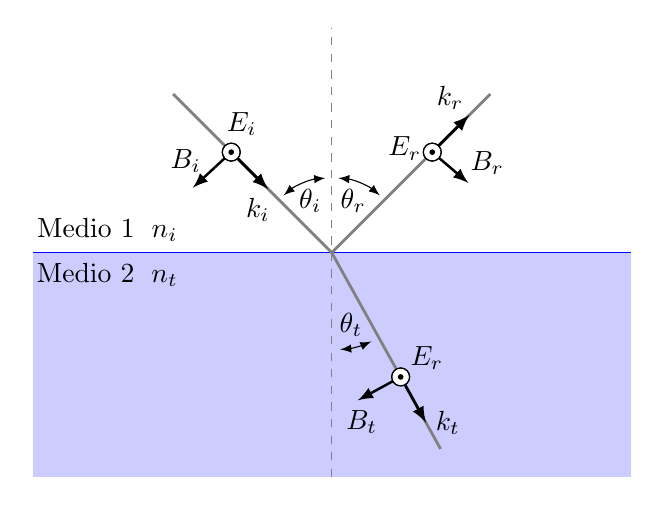
\begin{tikzpicture}[scale=.95]

%-------------------------------------------- Incidence media
\fill[blue!20] (-4,-3) rectangle (4,0);
% Interface
\draw[blue,line width=.5pt](-4,0)--(4,0); %%..5pt, interface]
% Vertical dashed line
\draw[dashed,gray,](0,-3)--(0,3);
% Media names
\node at (-3,.3) {Medio 1 $\; n_i$}; 
\node at (-3,-.3) {Medio 2 $\; n_t$};

%--------------------------------------------  Incident Wave
\draw[gray, line width=1pt](0:0cm)--(135:3cm);  % Light trajectory
\path (0,0)++(112.5:.75cm)node{$\theta_i$};       % Angle
\draw[latex-latex](95:1.cm)arc(95:130:1.cm);
 
    \draw[-latex,line width=1pt](135:1.9cm)--(135:1.2cm);    %Wave vector
    \path (0,0)++(141:0.9cm)node[left]{$\vb{k}_i$};     %Wave vector label
    
    \draw[-latex,line width=.9pt](135:1.9cm)--(155:2.05cm);  %B vector
    \path (0,0)++(148:2.3cm)node{$\vb{B}_i$}; 
    
    \path (0,0)++(125:2.1cm)node{$\vb{E}_i$};       % E vector
    
    \draw [fill= white](135:1.9cm)circle (0.12cm); % Vector perp. to surface
    \draw [black](135:1.9cm)circle (0.12cm);
    \filldraw[fill=black](135:1.9cm) circle(0.03cm); %%
    
%--------------------------------------------  Reflected Wave
\draw[gray,line width=1pt](0:0cm)--(45:3cm);  % Light trajectory
\path (0,0)++(67.5:.75cm)node{$\theta_r$};       % Angle
\draw[latex-latex](85:1.cm)arc(85:50:1.cm);
 
    \draw[-latex,line width=1pt](45:1.9cm)--(45:2.6cm);    %Wave vector
    \path (0,0)++(47.5:2.8cm)node[left]{$\vb{k}_r$};     %Wave vector label
    
    \draw[-latex,line width=.9pt](45:1.9cm)--(27:2.05cm);  %B vector
    \path (0,0)++(30:2.4cm)node{$\vb{B}_r$}; 
    
    \path (0,0)++(55:1.7cm)node{$\vb{E}_r$};       % E vector
    
    \draw [fill= white](45:1.9cm)circle (0.12cm); % Vector perp. to surface
    \draw [black](45:1.9cm)circle (0.12cm);
    \filldraw[fill=black](45:1.9cm) circle(0.03cm); %%

%--------------------------------------------  Transmitted Wave
\draw[gray,line width=1pt](0:0cm)--(-61:3cm);  % Light trajectory
\path (0,0)++(-75:1cm)node{$\theta_t$};       % Angle
\draw[latex-latex](-85:1.3cm)arc(-85:-66:1.3cm);
 
    \draw[-latex,line width=1pt](-61:1.9cm)--(-61:2.6cm);    %Wave vector
    \path (0,0)++(-61:2.6cm)node[right]{$\vb{k}_t$};     %Wave vector label

    \draw[-latex,line width=.9pt](-61:1.9cm)--(-80:2.005cm);  %B vector
    \path (0,0)++(-80:2.3cm)node{$\vb{B}_t$}; 
    
    \path (0,0)++(-48:1.9cm)node{$\vb{E}_r$};       % E vector
    
    \draw [fill= white](-61:1.9cm)circle (0.12cm); % Vector perp. to surface
    \draw [black](-61:1.9cm)circle (0.12cm);
    \filldraw[fill=black](-61:1.9cm) circle(0.03cm); %%     
 
\end{tikzpicture}
	\end{subfigure}
	\begin{subfigure}{.05\textwidth}\vspace{-4.5cm}\caption{}\label{sfig:Polp}	\end{subfigure}
	\begin{subfigure}{.43\textwidth}  \hspace*{-1cm}
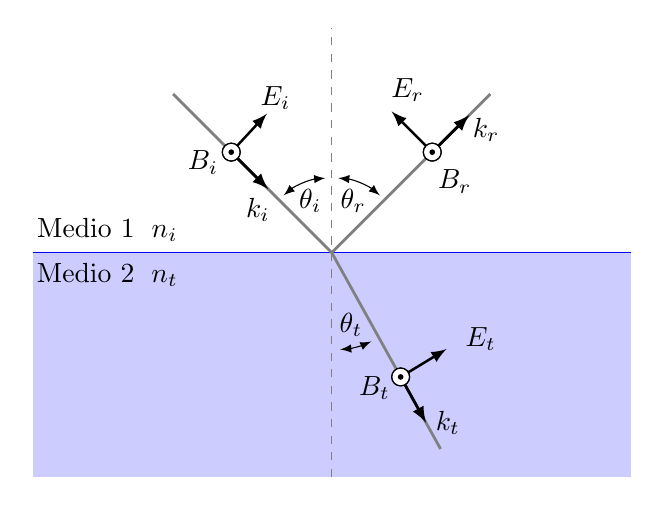
\begin{tikzpicture}[scale=.95]
%-------------------------------------------- Incidence media
\fill[blue!20] (-4,-3) rectangle (4,0);
% Interface
\draw[blue,line width=.5pt](-4,0)--(4,0); %%..5pt, interface]
% Vertical dashed line
\draw[dashed,gray,](0,-3)--(0,3);
% Media names
\node at (-3,.3) {Medio 1 $\; n_i$}; 
\node at (-3,-.3) {Medio 2 $\; n_t$};

%--------------------------------------------  Incident Wave
\draw[gray, line width=1pt](0:0cm)--(135:3cm);  % Light trajectory
\path (0,0)++(112.5:.75cm)node{$\theta_i$};       % Angle
\draw[latex-latex](95:1.cm)arc(95:130:1.cm);
 
    \draw[-latex,line width=1pt](135:1.9cm)--(135:1.2cm);    %Wave vector
    \path (0,0)++(141:0.9cm)node[left]{$\vb{k}_i$};     %Wave vector label
    
    \draw[-latex,line width=.9pt](135:1.9cm)--(115:2.05cm);  %E vector
    \path (0,0)++(110:2.2cm)node{$\vb{E}_i$}; 
%    \draw[-latex,line width=.9pt, red]((135:1.9cm)--(117:1.55cm); 

    
    \path (0,0)++(145:2.1cm)node{$\vb{B}_i$};       % B vector
    
    \draw [fill= white](135:1.9cm)circle (0.12cm);
    \draw [black](135:1.9cm)circle (0.12cm);
    \filldraw[fill=black](135:1.9cm) circle(0.03cm); %%    
    
    
%    \draw[line width=.6pt] (135:1.9cm)   % Esto esra paea hacer el vector salir de la hoja
%                         +(-135:.12cm) -- +(45:.12cm)
%                         +(-45:.12cm) -- +(135:.12cm);    
   
    
%--------------------------------------------  Reflected Wave
\draw[gray,line width=1pt](0:0cm)--(45:3cm);  % Light trajectory
\path (0,0)++(67.5:.75cm)node{$\theta_r$};       % Angle
\draw[latex-latex](85:1.cm)arc(85:50:1.cm);
 
    \draw[-latex,line width=1pt](45:1.9cm)--(45:2.6cm);    %Wave vector
    \path (0,0)++(43:2.4cm)node[right]{$\vb{k}_r$};     %Wave vector label
    
    \draw[-latex,line width=.9pt](45:1.9cm)--(67:2.05cm);  %E vector
    \path (0,0)++(65:2.4cm)node{$\vb{E}_r$};
  %  \draw[-latex,line width=.9pt, red](45:1.9cm)--(59:1.55cm); 
   % \draw[dashed,red,line width=.9pt](59:1.55cm)--(67:2.05cm);
    
    \path (0,0)++(30:1.9cm)node{$\vb{B}_r$};       % B vector
    
    \draw [fill= white](45:1.9cm)circle (0.12cm);
    \draw [black](45:1.9cm)circle (0.12cm);
    \filldraw[fill=black](45:1.9cm) circle(0.03cm); %%  


%--------------------------------------------  Transmitted Wave
\draw[gray,line width=1pt](0:0cm)--(-61:3cm);  % Light trajectory
\path (0,0)++(-75:1cm)node{$\theta_t$};       % Angle
\draw[latex-latex](-85:1.3cm)arc(-85:-66:1.3cm);
 
    \draw[-latex,line width=1pt](-61:1.9cm)--(-61:2.6cm);    %Wave vector
    \path (0,0)++(-61:2.6cm)node[right]{$\vb{k}_t$};     %Wave vector label
 
    \draw[-latex,line width=.9pt](-61:1.9cm)--(-40:2.005cm);  %E vector
%      \draw[-latex,line width=.9pt, red](-61:1.9cm)--(-45:2.3cm); 
    \path (0,0)++(-30:2.3cm)node{$\vb{E}_t$}; 
    
    \path (0,0)++(-72.5:1.9cm)node{$\vb{B}_t$};       % B vector
    
    \draw [fill= white](-61:1.9cm)circle (0.12cm);
    \draw [black](-61:1.9cm)circle (0.12cm);
    \filldraw[fill=black](-61:1.9cm) circle(0.03cm); %% 
\end{tikzpicture}
	\end{subfigure} 
	\caption{ Esquema de de una onda plana en polarización \textbf{a)} \emph{s} y \textbf{b)} \emph{p} propagándose en una dirección $\vb{k}_i$ e incidiendo con un ángulo de incidencia $\theta_i$ en una interfaz plana entre dos medio lineales, homogéneos e isótropos, donde el medio de incidencia tiene un índice de refracción $n_i$ y el de transmisión $n_t$. El haz reflejado se propaga con un ángulo $\theta_r=\theta_i$ según la ley de reflexión [Ec. \eqref{eq:LeyReflexion}] y el ángulo transmitido se propaga con un ángulo $\theta_t$ dado por la ley de Snell [Ec. \eqref{eq:LeySnell}]. En el esquema se asume que la orientación de los campos EMs incidentes  ($\vb{E}_i,\,\vb{B}_i$) es la misma para los campos EMs reflejados ($\vb{E}_r,\,\vb{B}_r$) y transmitidos ($\vb{E}_t,\,\vb{B}_t$).}	\label{fig:Polarizaciones}	
	\end{figure}	
%

Para polarización \emph{s} y medios no magnéticos ($\mu=\mu_0$),  el campo eléctrico es perpendicular al plano de incidencia y paralelo a la interfaz por lo que, mediante la Ec. \eqref{seq:Epara}, $E_i + E_r = E_t$, en donde se asume que la orientación del campo eléctrico incidente se preserva en el haz reflejado y transmitido, como se observa en la Fig. \ref{sfig:Pols}. Al emplear la continuidad de la componente paralela a la interfaz de $\vb{B}/\mu$ [Ec. \eqref{seq:Bpara}], la relación $E = (c/n) B$ y la ley de la reflexión [Ec. \eqref{eq:LeyReflexion}] y de Snell [Ec. \eqref{eq:LeySnell}] se obtienen los coeficientes de amplitud $r$ y $t$ para  polarización \emph{s}, dados por\vspace{-.5em}\index{Fresnel!coeficientes de amplitud!s}
	\begin{tcolorbox}[title = Coeficientes de amplitud para polarización \emph{s} ]
	\vspace*{-1em}	
	\eqhalf{r_s =
		\frac{n_i\cos\theta_i-\sqrt{n_t^2-n_i^2\sin ^2\theta_i}}
 			{n_i \cos\theta_i + \sqrt{ n_t^2-n_i^2\sin ^2\theta_i}}, 
 			\label{eq:rs}}
	\eqhalf{ t_s =
		\frac{2n_i\cos\theta_i}
 			{n_i\cos\theta_i + \sqrt{ n_t^2-n_i^2\sin ^2\theta_i}}.
 			\label{eq:ts}}
	\end{tcolorbox}	 \vspace*{-.5em}\noindent
Cuando el campo eléctrico es paralelo al plano de incidencia, y por tanto perpendicular a la interfaz como se observa en la Fig. \ref{sfig:Polp}, se cumple la relación $E_i\cos\theta_i-E_r\cos\theta_r = E_t \cos\theta_t$ por la Ec. \eqref{seq:Epara}. Al asumir nuevamente que la orientación de oscilación del campo eléctrico reflejado y transmitido coincide con la del campo eléctrico incidente, y al emplear las Ecs. \eqref{seq:Bpara},  \eqref{eq:LeyReflexion} y  \eqref{eq:LeySnell}, así como la relación $E = (c/n) B$, se calculan los  coeficientes de amplitud $r$ y $t$ para  polarización \emph{p}, dados por \index{Fresnel!coeficientes de amplitud!p} \vspace*{-.5em}
	\begin{tcolorbox}[title = Coeficientes de amplitud para polarización \emph{p} ]
	\vspace*{-1em}
	\eqhalf{ r_p =
				\frac{n_t^2\cos\theta_i -n_i\sqrt{n_t^2-n_i^2\sin^2\theta_i}}
 				{n_t^2\cos\theta_i +n_i\sqrt{n_t^2-n_i^2\sin^2\theta_i}}, \label{eq:rp}}
	\eqhalf{ t_p =
				\frac{ 2 n_i n_t \cos\theta_i}
 				{n_t^2\cos \theta_i+n_i\sqrt{n_t^2-n_i^2\sin^2\theta_i}}.
 				\label{eq:tp}}
	\end{tcolorbox}	

Los coeficientes  de amplitud dependen de las propiedades ópticas de los medios, descritas por los índices de refracción presentes en sus expresiones, y según el valor de los índices de refracción se presentan distintos fenómenos físicos descritos por las Ecs. \eqref{eq:rs}--\eqref{eq:tp}. Cuando la luz cruza una interfaz, entre dos medios lineales, homogéneos e isótropos, y se cumple que $n_t>n_i$, se está en una configuración de incidencia externa, mientras que en caso contrario, $n_t<n_i$, se está en  incidencia interna. En la Fig. \ref{fig:coefAmp} se grafican los coeficientes de amplitud $r$ (líneas continuas) y $t$ (líneas punteadas) como función del ángulo de incidencia $\theta_i$ para una interfaz de entre aire ($n= 1$) y un medio con un índice de refracción $n = 1.5$, en configuración de incidencia externa [Fig. \ref{sfig:coefExt}] e interna [Fig. \ref{sfig:coefInt}] para ambas polarizaciones, en donde las líneas azules corresponden a la polarización \emph{s} y las rojas a \emph{p}. Dado que los índices de refracción $n = \sqrt{\varepsilon}$ son cantidades reales, ninguno de los dos medios es absorbente. \index{Incidencia!interna}\index{Incidencia!externa}
%
\begin{figure}[h!]\centering\hspace*{-1.5em}
	\begin{subfigure}{.05\textwidth}\vspace{-4.5cm}\caption{}\label{sfig:coefExt}\end{subfigure}
	\begin{subfigure}{.43\textwidth} \hspace*{-.8cm}
	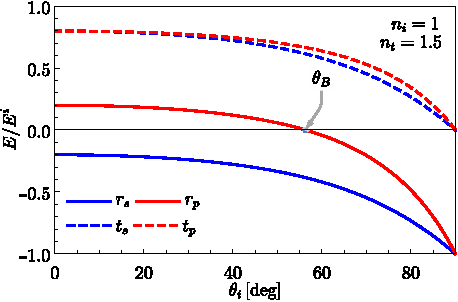
\includegraphics[scale=1]{1-Teoria/figs/1-1-ampCoefExt}
	\end{subfigure}
	\begin{subfigure}{.05\textwidth}\vspace{-4.5cm}\caption{}\label{sfig:coefInt}\end{subfigure}
	\begin{subfigure}{.43\textwidth} \hspace*{-.9cm}
	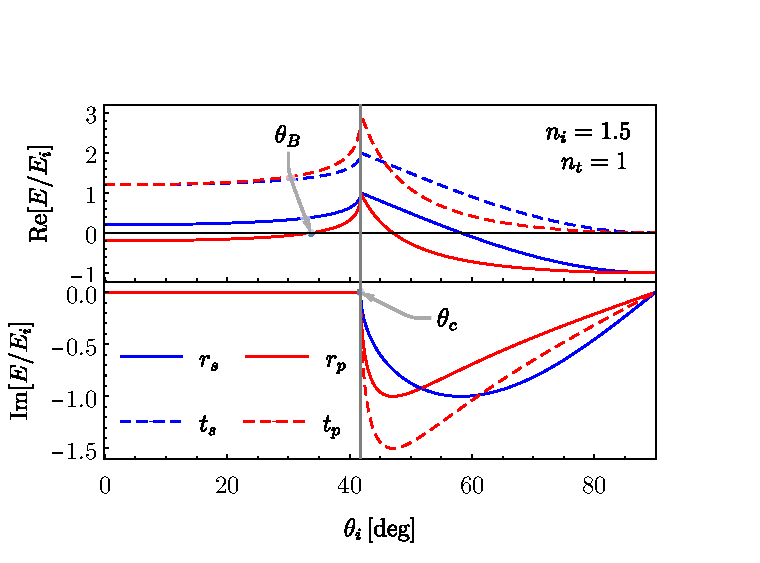
\includegraphics[scale=1]{1-Teoria/figs/1-1-ampCoefInt}
	\end{subfigure}\vspace*{-.7em}
	\caption{ Coeficientes de amplitud $r$ (líneas continuas) y $t$ (líneas punteadas), como función del ángulo de incidencia $\theta_i$, en configuración de incidencia \textbf{a)} externa e \textbf{b)} interna para una interfaz entre  aire ($n=1$) y un medio con índice de refracción $n = 1.5$. Los cálculos para polarización  \emph{s} se muestran  en azul y  para \emph{p} en rojo. }	\label{fig:coefAmp}	
	\end{figure}	
%

En la Fig. \ref{fig:coefAmp} el coeficiente de amplitud de reflexión $r_p$ [Ec. \eqref{eq:rp}] toma un valor nulo para el ángulo de incidencia  denominado ángulo de Brewster $\theta_B$, que cumple con la expresión\index{Ángulo!de Brewster} 
%
	\begin{align}
	\tan\theta_B = \frac{n_t}{n_i},
	\label{eq:Brewster}
	\end{align}
%	
tanto para incidencia externa [Fig. \ref{sfig:coefExt}], donde $\theta_B \approx 56^\circ$, como para interna [Fig. \ref{sfig:coefInt}], donde $\theta_B \approx 33^\circ$. El cambio de signo del coeficiente de reflexión $r_p$ para $\theta_i>\theta_B$ corresponde a un cambio de fase de $\pi$ radianes del campo eléctrico reflejado respecto al campo eléctrico incidente. De la Ec. \eqref{eq:Brewster} se deduce que el ángulo de Brewster de incidencia externa $\theta_B^{ext}$ es complementario al de incidencia interna $\theta_B^{int}$, es decir, $\theta_B^{ext}+\theta_B^{int} = 90^\circ$ como se observa en las gráficas de la Fig. \ref{fig:coefAmp}. Cuando se considera una configuración de incidencia interna, se cumple la relación $n_i>n_t$, por los coeficientes de amplitud  [Ecs. \eqref{eq:rs}--\eqref{eq:tp}] son cantidades complejas para un ángulos de incidencia mayores al ángulo crítico $\theta_c$ que cumple la expresión\index{Ángulo!crítico|see {Íncidencia interna}}
% 
	\begin{align}
	\sin\theta_c = \frac{n_t}{n_i}.
	\label{eq:Criticp}
	\end{align}
%
Al sustituir la Ec. \eqref{eq:Criticp} en la ley de Snell [Ec. \eqref{eq:LeySnell}] se obtiene que $\theta_t = 90^\circ$ por lo que para $\theta_i>\theta_c$ toda la luz es reflejada y no transmitida, es decir, se está en el régimen \emph{reflexión total interna}. En la Fig. \ref{sfig:coefInt} se observa que los coeficientes de amplitud son máximos en $\theta_c \approx 48^\circ$ sin embargo, para $\theta_i>\theta_c$, los coeficientes de amplitud  [Ecs. \eqref{eq:rs}--\eqref{eq:tp}] son cantidades complejas, lo que indica que los campos eléctricos reflejado y transmitido tienen un desfase, distinto de $\pi$ radianes, respecto al campo eléctrico incidente.  Para corroborar que toda la luz es reflejada en incidencia interna para $\theta_i>\theta_c$ se considera la conservación de la energía transportada por los campos EMs al cruzar la interfaz.

El análisis del comportamiento de las ondas EMs al cruzar una interfaz plana, entre dos medios lineales homogéneos e isótropos, en términos de las amplitudes de los campos eléctricos describen el comportamiento de la magnitud y los cambios de fase en los campos eléctricos  y no la cantidad de luz transmitida o reflejada. Esta información se obtiene al considerar la energía transportada por los campos EMs, por lo que se emplea el vector de Poynting [Ec. (\ref{eq:Poynting})] escrito únicamente en términos del campo eléctrico usando la relación $E = n B/c$ \index{Poynting!vector de}
	\begin{align}
	\vb{S} = n c\varepsilon_0 E_0^2 \vu{k}. \label{eq:PoyntingE}
	\end{align}
Al considerar campos eléctricos armónicos, es decir, tipo ondas planas, es necesario calcular el promedio temporal\footnote{Al considerar los campos EMs como ondas planas [Ec. \eqref{eq:OndaPlana}], el vector de Poynting es $\vb{S} = \Re(\vb{E})\times\Re(\vb{B}/\mu) = \vb{E}\times\qty(\vb{B}/\mu)^*$, en donde $*$ es el complejo conjugado y al calcular el promedio temporal $\langle\vb{S}\rangle_t = (1/\tau)\int_t^{t+\tau}\vb{S}(t')dt'$ para campos EMs tipo ondas planas, se obtiene que $\langle\vb{S}\rangle_t = (1/2) \Re[\vb{E}\times\qty(\vb{B}/\mu)^*]$.\index{Poynting!vector de!transformada de Fourier del}} de la Ec. (\ref{eq:PoyntingE}), denominado  irradiancia \cite{hecht1998optics}, dada por
	\begin{align}
	I = \langle S \rangle_t = \frac{nc\varepsilon_0}{2} E_0^2.
	\label{eq:Irr}
	\end{align}
La irradiancia $I$ corresponde a la energía promedio por unidad de tiempo, por unidad de área, transportada por los campos EMs en la dirección $\vu{k}$ \cite{griffiths2013electrodynamics}. Para calcular la energía por unidad de tiempo $P$ transportada por los campos EMs al cruzar la interfaz se multiplica la Ec. \eqref{eq:Irr} por la sección transversal del haz de luz. En la Fig. \ref{fig:hazcircular} se muestran las secciones transversales de un haz incidente que incide a un ángulo $\theta_i$ sobre la interfaz entre dos medios con índice de refracción $n_i$ y $n_t$, respectivamente. Cuando el haz se refleja, a un ángulo $\theta_r=\theta_i$, y se refracta a un ángulo $\theta_r$, la sección transversal del haz cambia. Si el área de los haces justo en la interfaz es $A$, mediante la ley de la reflexión [Ec. \eqref{eq:LeyReflexion}] y la ley de Snell [Ec. \eqref{eq:LeySnell}], la sección transversal del has incidente y el reflejado  es $A\cos\theta_i$, mientras que la del haz transmitido es $A\cos\theta_t$.

	\begin{figure}[h]\centering
\begin{tikzpicture}[scale=.7]
%\draw (3.46,1.9) circle(2pt);ESTA ES LAREFERENCIA PARA ANTES DE MOVER LAS COSAS

%---------------------------------------------------------------------------------------- SUPERFICIE
\fill[blue!20]			
(-5,-1) -- (-3,2) 
-- (3,2) -- (5,-1)
--(-5,-1);						

\draw[dashed,gray](0,-4)--(0,5);  %---------------------------------------------------- Vertical dashed line

\node at (-4,-.5) {Medio 1 $\; n_i$}; %-------------------------------------------------- media names
\node at (-4,-1.5) {Medio 2 $\; n_t$};

%---------------------------------------------------------------------------------------- SPOT INTERFAZ
\fill[lgreen, opacity= .75] (0,.5) circle (2 and .6); 
\draw[black](0,.5) circle (2 and .6)		% -------------------------------------------  Etiqueta área
			(0,.5)node[]{$A$};	
%------------------------------------------------------------- INCIDENTE
\path[shift = {(0,1.7)}] (0,0)++(112.5:1cm)node{$\theta_i$};   %---------- Angle
\draw[latex - latex,shift = {(0,2.1)}](-1,.5)arc(144.5:90:1.1cm);

\draw [-,shift = {(-2,.5)}, rotate = 55.5] (0,0) -- (0,3.2);%Cara del cilindro(Rota desde 90°)
\draw[-, shift = {(2,.5)},rotate = 55.5] (0,0) -- (0,6.3);

\draw[black, rotate = 50.75, shift = {(0,5)}](0,0) circle (1.145 and .3);% Tapa del cilidndro del del área
\node at (-5.1,3.5) { $A\cos\theta_i$};
\fill[lgreen, opacity= .5, rotate = 50.75, shift = {(0,5)}](0,0) circle (1.145 and .3);

%-------------------------------------------------------------- REFLEJADO
\path[shift = {(0,1.7)}] (0,0)++(67.5:1cm)node{$\theta_r$};   %------------- Angle
\draw[latex - latex ,shift = {(0,2.1)}](1,.5)arc(35:90:1.1cm);

\draw [-,shift = {(-2,.5)}, rotate = -55.5] (0,0) -- (0,6.3);  %- Cara del cilindro
\draw[-, shift = {(2,.5)},rotate = -55.5] (0,0) -- (0,3.2);

\draw[black, rotate = -50.75, shift = {(0,5)}](0,0) circle (1.145 and .3); %Tapa del cilidndro del del área
\node at (5.1,3.5) { $A\cos\theta_r$};
\fill[lgreen , opacity= .5, rotate = -50.75, shift = {(0,5)}](0,0) circle (1.145 and .3);

%----------------------------------------------------------------- TRANSMITIDO
\path  (0,0)++(275:4.1)node{$\theta_t$};    %------------------------- Angle
\draw[latex - latex](0,-3.5)arc(270:290:1.5cm);

\draw [-,shift = {(-2,.5)}, rotate = 33.5] (0,0) -- (0,-5);   %------------------------- Cara del cilindro
\draw[-, shift = {(2,.5)},rotate = 33.5] (0,0) -- (0,-3.1);

\draw[black, rotate = 29.2, shift = {(.5,-3.6)}](0,0) circle (1.675 and .3);		%-------- Tapa del cilidndro del del área
\node at (3.5,-3.5) {$A\cos\theta_t$};
\fill[lgreen, opacity= .5,  rotate = 29.2, shift = {(.5,-3.6)}](0,0) circle (1.675 and .3);

\end{tikzpicture}
	\caption{Sección transversal de un haz de luz incidiendo en una interfaz entre dos medio lineales, homogéneos e isótropos con índices de refracción $n_i$ y $n_t$. El haz incide sobre la interfaz a un ángulo de $\theta_i$, se refleja con un ángulo $\theta_r$ y se transmite a un ángulo $\theta_t$, calculados medinate las ley de la reflexión y de Snell, respectivamente. El área del haz sobre la interfaz es $A$, mientras que en los haces, al propagarse, es $A\cos\theta$, en donde $\theta$ es el ángulo de propagación respectivo para cada haz.} \label{fig:hazcircular}
	\end{figure}

 Al emplear la Ec. \eqref{eq:Irr} y multiplicarla por el área de alguno de los tres haces mostrados en la Fig. \ref{fig:hazcircular}, se obtiene que la energía por unidad de tiempo transportada por cada haz de luz es
	\begin{align*}
	P = I A \cos\theta = \frac{n c \varepsilon_0}{2} E_{0}^2 \cos\theta,
	\end{align*}
en donde el ángulo $\theta$ e indice de refracción $n$ toman los valores de $\theta_i$ y $n_i$ para el haz incidente y el reflejado, mientras que  toma los valores de $\theta_t$ y  $n_t$ para el haz transmitido. Cuando se normaliza la energía por unidad de tiempo transportada por el haz reflejado y por el haz transmitido, entre la del haz incidente se obtienen las expresiones de la reflectancia $R$ y la transmitancia $T$ \vspace{-.5em} \index{Fresnel!reflectancia}\index{Fresnel!transmitancia}
	\begin{tcolorbox}[title = Reflectancia y transmitancia]
	\eqhalf{ R =  r r^*, \label{eq:R}}
	\eqhalf{ T = \frac{n_t\cos\theta_i}{n_i \cos\theta_t} t t^*,\label{eq:T}}
	\end{tcolorbox}	 \vspace*{-.5em}\noindent	
en donde $r$ es el coeficiente de amplitud de reflexión y $t$ el de transmisión, dados por las Ecs. \eqref{eq:rs}--\eqref{eq:tp}, y $*$ el complejo conjugado.

En la Fig. \ref{fig:frsnel} se presentan la reflectancia (líneas continuas) y transmitancia (líneas punteadas) como función del ángulo de incidencia $\theta_i$, para la polarización \emph{s} (en azul) y \emph{p} (en rojo), de un haz de luz que incide en la interfaz entre aire ($n=1$) y un medio con índice de refracción $n=1.5$ para una configuración de incidencia externa [Fig. \ref{sfig:frsnelExt}] e incidencia interna [Fig. \ref{sfig:frsnelExt}].
%
\begin{figure}[h!]\centering\hspace*{-1.5em}
	\begin{subfigure}{.05\textwidth}\vspace{-4.5cm}\caption{}\label{sfig:frsnelExt}\end{subfigure}
	\begin{subfigure}{.43\textwidth} \hspace*{-.7cm}
	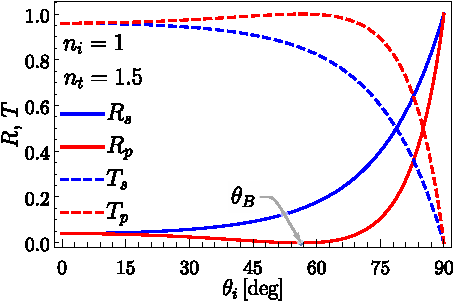
\includegraphics[scale=1]{1-Teoria/figs/1-2-FrsnelExt}
	\end{subfigure}
	\begin{subfigure}{.05\textwidth}\vspace{-4.5cm}\caption{}\label{sfig:frsenlInt}\end{subfigure}
	\begin{subfigure}{.43\textwidth} \hspace*{-.7cm}
	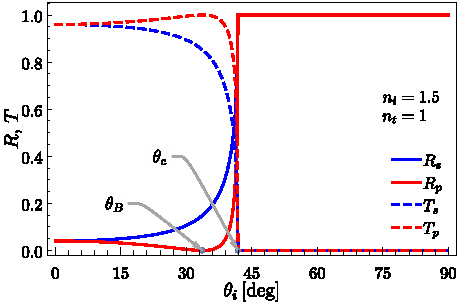
\includegraphics[scale=1]{1-Teoria/figs/1-2-FrsnelInt}
	\end{subfigure}\vspace*{-.7em}
	\caption{  Reflectrancia (líneas sólidas) y transmitancia (líneas punteadas), como función del ángulo de incidencia $\theta_i$, en configuración de incidencia \textbf{a)} externa e \textbf{b)} interna para una interfaz entre  aire ($n=1$) y un medio con índice de refracción $n = 1.5$. Los cálculos para polarización  \emph{s} se muestran  en azul y  para \emph{p} en rojo.}	\label{fig:frsnel}	
	\end{figure}	
%

El ángulo de Brewster $\theta_B$ es apreciable en las gráficas de la Fig. \ref{fig:frsnel}, en donde se observa $R_p = 0$. Asimismo es apreciable en la Fig. \ref{sfig:frsenlInt} que para ángulos de incidencia mayores al ángulo crítico, se cumple que $R_p = R_s = 1$, mientras que $T_s = T_p = 0$, es decir, que toda la luz es reflejada. En la Fig. \ref{fig:frsnel} se observa que es válida la relación 
	\begin{align*}
	R + T = 1,
	\end{align*}
sin embargo, ésta es válida únicamente para índices de refracción $n = \sqrt{\varepsilon}$ que sean cantidades reales, dado que para medios no magnéticos ($\mu_0 = \mu$), la parte imaginaria de la función dieléctrica $\Im[\varepsilon]$ se asocia con la absorción de energía por el material \cite{ibach2003solid}. Cuando la luz se propaga a través de algún medio absorbente, se cumple en general 
	\begin{align*}
	R + T + A = 1,
	\end{align*}
en donde el término $A$ es la energía absorbida por el material, relativa a la energía del haz incidente.

	
\section{Solución de Mie}

\index{Mie!solución de}
El problema de absorción y esparcimiento de luz por una partícula esférica fue resuelto por el físico alemán Gustav Mie en 1908 \cite{mie1908metallosung}.  La solución de Mie consiste en expandir una onda plana, que ilumina a una esfera de tamaño y material arbitrario, en una base de armónicos esféricos vectoriales que son una base ortogonal esférica y cuyos elementos satisfacen las ecuaciones de Maxwell \cite{bohren1998absorption}. Al considerar las condiciones de contorno que satisfacen los campos EMs sobre la superficie de la esfera,  se escriben los campos EMs dentro de la partícula y los campos esparcidos por ésta como una serie en la base de los armónicos esféricos vectoriales, cuyos coeficientes corresponden a una expanción multipolar y son conocidos como los coeficientes de Mie \cite{bohren1998absorption}. A pesar de que existen publicaciones previas a la de Mie en donde  el problema de la absorción y esparcimiento de luz es tratado de forma semejante, el trabajo de Mie destacó debido a que en él se  desarrollan relaciones recursivas que facilitan el cálculo numérico y se discute la convergencia de este resultado \cite{horvath2009historic}. El desarrollo de una solución apta para el cálculo numérico permitió que en el artículo de Mie se expusieran diez casos prácticos, los que contribuyó al impacto de su solución sobre el trabajo de otros autores \cite{horvath2009historic}. 

Para el estudio del esparcimiento por una partícula arbitraria inmersa en un medio con índice de refracción $n_m$, denominado  matriz, se considera que la partícula es iluminada por una onda plana con una longitud de onda $\lambda$, cuya dirección de propagación define la dirección $z$, es decir,
	\begin{align}
	\vb{E}^i = (E_x^i \vu{e}_x + E_y^i \vu{e}_y)e^{i(k z - \omega t)},
	\label{eq:Exyi}
	\end{align}
donde $k = 2\pi n_m /\lambda$ es el número de onda. En la Fig.  \ref{fig:PlanoEsparcimiento} se muestra  una partícula localizada en el origen iluminada por una onda plana [Ec. \eqref{eq:Exyi}] que se propaga en la dirección $z$.  De forma análoga al plano de incidencia\footnote{En el problema de un onda plana incidente a una superficie plana, el plano de incidencia se define por el vector normal a la superficie y la dirección de propagación de la onda plana.} se define el \emph{plano de esparcimiento} ( en color verde en la Fig. \ref{fig:PlanoEsparcimiento}) con el vector de dirección del esparcimiento $\vu{e}_r$ y la dirección del haz incidente $\vu{e}_z$. Con base en el plano de esparcimiento es posible definir las componentes ortogonales $\perp$ y paralelas $\parallel$ de los campos EMs, así como su polarización. 
	\begin{figure}[h!]\centering
	\tdplotsetmaincoords{60}{110}
	\pgfmathsetmacro{\rvec}{1. 3}
	\pgfmathsetmacro{\thetavec}{30}
	\pgfmathsetmacro{\varphivec}{60}
\begin{tikzpicture}[scale=3.5,tdplot_main_coords]
%draw the NP
	\draw[tdplot_screen_coords,ball color=yellow, opacity = 1] (0,0,0) circle (.05);


%set up some coordinates 
	\coordinate (O) at (0,0,0);

%determine a coordinate (P) using (r,\theta,\varphi) coordinates.   This command
%also determines (Pxy), (Pxz), and (Pyz): the xy-, xz-, and yz-projections
%of the point (P). 
%syntax: \tdplotsetcoord{Coordinate name without parentheses}{r}{\theta}{\varphi}
	\tdplotsetcoord{P}{\rvec}{\thetavec}{\varphivec}

%draw figure contents
%--------------------
%draw the main coordinate system axes
	\draw[thick,- latex] (0,0,0) -- (1. 5,0,0) node[anchor=north east]{$x$};
	\draw[thick,- latex] (0,0,0) -- (0,1. 5,0) node[anchor=north west]{$y$};
	\draw[thick,- latex] (0,0,0) -- (0,0,1. 5) node[anchor=south]{$z$};

%draw the main cartesian vector system 
	\draw[thick,- latex, blue] (0,0,0) -- (1,0,0) node[anchor= south east]{$\vu{e}_x$};
	\draw[thick,- latex, blue] (0,0,0) -- (0,1,0) node[anchor=north west]{$\vu{e}_y$};
	\draw[thick,- latex, blue] (0,0,0) -- (0,0,1) node[anchor= east]{$\vu{e}_z$};

%draw a vector from origin to point (P) 
	\draw[thick,color=green, - latex] (O) -- (P);
	\node at (1,. 5,1. 1) {\color{green} $\vb{r}$};

%draw projection on xy plane, and a connecting line
	\draw[dashed, color=green] (O) -- (Pxy);
	\draw[dashed, color=green] (P) -- (Pxy);
	\fill[green, opacity = . 3] (O) --(Pxy)-- (P)--(O);
	\node at (1,1. 5,1. 1) {\color{green}\bf Plano de esparcimiento};


%draw the angle \varphi, and label it
	%syntax: \tdplotdrawarc[coordinate frame, draw options]{center point}{r}{angle}{label options}{label}
	\tdplotdrawarc[- latex]{(O)}{0. 5}{0}{\varphivec}{anchor=south}{$\varphi$}


%set the rotated coordinate system so the x'-y' plane lies within the
	%"theta plane" of the main coordinate system
	%syntax: \tdplotsetthetaplanecoords{\varphi}
	\tdplotsetthetaplanecoords{\varphivec}

%draw theta arc and label, using rotated coordinate system
	\tdplotdrawarc[tdplot_rotated_coords, - latex]{(0,0,0)}{0. 45}{0}{\thetavec}{anchor=north}{$\theta$}

%draw some dashed arcs, demonstrating direct arc drawing
	\draw[dashed,tdplot_rotated_coords] (\rvec,0,0) arc (0:90:\rvec);
	\draw[dashed] (\rvec,0,0) arc (0:90:\rvec);

%set the rotated coordinate definition within display using a translation
%coordinate and Euler angles in the "z(\alpha)y(\beta)z(\gamma)" euler rotation convention
%syntax: \tdplotsetrotatedcoords{\alpha}{\beta}{\gamma}
	\tdplotsetrotatedcoords{\varphivec}{\thetavec}{0}

%translate the rotated coordinate system
%syntax: \tdplotsetrotatedcoordsorigin{point}
	\tdplotsetrotatedcoordsorigin{(P)}

%use the tdplot_rotated_coords style to work in the rotated, translated coordinate frame
	\draw[thick,tdplot_rotated_coords,- latex, purple] (0,0,0) -- (. 3,0,0) node[anchor=north west]{{\color{black}$\vu{e}_\theta,$}$\vu{e}_{\parallel}^s$};
	\draw[thick,tdplot_rotated_coords,- latex,black] (0,0,0) -- (0,. 3,0) node[anchor=west]{$\vu{e}_\varphi$};
	\draw[thick,tdplot_rotated_coords,- latex,purple] (0,0,0) -- (0,-. 3,0) node[anchor= north west]{$\vu{e}_{\perp}^s$};
	\draw[thick,tdplot_rotated_coords,- latex] (0,0,0) -- (0,0,. 3) node[anchor=south]{$\vu{e}_r$ };



%set the rotated coordinate definition within display using a translation
%coordinate and Euler angles in the "z(\alpha)y(\beta)z(\gamma)" euler rotation convention
%syntax: \tdplotsetrotatedcoords{\alpha}{\beta}{\gamma}
	\tdplotsetrotatedcoords{\varphivec}{0}{0}

%translate the rotated coordinate system
%syntax: \tdplotsetrotatedcoordsorigin{point}
	\tdplotsetrotatedcoordsorigin{(Pxy)}

	\draw[thick,tdplot_rotated_coords,- latex, purple] (0,0,0) -- (. 3,0,0) node[anchor= west]{$\vu{e}_{\parallel}^i$};
	\draw[thick,tdplot_rotated_coords,- latex, blue] (0,0,0) -- (0,0,. 3) node[anchor= west]{$\vu{e}_z$};	
	\draw[thick,tdplot_rotated_coords,- latex, purple] (0,0,0) -- (0,-. 3,0) node[anchor= north west]{$\vu{e}_{\perp}^i$};



% Plane Wave
	\foreach \i in {-7,...,-2}{
		\draw[thick,tdplot_screen_coords,red, - latex] (\i/10,0,0)--(\i/10,1,0);}
	\node[tdplot_screen_coords] at (-4.5/10,1.1,0){\color{red}$\vb{k}_i$};
	\node[tdplot_screen_coords] at (-4.5/10,-.1,0){\color{red}Haz incidente};
\end{tikzpicture}
%
\caption{Diagrama del plano de esparcimiento (en verde) definido por el vector $\vb{r}$, posición donde se evalúan los campos EMs, y el vector $\vu{e}_z$, cuando una onda plana propagándose en dirección $z$ (en rojo) ilumina a una partícula arbitraria.  La base canónica cartesiana para vectores se muestra en azul, mientras que la base canónica esférica se muestra en negro.  Las direcciones paralelas $\parallel$ y perpendiculares $\perp$ al plano de incidencia  para el campo eléctro incidente, denotado por el subíndice $i$ y el esparcido, denotado por el subíndice $s$ se muestran en morado.  En ambas figuras, el haz incidente se muestra en rojo.}\label{fig:PlanoEsparcimiento}
	\end{figure}	

Como se muestra en la Fig. \ref{fig:PlanoEsparcimiento}, los vectores unitarios perpendicular y paralelo al plano de esparcimiento de la onda incidente, $\vu{e}_{\perp}^i$  y $\vu{e}_{\parallel}^i$, respectivamente, están dados por \index{Plano!de esparcimiento}\index{Polarización!respecto al plano de esparcimiento|see {Plano}}\index{Polarización!respecto al plano de esparcimiento!incidente}\begin{subequations}

	\eqhalf{\vu{e}_{\perp}^i =-\, \hat{e}_\varphi  = \sin\varphi\,\vu{e}_x - \cos\varphi\,\vu{e}_y,}	
	\eqhalf{\vu{e}_{\parallel}^i = \cos\varphi\,\vu{e}_x + \sin\varphi\,\vu{e}_y,}	
	\label{eq:vecInc}\end{subequations}
	
\noindent y a su vez, la base de vectores ortonormales con la que se describirán los campos EMs esparcidos $\{\vu{e}_{\perp}^s,\vu{e}_{\parallel}^s,\vu{e}_r \}$ por la partícula son \index{Polarización!respecto al plano de esparcimiento!esparcido}

	\begin{subequations}	\eqhalf{\vu{e}_{\perp}^s= - \, \vu{e}_\varphi,}	
	\eqhalf{\vu{e}_{\parallel}^s = \vu{e}_\theta,}	
	\label{eq:vecScat}\end{subequations}
	
Al despejar $\vu{e}_x$ y $\vu{e}_y$  de las Ecs. \eqref{eq:vecInc}, y reescribirlos en la base de los vectores unitarios en la dirección perpendicular y normal al plano de esparcimiento como

	\eqhalf{\vu{e}_x = \sin\varphi\,\vu{e}_{\perp}^i + \cos\varphi\,\vu{e}_{\parallel}^i, \notag}	
	\eqhalf{\vu{e}_y = - \cos\varphi \,\vu{e}_{\perp}^i + \sin\varphi\,\vu{e}_{\parallel}^i,\notag}	

\noindent se obtiene que $\vb{E}^i$ [Ec. \eqref{eq:Exyi}] se puede escribir como
\begin{align}
\vb{E}_i = [(\cos\varphi E_{x}^i + \sin\varphi E_{y}^i)\vu{e}_{\perp}^i +
			 (\sin\varphi E_{x}^i - \cos\varphi E_{y}^i)\vu{e}_{\parallel}^i]
			 e^{ikz}
			 = E_{\perp}^i  \vu{e}_{\perp}^i + E_{\parallel}^i\vu{e}_{\parallel}^i
		\label{eq:EIncidente}
\end{align}
en donde se omite el término de la fase temporal $e^{-i\omega t}$ y la fase espacial $e^{ikz}$ se incluye en los coficientes $E_\perp^i$ y $E_\parallel^i$. Adicionalmente, al considerar para el campo eléctrico esparcido  únicamente los términos que corresponden al campo lejano, es decir, el término con componentes transversales y que decae como $r^{-1}$ y cumple con la relación $kr\ll 1$, el campo esparcido $\vb{E}^s$ puede escribirse como \cite{bohren1998absorption}\index{Campos electromagnéticos!radiativos}
	\begin{align}
	\vb{E}^s \propto \frac{e^{ikr}}{-ikr}\vb{E}_0^s 
			=  \frac{e^{ikr}}{-ikr}
			\qty( E_{\perp}^s  \vu{e}_{\perp}^s + E_{\parallel}^s \vu{e}_{\parallel}^s) \label{eq:ELejano}
	\end{align}
en donde  $\vb{E}_0^s$ es la amplitud del campo esparcido,  $ E_{\perp}^s$ y  $ E_{\parallel}^s$ sus componentes en la base de los vectores paralelo y perpendicular al plano de esparcimiento [Ec. \eqref{eq:vecScat}]. Asimismo, es posible relacionar al campo eléctrico esparcido por una partícula localizada en el centro de coordenadas$\vb{E}^s$ [Ec. \eqref{eq:ELejano}] con el  campo eléctrico incidente $\vb{E}^i$ [Ec. \eqref{eq:EIncidente}]  mediante  la diadica de esparcimiento de campo lejano  $\mathbb{F}(\vu{k}^i,\vu{k}^s)$ \cite{tsang2000scattering}
	\begin{align}
	\vb{E}^s = \frac{e^{i\vb{k}^s\cdot\vb{r}}}{r}\mathbb{F}(\vu{k}^i,\vu{k}^s)\vb{E}^i
	\label{eq:FarFieldDyadic}
	\end{align}
donde $\mathbb{F}$ depende de de la dirección de la onda plana incidente $\vu{k}^i$ y la dirección del campo eléctrico esparcido $\vu{k}^s$. Al considerar la forma asintótica del campo eléctrico esparcido [Ec. \eqref{eq:ELejano}] su relación con el campo eléctrico incidente [Ec. \eqref{eq:FarFieldDyadic}], se pueden relacionar las componentes perpendiculares del campo esparcido y el campo incidente de una onda plana en la base de los vectores perpendiculares y paralelos al plano de incidencia mediante la matriz de esparcimiento $\mathbb{S}$ \cite{bohren1998absorption}
	\begin{align}
	\mqty(E_{\parallel}^s\\E_{\perp}^s) = 
		\frac{e^{ik(r-z)}}{-ikr} \mqty(S_2&S_3\\S_4&S_1)
	\mqty(E_{\parallel}^i\\E_{\perp}^i),\label{eq:MEsparcimientoGral}
	\end{align}
en donde, de forma general, $S_j = S_j(\theta,\varphi)$, con $j=1,2,3$ y $4$, además de que las componentes de la matriz de esparcimiento en la Ec. \eqref{eq:MEsparcimientoGral} dependen de la geometría de la partícula iluminada por la onda plana.

	\subsection{Solución a la ecuación de onda con simetría esférica}


Las ecuaciones de Maxwell, al considerar una región del espacio sin cargas externas, y campos EMs armónicos en el tiempo, se reescriben como \cite{jackson1999electrodynamics} \index{Ecuaciones de Maxwell!transformada de Fourier de las}

	\begin{subequations}
	\eqhalf{\nabla\cdot \vb{E} = 0, }
	\eqhalf{\nabla\cdot \vb{H} = 0,}
	\eqhalf{\nabla \times \vb{E} = i\omega\mu \vb{H}, \label{seq:FLArm}}
	\eqhalf{\nabla\times\vb{H} = - i \omega\varepsilon \vb{E}, }	
	\label{eq:MaxwellArm}
	\end{subequations} \vspace*{-1em}
	
\noindent	
en donde $\vb{H} = \vb{B}/\mu$ es el campo H, y la función dieléctrica $\varepsilon$ y la permeabilidad magnética $\mu$ del material son funciones continuas. Al desacoplar las ecuaciones de Maxwell, se concluye que los campos EMs son soluciones a la ecuación de Helmholz \index{Ecuación!de Helmholtz}

	\begin{subequations}
	\eqhalf{\nabla^2 \vb{E}- k^2 \vb{E} = \vb{0},}
	\eqhalf{\nabla^2 \vb{H}- k^2 \vb{H} = \vb{0},}
	\label{eq:Helmholtz}
	\end{subequations} \vspace*{-1em}

\noindent	
en donde $k = n k_0$ es la magnitud del vector de onda, $n$ es el índice de refracción del material [Ec. \eqref{eq:indice}] y $k_0 = \omega / c$ es la relación de dispersión en el vacío [Ec. \eqref{eq:dispersion}].

Se propone un campo vectorial $\vb{M}$ tal que
	\begin{align}
	\vb{M} &= \nabla \times \left(\vb{r} \psi\right),
	\label{eq:MrotCPsi}
	\end{align}
donde $\psi$ es una función escalar y $\vb{r}$ el vector de posición; dado que $\vb{M}$ es el rotacional de  $\vb{r}\psi$, se cumple que $\nabla\cdot \vb{M} = \vb{0}$ y que $\vb{M}$ y $\vb{r}$ son vectores perpendiculares\footnote{Empleando la convención de la suma de Einstein y con $\epsilon_{ijk}$ el símbolo de  Levi-Civita: $M_i = [\nabla\times(\vb{c}\psi)]_i =  \epsilon_{ijk}\partial_j(r_k\psi) =\psi\epsilon_{ijk}\partial_j(r_k) -\epsilon_{ikj}r_k\partial_j\psi  =\psi[\nabla\times\vb{r}]_i - [\vb{r}\times\nabla\psi]_i = - [\vb{r}\times\nabla\psi]_i$.} La la ecuación de Helmholtz para $\vb{M}$, dado que el operador laplaciano y el rotacional conmutan\footnote{ Para un campo vectorial arbitrario $\vb{A}$ se cumple que $\nabla^2\vb{A} = \nabla(\nabla\cdot\vb{A}) - \nabla\times(\nabla\times\vb{A})$, por lo que el rotacional del laplaciano de $\vb{A}$ es $ \nabla\times( \nabla^2\vb{A})=\nabla\times[\nabla(\nabla\cdot\vb{A})  ]-  \nabla\times[\nabla\times(\nabla\times \vb{A})] = -  \nabla\times[\nabla\times(\nabla\times \vb{A})] $ pues el rotacional del gradiente de cualquier función es nulo. Además, al sustituir $\vb{A}\to \nabla\times\vb{A}$ en la expresión del laplaciano de $\vb{A}$ y  considerando que la divergencia del rotacional de cualquier función es nulo, se obtiene que$ \nabla^2(\nabla\times\vb{A})=\nabla[\nabla\cdot(\nabla\times\vb{A})  ]-  \nabla\times[\nabla\times(\nabla\times \vb{A})] = -  \nabla\times[\nabla\times(\nabla\times \vb{A})] $. Por tanto, $\nabla^2$ y $\nabla\times$ con operadores que conmutan.}, es
	\begin{align*}
	\nabla^2 \vb{M} + k^2 \nabla\vb{M} = \nabla\times \left[ \nabla^2\left(\vb{r} \psi\right)  
											+ k^2  \left(\vb{r} \psi\right) \right],
	\end{align*}
y como $\nabla^2 (\vb{r}\psi)=2\nabla\psi+\vb{r}\nabla^2\psi$\footnote{$[\nabla^2 (\vb{r}\psi)]_i = \partial^2_{jj}(r_i\psi)= \partial_j [\partial_j(r_i)\psi+r_i\partial_j\psi] =\partial_{jj}{r_i} + 2 \partial_jr_i\partial_j\psi+r_i\partial^2_{jj}\psi$, donde $\partial_j r_i = \delta_{ij}$ con $\delta_{ij}$ la delta de Kronecker, po lo que se cumple que $[\nabla^2 (\vb{r}\psi)]_i = 2\partial_i\psi+r_i\partial_{jj}\psi = 2[\nabla\psi]_i + [\vb{r}\nabla^2\psi]_i$.} y  $\nabla\times(\nabla \psi)=0$, la ecuación de Helmholtz para $\vb{M}$ puede reescribirse como
	\begin{align}
	\nabla^2 \vb{M} + k^2 \nabla\vb{M}  = \nabla\times\left[\vb{r}\left( \nabla^2\psi+k^2\psi \right) \right].
	\end{align}
Adicional a $\vb{M}$, se define el vector $\vb{N}$ dado por 
	\begin{align}
	\vb{N} = \frac{\nabla\times \vb{M}}{k}, \label{eq:NrotM/k}
	\end{align}
cuyo laplaciano es $\nabla^2 \vb{N} = \nabla^2( \nabla\times \vb{M} /k) =  \nabla\times (\nabla^2\vb{M} /k) $, y por tanto la ecuación de Helmholtz para $\vb{N}$ es
	\begin{align*}
	\nabla^2 \vb{N} + k^2 \vb{N} =  \nabla\times \left( \frac{\nabla^2 \vb{M}}{k} \right) + k \nabla\times \vb{M} 
		 = \frac{1}{k} \nabla\times \left( \nabla^2 \vb{M} + k^2  \vb{M} \right).
	\end{align*}
	
Los campos $\vb{M}$ y $\vb{N}$ cumplen con la  ecuación de Helmholtz vectorial [Ec. \eqref{eq:Helmholtz}] si, y sólo si, la función escalar $\psi$ cumple con la ecuación de Helmholtz escalar $\nabla^2 \psi + k^2 \psi = 0$. Si este es el caso, entonces, el rotacional de $\vb{N}$ está dado por
	\begin{align}
	\nabla\times \vb{N} &= \nabla\times \qty(\frac{\nabla\times \vb{M}}{k})  
						= \frac{\nabla\qty(\nabla\cdot\vb{M})-\nabla^2\vb{M}}{k}
						= - \frac{\nabla^2 \vb{M}}{k}
						= \frac{k^2 \vb{M}}{k}
						= k \vb{M}.\label{eq:rotN}
	\end{align}
	
Los campos vectoriales $\vb{M}$ y $\vb{N}$ son conocidos como los \emph{armónicos  vectoriales}, $\psi$ como su función generadora y $\vb{r}$ como el vector de guía o vector piloto. Los armónicos vectoriales $\vb{M}$ y $\vb{N}$  cumplen con tener divergencia nula y que el rotacional de uno es porporcional al otro [Ecs. \eqref{eq:NrotM/k} y \eqref{eq:rotN}], es decir, que cumplen con las ecuaciones de Maxwell[Ecs. \eqref{eq:MaxwellArm}] siempre que se cumpla que\index{Armónicos vectoriales!función generadora de los}\vspace*{-.5em}
	\begin{tcolorbox}[title = $\mathbf{\psi}$: Función generadora de los armónicos  vectoriales, ams align ]
	\nabla^2 \psi + k^2 \psi  = 0.\label{eq:AV_psi}
	\end{tcolorbox}

Cuando se considera una partícula esférica de radio $a$ e índice de refracción $n_p$, inmersa en un medio denominado matriz con índice de refracción $n_m$ (ver Fig. \ref{fig:EsferaA}), iluminada por una onda plana propagándose a lo largo del eje $z$, es conveniente emplear coordenadas esféricas $\{ r, \theta, \varphi\}$, en las que los la función generadora de los armónicos vectoriales es \index{Armónicos vectoriales!esféricos!función generadora}
	\begin{align}
	\frac{1}{r^2} \pdv{r}\qty(r^2\pdv{\psi}{r})+ 
	\frac{1}{r^2\sin\theta}\pdv{\theta}\qty(\sin\theta\pdv{\psi}{\theta})
	 + \frac{1}{r^2\sin^2\theta}\pdv[2]{\psi}{\varphi} + k^2 \psi =0, \label{eq:AEV_psi}
	\end{align}
Al resolver la Ec. \eqref{eq:AEV_psi} es posible construir un conjunto de funciones linealmente independientes que sean una base para los campos EMs incidente, esparcido y dentro de la esfera, lo que permite determinar mediante las condiciones a la frontera la forma de la matriz de esparcimiento [Ec. \eqref{eq:MEsparcimientoGral}], resolviendo el problema del esparcimiento de luz debido a la partícula.

	\begin{figure}[h!]\centering
	%set the plot display orientation
	%synatax: \tdplotsetdisplay{\theta_d}{\varphi_d}
		\tdplotsetmaincoords{60}{110}
	%define polar coordinates for some vector
	%TODO: look into using 3d spherical coordinate system
		\pgfmathsetmacro{\rvec}{1. 3}
		\pgfmathsetmacro{\thetavec}{30}
		\pgfmathsetmacro{\varphivec}{60}	
\begin{tikzpicture}[scale=4,tdplot_main_coords]

%set up some coordinates 
	\coordinate (O) at (0,0,0);

%determine a coordinate (P) using (r,\theta,\varphi) coordinates.   This command
%also determines (Pxy), (Pxz), and (Pyz): the xy-, xz-, and yz-projections
%of the point (P). 
%syntax: \tdplotsetcoord{Coordinate name without parentheses}{r}{\theta}{\varphi}
	\tdplotsetcoord{P}{\rvec}{\thetavec}{\varphivec}

%draw figure contents
%--------------------

%Draw the NP
	\draw[tdplot_screen_coords,ball color=yellow, opacity = 1] (O) circle (. 25);
	\draw[color=blue, -, thick] (0,0,0) -- (. 18,-. 18,. 18);	
	\node at (. 09,-. 09,. 15){\color{blue} $a$};
	\node at (. 25,-. 25,-. 05){$n_m$};
	\node at (. 01,-. 18,-. 1){$n_p$};		
	
%draw the main coordinate system axes
	\draw[thick,- latex] (0,0,0) -- (. 8,0,0) node[anchor=north east]{$x$};
	\draw[thick,- latex] (0,0,0) -- (0,. 8,0) node[anchor=north west]{$y$};
	\draw[thick,- latex] (0,0,0) -- (0,0,. 8) node[anchor=south]{$z$};

%draw a vector from origin to point (P) 
	\draw[thick,color=green, - latex] (O) -- (P);
	\node at (1,. 6,1. 2) {\color{green} $\vb{r}$};
	
%draw projection on xy plane, and a connecting line
	\draw[dashed, color=green] (O) -- (Pxy);
	\draw[dashed, color=green] (P) -- (Pxy);
%	\fill[green, opacity = . 3] (O) --(Pxy)-- (P)--(O);	

%draw the angle \varphi, and label it
	%syntax: \tdplotdrawarc[coordinate frame, draw options]{center point}{r}{angle}{label options}{label}
	\tdplotdrawarc[- latex]{(O)}{0. 6}{0}{\varphivec}{anchor=north}{$\varphi$}


%set the rotated coordinate system so the x'-y' plane lies within the
	%"theta plane" of the main coordinate system
	%syntax: \tdplotsetthetaplanecoords{\varphi}
	\tdplotsetthetaplanecoords{\varphivec}

%draw theta arc and label, using rotated coordinate system
	\tdplotdrawarc[tdplot_rotated_coords, - latex]{(0,0,0)}{0. 6}{0}{\thetavec}{anchor=north east}{$\theta$}

% Plane Wave
	\foreach \i in {-3,...,3}{
		\draw[thick,tdplot_screen_coords,red, - latex] (-.8+\i/10,-.3,0)--(-.8+\i/10,.7,0);}
	\node[tdplot_screen_coords] at (-8/10,+.8,0){\color{red}$\vb{k}_i$};
	\node[tdplot_screen_coords] at (-8/10,-.4,0){\color{red}Haz incidente};
\end{tikzpicture}	
		\caption{ Esfera de radio $a$ e ínidce de refracción $n_p$, inmersa en una matriz con índice $n_m$. La esfera es iluminada por una onda plana con vector de onda $\vb{k}_i$, que se propaga en la dirección $\hat{e}_z$. Se escoge como vector piloto $\vb{r}$.}\label{fig:EsferaA}
	\end{figure}	
	
Para resolver la Ec. \eqref{eq:AEV_psi} se emplea el método de separación de variables, donde se propone como solución $\psi= R(r)\Theta(\theta) \Phi(\varphi)$. Al despejar los términos que dependen únicamente de $r$ en la Ec. \eqref{eq:AEV_psi} se obtiene como resultado que una función con dependencia radial es igual a una función con dependencia angular, por lo tanto se igualan a una constante $\ell (\ell +1)$
	\begin{align}
\mathrlap{\overbrace{\phantom{\frac{1}{R} \dv{r}\qty(r^2\dv{R}{r})+  k^2 r^2 = \ell (\ell +1)}}^{\text{radial}}}
							 \frac{1}{R} \dv{r}\qty(r^2\dv{R}{r})+  k^2 r^2 = 
\mathrlap{\underbrace{\phantom{\ell (\ell +1)=
											-\frac{1}{\Theta\sin\theta}\dv{\theta}\qty(\sin\theta\dv{\Theta}{\theta})
								 			- \frac{1}{\sin^2\theta}\frac{1}{\Phi}\pdv[2]{\psi}{\varphi}. }}_{\text{angular}}}
						 	\ell (\ell +1)=
											-\frac{1}{\Theta\sin\theta}\dv{\theta}\qty(\sin\theta\dv{\Theta}{\theta})
					 						- \frac{1}{\sin^2\theta}\frac{1}{\Phi}\pdv[2]{\psi}{\varphi}.
					 		\label{eq:radAng}
	\end{align}
Si a su vez, se despejan de la parte angular de la Ec. \eqref{eq:radAng} los términos con dependencia en $\theta$ se obtiene que una función que depende únicamente de $\theta$ es igual a una que depende únicamente de $\varphi$, por lo que ambas partes se igualan a la constante $m^2$. Entonces, las funciones $R(r),\, \Theta(\theta), \mbox{ y } \Phi(\varphi)$ cumplen con las ecuaciones
\begin{align}
\frac{1}{\Phi}\dv[2]{\psi}{\varphi} &+ m^2 \Phi =0. \label{eq:Phi}\\
\frac{1}{\sin\theta}\dv{\theta}\qty(\sin\theta\dv{\Theta}{\theta}) &+ \qty[\ell(\ell+1)- \frac{m^2}{\sin^2\theta}]\Theta =0,\label{eq:Theta}\\
\dv{r}\qty(r^2\dv{R}{r}) &+ \qty[ k^2 r^2 - \ell (\ell +1)] R =0, \label{eq:R}
\end{align}
tanto $\ell$  como $m$ son constantes que se determinan ante condiciones impuestas a $\psi$. Dado que $\psi$ debe ser una función con periodicidad $2\pi$ en $\varphi$, es decir que $\psi(\varphi) = \psi(\varphi+2\pi)$, las soluciones linealmente independientes de la Ec. \eqref{eq:Phi} son \index{Armónicos vectoriales!esféricos!función generadora!solución azimutal de la}

	\begin{subequations}
	\eqhalf{\Phi_e(\varphi) = \cos(m\varphi),}
	\eqhalf{\Phi_o(\varphi) = \sin(m\varphi),}
	\label{eq:SinCos} 
	\end{subequations} \vspace{-.5em}
	
\noindent	
con $m$ un número entero no negativo y donde los subíndices $e$ y $o$ hacen referencia a que son funciones pares (\emph{even}, $e$) e impares (\emph{odd}, $o$), respectivamente. Las funciones $\sin(m\varphi)$ y $\cos(m\varphi)$ obedecen las relaciones de ortogonalidad
 	\begin{subequations}
	\begin{align}
	\int_0^{2\pi} \sin(m\varphi) &\cos(m' \varphi) \dd\varphi = 0 \qquad \forall\, m,m',\label{seq:ortSinCos}\\
	\int_0^{2\pi} \sin(m\varphi) \sin(m'\varphi)\dd\varphi &=  \int_0^{2\pi} \cos(m\varphi) \cos(m'\varphi)\dd\varphi  = \delta_{m,m'}\frac{\pi}{2},\label{seq:ortCos2}
	\end{align}\label{eq:ortSinCos}
 	\end{subequations}
en donde $\delta_{m,m'}$ es la delta de Kronecker.

Al realizar el cambio de variable $\mu = \cos\theta$ en la Ec. \eqref{eq:Theta} , ésta se reescribe como
	\begin{align*}
	\qty(1-\mu^2) \dv[2]{\Theta}{\mu} - 2 \mu \dv{\Theta}{\mu} + \qty[\ell(\ell+1)-\frac{m^2}{(1-\mu^2)}]\Theta= 0,
	\end{align*}\index{Armónicos vectoriales!esféricos!función generadora!solución polar}\index{Ecuación!asociada de Legendre}
cuyas soluciones son	las \emph{funciones asociadas de Legendre} $P_\ell^m(\cos\theta)$ de grado $\ell$ y orden $m$  \cite{arfken2001methods}, imponiendo $\ell = m, m+1,m+2,\ldots$ para  que la Ec. \eqref{eq:Theta} sea finita en $\theta = 0$ y $\theta = \pi$ ---o bien $\mu=\pm1$---. Las funciones asociadas de Legendre cumplen con la relación de ortogonalidad
	\begin{align}
	\int_{-1}^1P_\ell^m(\mu) P_{\ell'}^md\mu = \delta_{\ell,\ell'}\frac{2}{2\ell+1}\frac{(\ell+m)!}{(\ell-m)!},
	\label{eq:ortLegendre}
	\end{align}\index{Legendre!polinomios de}\index{Legendre!funciones asociadas de}
Asimismo, las funciones asociadas de Legendre se reducen a los polinomios de Legendre cuando $m=0$, ademas de que las funciones asociadas y los polinomios de Legendre se relacionan mediante la identidad 
	\begin{align}
	P_\ell^m (\mu) = (1-\mu^2)^{m/2}\dv[m]{P_\ell(\mu)}{\mu},
	\label{eq:Legendre}
	\end{align}
de donde se deduce  que $\eval{P_\ell^m(\cos\theta)}_{\theta=0,\pi}=0$ para toda $m$ distinta de cero. %Asimismo, de la Ec. \eqref{eq:FAL-PL} se obtiene que para $m=1$ se cumple que
%	\begin{align}
%	P_\ell^1(\cos\theta) = - \dv{P_\ell}{\theta} (\cos\theta ).
%	\label{eq:FALm=1}
%	\end{align}
%Además, los polinomios de Legendre cumplen con la relación de recuerrencia
%	\begin{align}
%	\dv{\theta}\qty[\sin\theta \dv{P_\ell}{\theta} ( \cos \theta ) ] = -\ell(\ell+1)\sin\theta P_\ell( \cos\theta )
%	\label{eq:PolLegeRec}
%	\end{align}

Para resolver la Ec. \eqref{eq:R} se emplea el cambio de variable $\rho = k r$ y de define la función $Z =R\sqrt{\rho}$, por lo que la Ec. \eqref{eq:R} se reescribe como
	\begin{align}
	\rho \dv{\rho}\qty(\rho\dv{Z}{\rho})+\qty[\rho^2-\qty(\ell+\frac12)^2] Z = 0,
	\label{eq:rho}
	\end{align}
cuyas soluciones son las \emph{funciones esféricas de Bessel} $j_\ell$ y $y_\ell$ o cualquier combinación lineal de ellas, por lo que de forma general las soluciones de la Ec. \eqref{eq:rho} son \cite{arfken2001methods}

	\begin{subequations}
	\eqhalf{j_\ell (\rho) = \sqrt{\frac{\pi}{2\rho}} J_{\ell+1/2}(\rho), \label{eqs:jn}}
	\eqhalf{y_\ell (\rho) = \sqrt{\frac{\pi}{2\rho}} Y_{\ell+1/2}(\rho), \label{eqs:yn}}
	\eqhalf{h_\ell^{(1)} (\rho) = j_\ell(\rho) + i y_\ell(\rho), \label{eqs:h1}}
	\eqhalf{h_\ell^{(2)} (\rho) =  j_\ell(\rho) - i y_\ell(\rho), \label{eqs:h2}}
	\label{eq:SphBessel}
	\end{subequations}

\noindent	
en donde $J_\ell$ y $Y_\ell$ son las \emph{funciones de Bessel del primer y segundo tipo} respectivamente y $h_\ell$ son las \emph{funciones esféricas de Bessel del tercer tipo}, también denominadas como \emph{funciones esféricas de Hankel}. Todas las funciones esféricas de Bessel $z_\ell$ ---donde $z_\ell$ es cualquier función de las Ecs. \eqref{eq:SphBessel}--- cumplen con las  relaciones de recurrencia
	\begin{align}
	z_{\ell-1}(\rho) + z_{\ell+1}(\rho) &=\frac{2\ell+1}{\rho} z_\ell(\rho),\\
	(2\ell + 1) \dv{z_\ell(\rho)}{\rho} &= \ell z_{\ell-1}(\rho) - (\ell+1)z_{\ell+1}(\rho),
	\end{align}
con  $j_0(\rho) = \sin\rho / \rho$ y $j_1(\rho) = \sin\rho / \rho^2- \cos\rho/\rho$, $y_0(\rho) = -\cos\rho/\rho$ y $y_1(\rho) = -\cos\rho/\rho^2-\sin\rho/\rho$.

Dado que las soluciones para la ecuación azimutal son las Ecs. \eqref{eq:SinCos}, para la polar la Ec. \eqref{eq:Legendre} y para la radial las Ecs. \eqref{eq:SphBessel}, las funciones generadoras de los armónicos esféricos vectoriales son\vspace*{-1em}

 	\begin{subequations}	\eqhalf{\psi_{em\ell} = \cos(m\varphi) P_\ell^m( \cos \theta) z_\ell(k r),}
	\eqhalf{\psi_{om\ell} = \sin(m\varphi) P_\ell^m( \cos \theta) z_\ell(k r),}
	\label{eq:psieo}	\end{subequations}

\noindent	
Al emplear las Ecs. \eqref{eq:psieo} en la Ec. \eqref{eq:MrotCPsi} se obtiene como resultado $\vb{M}_{em\ell}$ y $\vb{M}_{om\ell}$, dados por las expresiones \vspace{-.5em}
	\begin{subequations}
	\begin{tcolorbox}[title = Armónicos esféricos vectoriales $\vb{M}_{em\ell}$ y $\vb{M}_{om\ell}$, ams align ]
	\vb{M}_{em\ell} = &-m\sin(m\varphi)z_\ell(kr) \frac{P_\ell^m(\cos\theta)}{\sin\theta}\,\vu{e}_\theta
					-\cos(m\theta)z_\ell(kr) \dv{P_\ell^m(\cos\theta)}{\theta}(\cos\theta)\,\vu{e}_\varphi,\label{seq:Meml} \\
	\vb{M}_{om\ell} = & m\cos(m\varphi)z_\ell(kr) \frac{P_\ell^m(\cos\theta)}{\sin\theta}\,\vu{e}_\theta
					-\sin(m\theta)z_\ell(kr) \dv{P_\ell^m(\cos\theta)}{\theta}(\cos\theta)\,\vu{e}_\varphi.	\label{seq:Moml}				
	\end{tcolorbox} \noindent
%
Para el cálculo $\vb{N}_{em\ell}$ y $\vb{N}_{om\ell}$ se sustituyen las Ecs. \eqref{seq:Meml} y \eqref{seq:Moml} en la Ec. \eqref{eq:NrotM/k}. Para simplificar las expresiones de las componentes radiales de  $\vb{N}_{em\ell}$ y $\vb{N}_{om\ell}$, se agrupan los términos que dependen de $\varphi$ y $kr$ y, dado que las funciones asociadas de Legendre cumplen con la relación 
\begin{align*}
-\ell(\ell+1) P_\ell^m (\cos\theta)= \frac{1}{\sin\theta}\dv{\theta}\qty(\sin\theta\dv{P_\ell^m(\cos\theta)}{\theta}) - \frac{m^2}{\sin^2\theta}P_\ell^m(\cos\theta),
\end{align*}
que es una consecuencia de la Ec. \eqref{eq:Theta}, las expresiones de $\vb{N}_{em\ell}$ y $\vb{N}_{om\ell}$ son \vspace*{-.5em}
%
	\begin{tcolorbox}[title = Armónicos esféricos vectoriales $\vb{N}_{em\ell}$ y $\vb{N}_{om\ell}$, ams align, breakable ]
	\vb{N}_{em\ell} =&\cos(m\varphi) \frac{z_\ell(kr)}{kr} \ell(\ell+1)P_\ell^m(\cos\theta)\,\vu{e}_r\notag\\
	&+ \cos(m\varphi)  \frac{1}{kr} \dv{(kr)}\qty\Big[kr\, z_\ell(kr)] \dv{P_\ell^m(\cos\theta)}{\theta}(\cos\theta)\,\vu{e}_\theta
	 \label{seq:Neml} \\
		&- m \sin(m\varphi) \frac{1}{kr} \dv{(kr)}\qty\Big[kr\, z_\ell(kr)] \frac{P_\ell^m(\cos\theta)}{\sin\theta}
		 \,\vu{e}_\varphi, \notag\\			
	\vb{N}_{om\ell} =&\sin(m\varphi)\frac{z_\ell(kr)}{kr} \ell(\ell+1)P_\ell^m(\cos\theta)\,\vu{e}_r \notag\\
	&+ \sin(m\varphi)  \frac{1}{kr} \dv{(kr)}\qty\Big[kr\, z_\ell(kr)] \dv{P_\ell^m(\cos\theta)}{\theta}(\cos\theta) \,\vu{e}_\theta
	 \label{seq:Noml} \\
		&+ m \cos(m\varphi) \frac{1}{kr} \dv{(kr)}\qty\Big[kr\, z_\ell(kr)] \frac{P_\ell^m(\cos\theta)}{\sin\theta}
		\, \vu{e}_\varphi. \notag							
	\end{tcolorbox}\label{eq:AEV}
	\end{subequations}

Los armónicos esféricos vectoriales son solución a la ecuación de Helmholtz, por lo que cualquier solución de los campos EM puede escribirse como una serie infinta en términos de las Ecs. \eqref{eq:AEV}. Para resolver el problema de los campos EMs esparcidos por una partícula esférica, estos es, determinar las componentes de la matriz de esparcimiento $\mathbb{S}$ de la Ec. \eqref{eq:MEsparcimientoGral}, se expande una onda plana $\vb{E}^i$ en la base de los armónicos esféricos vectoriales. Para esto, se emplean sus  condiciones de ortogonalidad, calculadas a partir de la relaciones de ortogonalidad de las Ecs. \eqref{eq:SinCos} y \eqref{eq:ortLegendre}, dando como resultado que los armónicos esféricos vectoriales son ortogonales cuando tienen paridad distinta y cuando se realiza el producto interior entre $\vb{M}$ y $\vb{N}$, es decir \vspace{-.5em}
%
	\begin{tcolorbox}[ ams align ]
		\langle\vb{M}_{em\ell}, \vb{M}_{om'\ell'} \rangle_{\theta,\varphi} =
		\langle\vb{N}_{em\ell}, \vb{N}_{om'\ell'} \rangle_{\theta,\varphi} = 0
		&\qquad \forall\,  m,m',\ell, \ell',\\
		\langle\vb{M}_{om\ell}, \vb{N}_{em'\ell'} \rangle_{\theta,\varphi} = 
		\langle\vb{M}_{om\ell}, \vb{N}_{om'\ell'} \rangle_{\theta,\varphi} = 	
		\langle\vb{M}_{em\ell}, \vb{N}_{em'\ell'} \rangle_{\theta,\varphi} = 0
		&\qquad \forall\,  m,m',\ell, \ell',	\\
		\langle\vb{M}_{em\ell},  \vb{N}_{om\ell'} \rangle_{\theta,\varphi} =
		\langle\vb{M}_{om\ell},  \vb{N}_{em\ell'} \rangle_{\theta,\varphi} = 0	
		&\qquad \forall\, \ell, \ell'\, m,
	\end{tcolorbox}\vspace{-.5em}\noindent
en donde se definió el producto interior $\langle \vb{A},\vb{B} \rangle_{\theta,\varphi}$ como 
	\begin{align*}
	\langle \vb{A},\vb{B} \rangle_{\theta,\varphi} 
	\equiv 
	\int_0^{2\pi}\int_0^\pi \vb{A}\cdot\vb{B} \sin\theta \dd\theta \dd\varphi.
	\end{align*}
De igual manera, cuando se realiza el producto interior con elementos de los armónicos esféricos vectoriales de la misma paridad, y considerando las combinaciones de  $\langle \vb{M},\vb{M}\rangle$ y $\langle \vb{N},\vb{N}\rangle$  se obtienen las relaciones \vspace{-.5em}
	\begin{tcolorbox}[ ams align ]
	\!\!	\langle\vb{M}_{em\ell},  \vb{M}_{em\ell'} \rangle_{\theta,\varphi} = 
		&\langle\vb{M}_{om\ell},  \vb{M}_{om\ell'} \rangle_{\theta,\varphi} 
			=\delta_{\ell,\ell'}\pi z_\ell (\rho)^2
			\frac{\ell(\ell+1)}{2\ell+1}\frac{(\ell+m)!}{(\ell-m)!}
		\quad \forall\, \ell, \ell',\, m, \label{eq:MM} \\
	\!\!	\langle\vb{N}_{em\ell},  \vb{N}_{em\ell'} \rangle_{\theta,\varphi} = 
		&\langle\vb{N}_{om\ell},  \vb{N}_{om\ell'} \rangle_{\theta,\varphi}
		 \label{eq:NN}\\
			=&\delta_{\ell,\ell'}\pi\frac{\ell(\ell+1)}{2\ell+1}
			\frac{(\ell+m)!}{(\ell-m)!}
			\left\{ \qty[\frac{z_\ell(\rho)}{\rho}]^2 \ell(\ell+1)+
			 \qty[\frac{1}{\rho}\dv{[\rho z_\ell (\rho)]}{\rho}]^2  \right\}
		\quad \forall\, \ell, \ell',\, m.	\notag
	\end{tcolorbox}

%------------------------------

Al considerar una onda plana con longitud de onda $\lambda$, polarizada en la dirección $x$, y caracterizada por el campo eléctrico $\vb{E}^i$ propagándose en la dirección $z$ en una matriz con índice de refracción $n_m = \sqrt{\varepsilon_m\mu_m / \varepsilon_0\mu_0}$ (ver Fig. \ref{fig:EsferaA}), en la base de los vectores ortonormales polares canónicos, así como en la base de los armónicos esféricos vectoriales [Ecs. \eqref{eq:AEV}] es
	\begin{align*}
\vb{E}^i = & E_0 e^{ik_mr\cos\theta} \qty(\sin\theta\cos\varphi \vu{e}_r + 
								\cos\theta\cos\varphi\vu{e}_\theta-\sin\varphi\vu{e}_\varphi)\notag\\
	 =& \sum_{m=0}^\infty\sum_{\ell=m}^\infty \qty[ B_{em\ell}\vb{M}_{em\ell} 
	 	+ B_{om\ell}\vb{M}_{om\ell} +A_{em\ell}\vb{N}_{em\ell} + A_{om\ell}\vb{N}_{om\ell}].,
	\end{align*}
donde se omite la dependencia temporal $e^{-i\omega t}$, $E_0$ es la magnitud del campo eléctrico, $k_m=2\pi n_m/\lambda$ es el número de onda,  y  $B_{em\ell},\, B_{om\ell},\, A_{em\ell}$ y $ A_{om\ell}$ son los coeficientes en la expansión de armónicos esféricos vectoriales de la onda plana, que se determinan a partir de las Ecs. \eqref{eq:NN} y \eqref{eq:MM}. Dado que en la componente radial de la onda plana en la base canónica es proporcional a $\cos\varphi$, se sigue que $m=1$ al comparar con las expresiones de $\vb{N}_{em\ell}$ [Ec. \eqref{seq:Neml}] y $\vb{N}_{om\ell}$ [Ec. \eqref{seq:Noml}] ---únicos elementos con componente radial---, y además que $A_{om\ell}=0$ pues $\vb{N}_{om\ell}$ es proporcional a $\sin\varphi$ en la componente radial. Asimismo, por la dependencia con $\sin\varphi$ en la componente  $\vu{e}_\varphi$, $B_{em\ell}=0$ pues $\vb{M}_{em\ell}$ es proporcional a $\cos\varphi$ en dicha entrada. Puesto que la onda plana es finita en todo el espacio, se escoge $z_\ell = j_\ell$, denotado en los armónicos esféricos vectoriales con el superíndice $(1)$. Entonces, la onda plana en la base de los armónicos esféricos vectoriales se escribe como 
	\begin{align*}
	\vb{E}^i = \sum_{\ell=1}^\infty \qty[B_{o1\ell}\vb{M}_{o1\ell}^{(1)} + A_{e1\ell}\vb{N}_{e1\ell}^{(1)}],
	\end{align*}
con $B_{o1\ell} = \langle \vb{E}^i, \vb{M}_{o1\ell}^{(1)}  \rangle_{\theta,\varphi} / \langle \vb{M}_{o1\ell}^{(1)} ,\vb{M}_{o1\ell}^{(1)} \rangle_{\theta,\varphi}$ y $ A_{e1\ell} = \langle \vb{E}^i, \vb{N}_{e1\ell}^{(1)} \rangle_{\theta,\varphi} / \langle \vb{N}_{e1\ell}^{(1)},\vb{N}_{e1\ell}^{(1)} \rangle_{\theta,\varphi}$. Al emplear las Ecs. \eqref{eq:MM} y \eqref{eq:NN} con $m=1$, y las condiciones de ortogonalidad de los armónicos esféricos vectoriales, se calcula la expresión de la onda plana en una base esférica, dada por
	\begin{subequations}
	\begin{align}
	\vb{E}^i = E_0 \sum_{\ell =1}^\infty i^\ell \frac{2\ell+1}{\ell(\ell+1)}\qty(\vb{M}_{o1\ell}^{(1)}-i\vb{N}_{e1\ell}^{(1)}).
	\label{eqs:EiAEV}
	\end{align}
El campo magnético incidente se calcula empleando la Ley de Farady-Lenz [Ec. \eqref{seq:FLArm}], cuyo resultado es
	\begin{align}
	\vb{H}^i =\frac{-k_m}{\omega\mu_m} \sum_{\ell =1}^\infty  E_\ell\qty(\vb{M}_{e1\ell}^{(1)}+i\vb{N}_{o1\ell}^{(1)}),
	\label{eqs:HiAEV}
	\end{align}\label{eq:EHiAEV}
	\end{subequations}
con $E_\ell = E_0 i^\ell (2\ell+1)/[\ell(\ell+1)]$.

Para calcular los campos EMs esparcidos ($\vb{E}^s,\,\vb{H}^s$) y los campos EMs dentro de la partícula esférica ($\vb{E}^p,\,\vb{H}^p$), se emplean las condiciones a la frontera de los campos EMs en una interfaz arbitraria [Ecs. \eqref{eqs:CFrontera}], en donde la componente paralela a la interfaz es continua. Es decir
	\begin{align}
	\qty(\vb{E}^i+\vb{E}^s -\vb{E}^p)\times\vu{e}_r =
	\qty(\vb{H}^i+\vb{H}^s -\vb{H}^p)\times\vu{e}_r = \vb{0}.
	\label{eq:CFEsfera}
	\end{align}
De las Ecs. \eqref{eq:EHiAEV} y de las condiciones a la frontera [Ec. \eqref{eq:CFEsfera}], se deduce que en la expansión de los campos EMs esparcidos, y los internos, los coeficientes para $m\neq 1$ son nulos. Los campos EMs dentro de la partícula ($\vb{E}^p,\,\vb{H}^p$) son finitos en la esfera, por lo que se emplea como solución a la ecuación de onda las funciones $j_\ell(k_p r)$, con $k_p = 2\pi n_p /\lambda$ el número de onda dentro de la esfera. Las expresiones para los campos EMs son
	
	\begin{subequations}
	\eqhalf{\vb{E}^p = \sum_{\ell =1}^\infty E_\ell \qty(c_\ell \vb{M}_{o1\ell}^{(1)}-i d_\ell\vb{N}_{e1\ell}^{(1)}),	\label{eqs:EpAEV}}
	\eqhalf{\vb{H}^p = \frac{-k_p}{\omega\mu_p} \sum_{\ell =1}^\infty E_\ell\qty(d_\ell\vb{M}_{e1\ell}^{(1)}+i c_\ell\vb{N}_{o1\ell}^{(1)}),\label{eqs:HpAEV}}
	\label{eq:EHpAEV}		
	\end{subequations}

Para los campos esparcidos ($\vb{E}^s,\,\vb{H}^s$) las funciones $j_\ell$ y $y_\ell$ no tienen puntos indeterminados, por lo que se emplearan las funciones esféricas de Hankel $h_\ell^{(1)}$ y $h_\ell^{(2)}$, que en su límite asintótico ($\ell^2\ll kr$), son \cite{bohren1998absorption}

	\eqhalf{h_\ell^{(1)}(k_m r) \approx -i^\ell \frac{e^{ik_m r}}{ik_m r},\notag}
	\eqhalf{h_\ell^{(2)}(k_m r) \approx -i^\ell \frac{e^{-ik_m r}}{ik_m r},\notag}	

\vspace*{-1em}\noindent
por lo que $h_\ell^{(1)}$ corresponde a una onda esférica saliente, y $h_\ell^{(2)}$ una entrante. Dado que el campo esparcido es una onda saliente, se emplea $h_\ell^{(1)}$ como solución radial a la función generadora de los armónicos esféricos vectoriales. Entonces, los campos EMs esparcidos $(\vb{E}^s,\vb{H}^s)$ son 
	\begin{subequations}
	\eqhalf{\vb{E}^s = \sum_{\ell =1}^\infty E_\ell \qty(i a_\ell \vb{N}_{e1\ell}^{(3)}- b_\ell\vb{M}_{o1\ell}^{(3)}),
		\label{eqs:EsAEV}}
	\eqhalf{\vb{H}^s = \frac{k}{\omega\mu} \sum_{\ell =1}^\infty E_\ell\qty(ib_\ell\vb{N}_{o1\ell}^{(3)}+a_\ell\vb{M}_{e1\ell}^{(3)}),
		\label{eqs:HsAEV}}	
	\label{eq:EHsAEV}		
	\end{subequations}
		
\noindent
en donde se denota mediante el superíndice $(3)$ que se emplea $h_\ell^{(1)}$ para la solución radial. Dado que para los campos EMs de la onda plana incidente, para de los campos EMs esparcidos y los campos EMs dentroe de la partícula se cumple que $m= 1$, se definen las funciones   $\pi_\ell$ y $\tau_\ell$ como  

	\begin{subequations}
	\eqhalf{\pi_\ell(\cos\theta)= \frac{P_\ell^1(\cos\theta)}{\sin\theta},
		\label{eqs:pi}}
	\eqhalf{\tau_\ell(\cos\theta) = \dv{P_\ell^1(\cos\theta)}{\theta},
		\label{eqs:tau}}	
	\label{eq:pitau}		
	\end{subequations}

\noindent
para expresar la dependencia angular polar en los armónicos esféricos vectoriales [Ecs. \eqref{eq:AEV}]. Las relaciones de recurrencia de las funciones asociadas de Legendre \cite{arfken2001methods} permiten expresar a  $\pi_\ell$ y $\tau_\ell$ como  \cite{bohren1998absorption}

	\eqhalf{\pi_\ell(\mu) = \frac{2\ell-1}{\ell-1} \mu \pi_{\ell-1}(\mu) - \frac{\ell}{\ell-1}\pi_{\ell-2}(\mu),
		\notag}
	\eqhalf{\tau_\ell(\mu) = \ell \mu\pi_\ell(\mu) - (\ell+1)\pi_{\ell-1}(\mu),
		\notag}	

\noindent
en donde se empleó el cambio de variable $\mu = \cos\theta$ y se define   $\pi_0 =0 $ y $\pi_1 = 1$.  Las funciones $\pi_\ell$ y $\tau_\ell$ son funciones pares e impares, respectivamente, y a pesar de no ser orotogonales, sí lo son la suma aritmética de ellas, es decir
	\begin{align}
	\int_{-1}^{1}[\tau_\ell(\mu)\pm\pi_\ell(\mu)]
	[\tau_{\ell'}(\mu)\pm\pi_{\ell'}(\mu)] = 0, \qquad \ell\neq \ell'. 
	\label{eq:ortTauPi}
	\end{align}

Para determinar los coeficientes $a_\ell,b_\ell,c_\ell$ y $d_\ell$ de las Ecs. \eqref{eq:EHpAEV} y \eqref{eq:EHsAEV} se emplean las condiciones a la frontera [Ec. \eqref{eq:CFEsfera}], por lo que se deben de satisfaces las ecuaciones

	\eqhalf{E_\theta^i + E_\theta^s = E_\theta^p,\notag}
	\eqhalf{E_\varphi^i + E_\varphi^s = E_\varphi^p,\notag}
	\eqhalf{H_\theta^i + H_\theta^s = H_\theta^p,\notag}
	\eqhalf{H_\varphi^i + H_\varphi^s = H_\varphi^p,\notag}\vspace*{-1em}

\noindent
en $r =a$, que es la superficie de la partícula esférica. Al emplear la ortogonalidad de las funciones $\sin\varphi$ y $\cos\varphi$ [Ec. \eqref{eq:ortTauPi}], rescribir los armónicos esféricos vectoriales [Ecs. \eqref{eq:AEV}] en términos de $\pi_\ell$ y $\tau_\ell$ y emplear la ortogonalidad de $\tau_\ell\pm\pi_\ell$ [Ec. \eqref{eq:ortTauPi}], junto con las expresiones de los campos EMs de la onda plana incidente [Ecs. \eqref{eq:EHiAEV}], de los campos EMs dentro de la partícula [Ecs. \eqref{eq:EHpAEV}] y los campos EMs esparcidos [Ecs. \eqref{eq:EHsAEV}] se obtienen el sistema de ecuaciones
	\begin{align*}
	j_\ell(Nx)c_\ell + h_\ell^{(1)}(x)b_\ell &= j_\ell(x),\\
	\mu_m\qty[Nj_\ell(Nx)]'c_\ell + \mu_p [xh_\ell^{(1)}(x)]'b_\ell &= \mu_p [xj_\ell(x)]',\\
	\mu_m N j_\ell(Nx)d_\ell +\mu_p h_\ell^{(1)}(x)a_\ell &=\mu_p j_\ell(x),\\
	\qty[Nj_\ell(Nx)]'d_\ell + N [xh_\ell^{(1)}(x)]'a_\ell &= N [xj_\ell(x)]',
	\end{align*}
en donde $'$ denota la derivada respecto al argumento de las funciones de Bessel, $x = k_m a = 2 \pi n_m a /\lambda$ es el parámetro de tamaño y $N = n_p / n_m$ es el índice de refracción relativo entre la partícula y la matriz. Al determinar los coeficientes $a_\ell$ y $b_\ell$, se obtiene una expresión analítica para los campos EMs esparcidos, por lo que es posible determinar las componentes de la matriz de esparcimiento $\mathbb{S}$ en la Ec. \eqref{eq:MEsparcimientoGral}. La solución para los coeficientes $a_\ell$ y $b_\ell$, los coeficientes de los campo EMs esparcidos\footnote{Las expresiones de los coeficientes para los campos EMs dentro de la partícula esférica [Ec. \eqref{eq:EHpAEV}] son
	\begin{align*}
	c_\ell = \frac{\mu_p j_\ell(x)[xh_\ell^{(1)}(x)]' - \mu_p h_\ell^{(1)}(x) [xj_\ell(x)]'}
				{\mu_pj_\ell(Nx) [xh_\ell^{(1)}(x)]'-\mu_m h_\ell^{(1)}(x) [N x j_\ell(Nx)]' },
	\qquad	
	d_\ell = \frac{\mu_p N j_\ell(x)[xh_\ell^{(1)}(x)]' - \mu_p N h_\ell^{(1)}(x) [xj_\ell(x)]'}
				{\mu_m N^2 j_\ell(Nx) [xh_\ell^{(1)}(x)]'-\mu_p h_\ell^{(1)}(x) [N x j_\ell(Nx)]' }	,
	\end{align*}}, son
	\begin{subequations}\begin{align}
	a_\ell &= \frac{\mu_m N^2 j_\ell(Nx)[xj_\ell(x)]' - \mu_p j_\ell(x) [Nxj_\ell(x)]'}
				{\mu_mN^2j_\ell(Nx) [xh_\ell^{(1)}(x)]'-\mu_p h_\ell^{(1)}(x) [N x j_\ell(Nx)]' },
	\label{eq:a_ellFULL}\\
	b_\ell &= \frac{\mu_p N j_\ell(Nx)[xj_\ell(x)]' - \mu_m j_\ell(x) [Nxj_\ell(x)]'}
				{\mu_p j_\ell(Nx) [xh_\ell^{(1)}(x)]'-\mu_m h_\ell^{(1)}(x) [N x j_\ell(Nx)]' },
	\label{eq:b_ellFULL}			
	\end{align}\label{eq:MieCoefScattFULL}\end{subequations}
sin embargo, para el caso en el que la partícula esférica no es magnéntica, es decir $n_p = \sqrt{\varepsilon_p/\varepsilon_0}$, las Ecs. \eqref{eq:MieCoefScattFULL} se reescriben como\begin{subequations}\vspace*{-.5em}
	\begin{tcolorbox}[title = Coeficientes de Mie, ams align, breakable ]
	a_\ell &= \frac{N\psi_\ell(Nx)\psi_\ell'(x)-\psi_\ell(x)\psi_\ell' (Nx)}
				{N\psi_\ell(Nx)\xi_\ell'(x)-\xi_\ell(x)\psi_\ell'(Nx)},
				\label{eqs:a_ell}\\
	b_\ell &= \frac{\psi_\ell(Nx)\psi_\ell'(x)-N\psi_\ell(x)\psi_\ell' (Nx)}
			{\psi_\ell(Nx)\xi_\ell'(x)-N\xi_\ell(x)\psi_\ell'(Nx)},
			 \label{eqs:b_ell}	 
	\end{tcolorbox}\label{eq:MieCoef}	\end{subequations}\vspace*{-.5em}\noindent
en donde $\psi_\ell(\rho) = \rho j_\ell(\rho)$ y $\xi_\ell(\rho) = \rho h_\ell^{(1)}(\rho)$  son las funciones de Riccati-Bessel \cite{bohren1998absorption,arfken2001methods} y los términos $\psi'_\ell$ y $\xi'_\ell$ denotan las derivadas de las funciones respecto a su argumento. Los armónicos esféricos vectoriales representan una expansión multipolar del campo eléctrico esparcido por una partícula esférica y los coeficientes de Mie [Ec.  \eqref{eq:MieCoef}] modulan la contribución al campo total esparcido de cada término:  $a_\ell$, los multipolos eléctricos; $b_\ell$, los magnéticos \cite{kreibig1995clusters}. En la Fig. \ref{fig:Multipolos} se muestran la contribuciones multipolares del campo eléctrico esparcido\footnote{En el artículo original de Mie (ref. \cite{mie1908metallosung}) se les denomina a la contribuciones multipolares como ondas parciales.} $\vb{E}^s$ [Ec. \eqref{eqs:EsAEV}], considerando únicamente las componentes transversal a una  superficie esférica y concéntrica a la partícula esparcidora. 
%	\begin{figure}[h]\centering
%		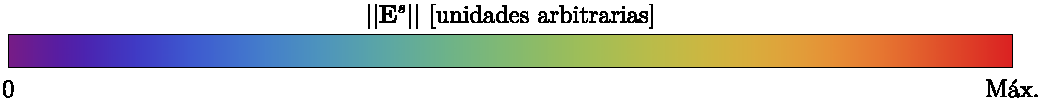
\includegraphics[scale=.85]{1-Teoria/figs/EsNorm.pdf}\\
%		\hspace{-4em}
%		\begin{subfigure}{.05\linewidth}\vspace{-3.25cm}\label{figs:ElectricMultipoles} \caption{ } \end{subfigure}
%		\hspace{-3em}
%		\begin{subfigure}{.9\linewidth}
%		\animategraphics[loop, autoplay,scale=.25]{10}{1-Teoria/figs/Ne11/Ne11_crop-}{0}{62}%
%		\animategraphics[loop, autoplay,scale=.25]{10}{1-Teoria/figs/Ne12/Ne12_crop-}{0}{62}%
%		\animategraphics[loop, autoplay,scale=.25]{10}{1-Teoria/figs/Ne13/Ne13_crop-}{0}{62}%
%		\animategraphics[loop, autoplay,scale=.25]{10}{1-Teoria/figs/Ne14/Ne14_crop-}{0}{62}
%		\end{subfigure}\\
%		\hspace{-4em}	
%		\begin{subfigure}{.05\linewidth}\vspace{-3.25cm}\label{figs:MagneticMultipoles} \caption{ } \end{subfigure}
%		\hspace{-3em}
%		\begin{subfigure}{.9\linewidth}			
%		\animategraphics[loop, autoplay,scale=.25]{10}{1-Teoria/figs/Mo11/Mo11_crop-}{0}{62}%
%		\animategraphics[loop, autoplay,scale=.25]{10}{1-Teoria/figs/Mo12/Mo12_crop-}{0}{62}%
%		\animategraphics[loop, autoplay,scale=.25]{10}{1-Teoria/figs/Mo13/Mo13_crop-}{0}{62}%
%		\animategraphics[loop, autoplay,scale=.25]{10}{1-Teoria/figs/Mo14/Mo14_crop-}{0}{62}%
%		\end{subfigure}
%		\caption{Contribuciones multipolares \textbf{a)} eléctricas $a_\ell$ y \textbf{b)} magnéticas $b_\ell$ de orden $\ell = 1,2,3$ y $4$ del campo esparcido $\vb{E}^s$ por una partícula esférica, evaluadas en una superficie matemática esférica y concéntrica a la partícula que radía los campos EMs, en donde el plano de la página corresponde al plano de oscilación del campo eléctrico incidente $\vb{E}^i$. En las gráficas presentadas, el color rojo corresponde a los valores máximos del campo eléctrico, mientras que los azules son los puntos menos intensos, donde se presentan los nodos en la superficie esférica.}
%		\label{fig:Multipolos}
%	\end{figure}
	\begin{figure}[h!]\centering
		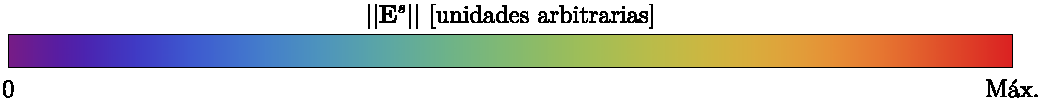
\includegraphics[scale=.85]{1-Teoria/figs/EsNorm.pdf}\\
		\hspace{-4em}
		\begin{subfigure}{.05\linewidth}\vspace{-3.25cm}\label{figs:ElectricMultipoles} \caption{ } \end{subfigure}
		\hspace{-3em}
		\begin{subfigure}{.9\linewidth}
			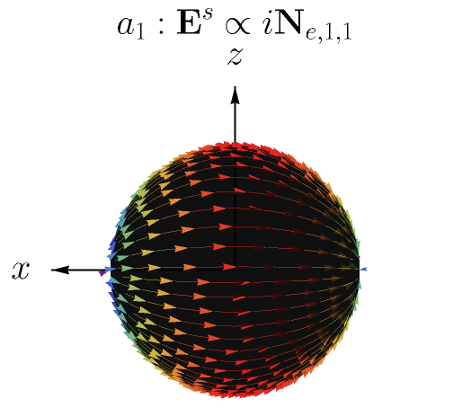
\includegraphics[scale=.25]{1-Teoria/figs/Ne11_static_crop.png}%
			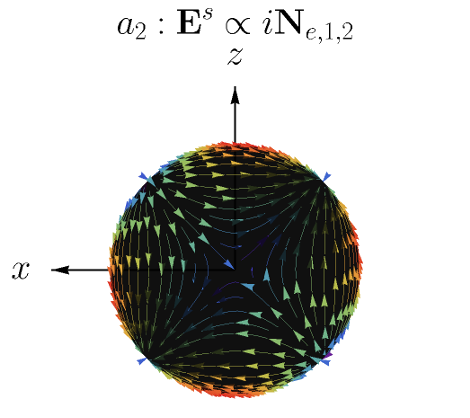
\includegraphics[scale=.25]{1-Teoria/figs/Ne12_static_crop.png}%
			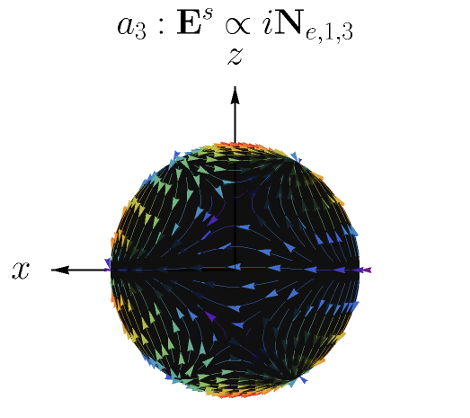
\includegraphics[scale=.25]{1-Teoria/figs/Ne13_static_crop.png}%
			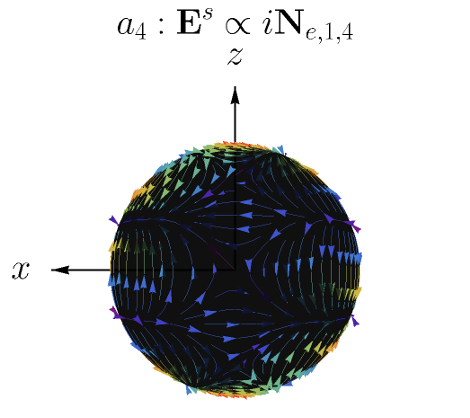
\includegraphics[scale=.25]{1-Teoria/figs/Ne14_static_crop.png}%
		\end{subfigure}\\
		\hspace{-4em}	
		\begin{subfigure}{.05\linewidth}\vspace{-3.25cm}\label{figs:MagneticMultipoles} \caption{ } \end{subfigure}
		\hspace{-3em}
		\begin{subfigure}{.9\linewidth}			
		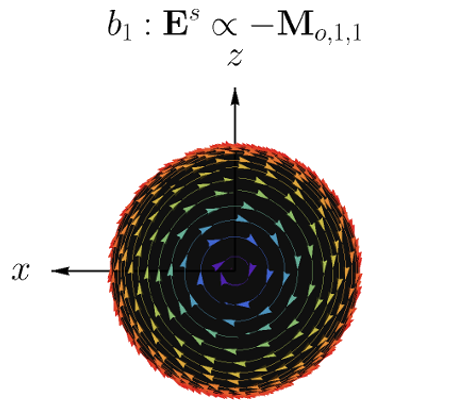
\includegraphics[scale=.25]{1-Teoria/figs/Mo11_static_crop.png}%
		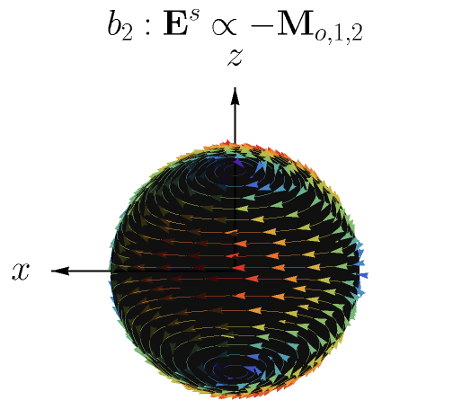
\includegraphics[scale=.25]{1-Teoria/figs/Mo12_static_crop.png}%
		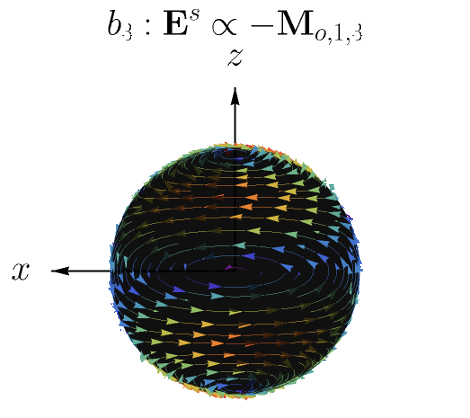
\includegraphics[scale=.25]{1-Teoria/figs/Mo13_static_crop.png}%
		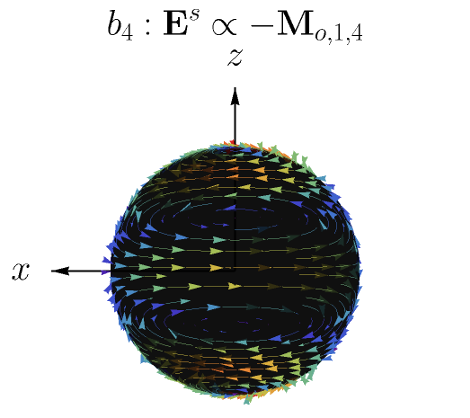
\includegraphics[scale=.25]{1-Teoria/figs/Mo14_static_crop.png}%
		\end{subfigure}
		\caption{Contribuciones multipolares \textbf{a)} eléctricas $a_\ell$ y \textbf{b)} magnéticas $b_\ell$ de orden $\ell = 1,2,3$ y $4$ del campo esparcido $\vb{E}^s$ por una partícula esférica, evaluadas en una superficie matemática esférica y concéntrica a la partícula que radía los campos EMs, en donde el plano de la página corresponde al plano de oscilación del campo eléctrico incidente $\vb{E}^i$. En las gráficas presentadas, el color rojo corresponde a los valores máximos del campo eléctrico, mientras que los rojos son los puntos menos intensos, donde se presentan los nodos en la superficie esférica.}
		\label{fig:Multipolos}
	\end{figure}

Los campos EMs esparcidos [Ecs. \eqref{eq:EHsAEV}] fueron calculados al considerar una onda plana incidente $\vb{E}^i$ polarizada en la dirección $x$ sin embargo, debido a la simetría de la esfera, una onda plana polarizada en la dirección $y$ se describe mediante la transformación $\varphi\to\varphi+\pi/2$, por lo que los campos EMs esparcidos y dentro de la esfera se calculan mediante el mismo procedimiento \cite{bohren1998absorption}. Entonces, cualquier cantidad relacionada con la absorción y esparcimiento de una esfera se calcula únicamente mediante lo coeficientes de Mie [Ecs. \eqref{eq:MieCoef}]. En particular, para determinar la matriz de esparcimiento $\mathbb{S}$ se relaciona el campos eléctrico esparcido en el límite de campo lejano, en donde al emplear las funciones de Ricatti-Bessel, y sus derivadas, en el límite asintótico\footnote{En el límite $\ell^2 \ll \rho$, se cumple que $h_\ell^{(1)}(\rho)\approx (-i)^\ell e^{i\rho}/i\rho$ y $\dv*{h_\ell^{(1)}}{\rho} = (-i)^\ell e^{i\rho}/\rho$. Por lo tanto,  $\xi(\rho)\approx (-i)^\ell e^{i\rho}/i$ y $\dv*{\xi}{\rho} = (-i)^\ell e^{i\rho}(1/i\rho + 1)$.} $\ell \ll kr$, las componentes radiales de los campos EMs decaen como $(kr)^{-2}$, por lo que es despreciable. Al escribir los armónicos esféricos  [Ecs. \eqref{eq:AEV}] en términos de $\pi_\ell$, $\tau_\ell$ y las funciones de Ricatti--Bessel $\psi$ y $\xi$ en el límite asintótico despreciando los términos proporcionales a $(kr)^{-1}$, el campo eléctrico esparcido en la componente paralela al plano de esparcimiento (ver Fig. \ref{fig:PlanoEsparcimiento}) es
	\begin{align*}
	E_\theta^s \vu{e}_\parallel^s &=\frac{\cos\varphi}{kr}
								\sum_\ell^\infty E_0i^\ell\frac{2\ell+1}{\ell(\ell+1)}
						(i a_\ell\xi_\ell'\tau_\ell-b_\ell\xi_\ell\pi_\ell)\vu{e}_\theta
			\approx E_0\cos\varphi\frac{e^{ikr}}{-ikr}\sum_\ell^\infty\frac{2\ell+1}{\ell(\ell+1)}
				( a_\ell \tau_\ell + b_\ell\pi_\ell )\vu{e}_\theta \\
		E_\varphi^s \vu{e}_\perp^s &= \frac{\sin\varphi}{kr}
							\sum_\ell^\infty E_0i^\ell\frac{2\ell+1}{\ell(\ell+1)}						
							(-ia_\ell\xi_\ell'\pi_\ell+b_\ell\xi_\ell\tau_\ell)\vu{e}_\varphi 
			\approx E_0\sin\varphi\frac{e^{ikr}}{-ikr}\sum_\ell^\infty\frac{2\ell+1}{\ell(\ell+1)}					(a_\ell\pi_\ell+b_\ell\tau_\ell)(-\vu{e}_\varphi)
	\end{align*}
donde $\vu{e}_\parallel^s =\vu{e}_\theta$ y $\vu{e}_\perp^s=-\vu{e}_\varphi$. Al emplear la Ec. \eqref{eq:EIncidente} para reescribir a la onda plana incidente $\vb{E}^i$ [Ec. \eqref{eqs:EiAEV}] en la base de $\{\vu{e}_\parallel^i,\vu{e}_\perp^i\}$ [Ec. \eqref{eq:vecInc}] se relaciona determina la forma explícita de la matriz de esparcimiento para una partícula esférica\vspace*{-.5em}
	\begin{tcolorbox}[title = Matriz de esparcimiento de Mie,  breakable ]
	\begin{align}
	\mqty(E_{\parallel}^s\\E_{\perp}^s)  =  
		\frac{e^{ik(r-z)}}{-ikr} \mqty(S_2 (\theta) & 0\\ 0 & S_1 (\theta))
	\mqty(E_{\parallel}^i\\E_{\perp}^i),	
	\label{eq:MieMatrix}
	\end{align}
	donde $E^i_\parallel=E_0\cos\varphi$, $E^i_\perp = E_0\sin\varphi$ y \begin{subequations}\\
	\eqhalf{	S_1 (\theta) = \sum_\ell^\infty\frac{2\ell+1}{\ell(\ell+1)}(a_\ell\pi_\ell+b_\ell\tau_\ell)
				\label{eqs:S_1}}
	\eqhalf{	S_2 (\theta) = \sum_\ell^\infty\frac{2\ell+1}{\ell(\ell+1)}( a_\ell \tau_\ell + b_\ell\pi_\ell )
			 \label{eqs:S_2}	}
	\label{eq:MatrixElements}	\end{subequations}
	\end{tcolorbox}\vspace*{-.5em}\noindent

\section{Respuesta electromagnética de materiales plasmónicos}

En el artículo original de Mie \cite{mie1908metallosung} se emplea la solución a los campos electromagnéticos (EMs) esparcidos para describir las propiedad ópticas de suspenciones coloidales de partículas esféricas de oro. En sus caĺculos, Mie asumió la  respuesta electromagnética (EM) del oro dada por los datos experimentales de la función dieléctrica $\varepsilon(\omega)$ del oro en bulto era válida también para nanopartículas (NPs) cuyo radio fuera al menos un orden de magnitud menor al de la longitud de onda de la luz que iluma a la NP \cite{horvath2009historic}. A pesar de que la suposición de Mie es válida para los cálculos que publicó \cite{horvath2009historic}, en general la respuesta electromagnética de los materiales depende de sus dimensiones y a la nanoescala los efecto de superficie toman relevancia respecto a los de bulto \cite{boverhof2015comparative}, por lo que la función dieléctrica de bulto debe corregirse para NPs. Para corregir la respuesta EM de NPs esféricas de materiales plasmónicos a partir de la función dieléctrica experimental de bulto, se emplea el modelo de Drude-Sommerfeld, el cual describe la función dieléctrica de un material en bulto con electrones de conducción a partir de asumir un gas de electrones libres \cite{gross2014festkorperphysik}. Al corregir el modelo de Drude-Sommerferd considerando los efectos de superficie de la NP e introducir esta corrección en los datos experimentales del bulto se construye una función dieléctrica apta para NPs y el cálculo de sus propiedades ópticas mediante la solución de Mie.

Para corregir la respuesta EM  en bulto de materiales plasmónicos, se asume que su función dieléctrica corresponde a la suma de la respuesta de la interacción de la radiación EM con los electrones de conducción del material  $\varepsilon^{inter}(\omega) $, correspondiente a las transiciones electrónicas interbanda, y con los electrones ligados  $\varepsilon^{intra}(\omega) $, correspondientes a las transiciones electrónicas intrabanda \cite{noguez2007surface}, es decir
	\begin{align*}
	\varepsilon^B_{exp}(\omega) = \varepsilon^{inter}(\omega) + \varepsilon^{intra}(\omega),
	\end{align*}
en donde $\varepsilon^B_{exp}(\omega)$ es la función dieléctrica de bulto que puede se medida de forma experimental \cite{johnson1972constants}. Para describir la contribución de los electrones de conducción en la respuesta EM del material $\varepsilon^{inter}(\omega)$ se emplea el modelo de Drude-Somerfeld que, desde un enfoque clásico, es la solución a la ecuación de movimiento de los electrones libres en un material ante la presencia de un campo eléctrico externo oscilante \cite{gross2014festkorperphysik}. El efecto de un campo eléctrico externo $\vb{E}$ sobre los electrones libres de un material es un cambio de su posición, por lo que aparecen momentos dipolares $\vb{p}=q_e\vb{r}$; con $q_e$, la carga del electrón y $\vb{r}$, su desplazamiento.  El efecto neto en el material es una polarización $\vb{P} = n_v \vb{p}$, donde $n_v$ es la densidad volumétrica electrónica \cite{novotny2006principles}.  La respuesta óptica del material dada por el modelo de Drude, caracterizada por la función dieléctrica $\varepsilon_D(\omega)$, depende de $\vb{E}$ y $\vb{P}$ como 
	\begin{align*}
	\vb{P} = \varepsilon_0\qty(\frac{\varepsilon_D}{\varepsilon_0}-1)\vb{E},
	\end{align*}
donde se asume que la polarización ocurre en la dirección del campo eléctrico \cite{novotny2006principles}.  Al reescribir  $\vb{P}$ como $n_v q_e \vb{r}$ se obtiene que
	\begin{align}
	n_v q_e \vb{r} = \varepsilon_0 \qty(\frac{\varepsilon_D}{\varepsilon_0}-1)\vb{E}. 
	\label{eq:PolarizationDrude}
	\end{align}
Si el material se encuentra ante la presencia de un campo eléctrico oscilante de la forma $\vb{E}_0 e^{-i\omega t}$, la ecuación de movimiento que obedece un electrón libre del material es \cite{kreibig1995clusters,gross2014festkorperphysik}
	\begin{align}
	m_e^* \pdv[2]{\vb{r}}{t} +  \gamma \pdv{\vb{r}}{t} = q_e\vb{E}_0e^{-i\omega t},
	\label{eq:movementDrude}
	\end{align}
donde $m_e^*$ es la masa efectiva del electrón\footnote{La masa efectiva es el resultado de la interacción de un electrón con el potencial de la red cristalina que conforma al material, los fonones de la red y con los otros electrones en la red \cite{gross2014festkorperphysik}. } \cite{gross2014festkorperphysik} y $\gamma$ es la \emph{constante fenomenológica de amortiguamiento} \cite{kreibig1995clusters}, que es el inverso del tiempo promedio entre eventos de colisiones  de los electrones \cite{novotny2006principles,gross2014festkorperphysik}.  Al multiplicar la Ec.  \eqref{eq:movementDrude} por $n_v q_e$, resolverla con el \emph{Ansatz} $\vb{r} = \vb{r}_0e^{-i\omega t}$ y compararla con la Ec.  \eqref{eq:PolarizationDrude}, se obtiene la función dieléctrica \cite{novotny2006principles,gross2014festkorperphysik}  \vspace*{-.5em}
	\begin{tcolorbox}[title = Modelo de Drude-Sommerfeld, breakable ]
	\eqhalf{\frac{\varepsilon_D(\omega)}{\varepsilon_0}= 1 - \frac{\omega_p^2}{\omega(\omega+i\gamma)},
	\label{eq:Drude}}
	\eqhalf{	\omega_p =\sqrt{ \frac{n_v e^2}{m_e^* \varepsilon_0}}.
	\label{eq:wp}}
	\end{tcolorbox}\vspace*{-.5em}\noindent
con $\omega_p$, la frecuancia de plasma.

Dado que la constante fenomenológica $\gamma$ depende de la geometría del material, se emplea en la Ec. \eqref{eq:Drude} la constante fenomenológica de bulto $\gamma_\infty$ dada por \cite{kreibig1995clusters}
	\begin{align}
	\gamma_\infty = \frac{v_F}{L}
			 \label{eq:gammaInf}	
	\end{align}
donde $v_F$ es la velocidad de Fermi\footnote{En un sistema con $N$ electrones, que obedecen el principio  de exclusión de Pauli, la energía de Fermi $E_F$ es la máxima ocupada, dada por $E_F = (\hbar^2/2m_e^*)k_F^2$, con $k_F$, la norma del vector de onda de Fermi \cite{gross2014festkorperphysik}.  Puesto que la velocidad de Fermi es $v_F = p_F/m_e^* = \hbar k_F / m$ y que para un gas de electrones libres $k_F=(3\pi n_v)^{1/3}$, se obtiene que para metales típicos $v_F\approx 10^{15}$ nm s$^{-1}$ \cite{gross2014festkorperphysik}. } del material a una temperatura dada y $L$ es el camino libre medio, que representa la distancia promedio que recorren los electrones entre eventos de colisiones \cite{gross2014festkorperphysik}.  

La frecuencia de plasma $\omega_p$ en el modelo de Drude-Sommerfeld delimita regímenes donde el material plasmónico se comporta como un metal o como un dieléctrico \cite{trugler2011properties}.   En la Fig.  \ref{fig:Drude} se muestran las funciones dieléctricas (gráfica interna) y los índices de refracción  (gráfica principal) modelados por una función tipo Drude con $\omega_p=4. 3$ eV [Fig.  \ref{sfig:Drude4eV}] y $10$ eV [Fig.  \ref{sfig:Drude10eV}], y $\gamma=0. 15$ eV.  En estas gráficas se observa que $\Re[\varepsilon(\omega)]<0$ para $\omega<\omega_p$, por lo que al sustituir el índice de refracción en la expresión de una onda plana propagante se obtiene una onda evanescente, es decir, la onda plana no penetra el material y es reflejada: el material presenta una respuesta metálica.  Para $\omega>\omega_p$, se cumple que $\Re[\varepsilon(\omega)]>0$ y $\Im[\varepsilon(\omega)]\approx 0$, por lo que el índice de refracción, en dicho régimen, se comporta como el de un  material transparente. 

	\begin{figure}[h!]\centering\hspace*{-1.5em}
	\begin{subfigure}{.01\linewidth}\caption{}\label{sfig:Drude4eV}\vspace{3.75cm}\end{subfigure}
	\begin{subfigure}{.45\linewidth}\hspace*{-1.3em}
	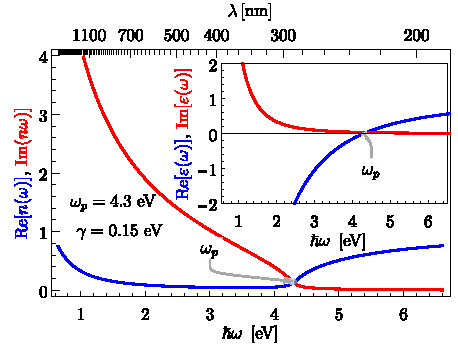
\includegraphics[scale=1]{1-Teoria/figs/1-4-varepsn4eV.pdf}
	\end{subfigure}
	\begin{subfigure}{.01\linewidth}\caption{}\label{sfig:Drude10eV}\vspace{3.75cm}\end{subfigure}
	\begin{subfigure}{.45\linewidth}\hspace*{-1em}
	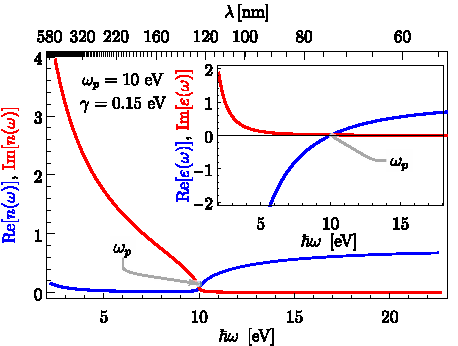
\includegraphics[scale=1 ]{1-Teoria/figs/1-4-varepsn10eV.pdf}
	\end{subfigure}\vspace*{-.7em}
	\caption{ Índice de refracción (gráfica externa) y función dieléctrica (gráfica interna) del modelo de Drude-Sommerfeld para las frecuencias de plasma \textbf{a)} $\omega_p=4. 3$ eV y \textbf{b)} $\omega_p=10$ eV; ambos casos con $\gamma=0. 15$ eV, como función de la energía.  En el marco superior se observa su dependencia en longitud de onda $\lambda$. }\label{fig:Drude}
	\end{figure}	


\subsection{Corrección por tamaño para partículas esféricas}

Para corregir la función dieléctrica de bulto obtenida mediante métodos experimentales $\varepsilon_B^{exp}(\omega)$ se modifica la constante fenomenológica  en el modelo de Drude-Sommerfeld\footnote{También es posible hacer una corrección de tamaño en la contribución interbanda de la función dieléctrica sin embargo, para los datos experimentales de \cite{johnson1972constants}, la corrección para partículas esféricas es apreciable para NPs con radios menores a $2$ nm \cite{mendoza2014determination}.} dado que ésta depende del camino libre medio de los electrones $L$ y debe modificarse cuando el radio de las NPs $a$ es menor a $L$ \cite{kreibig1995clusters}. Por ejemplo, para metales típicos, como el oro y la plata, a frecuencias del espectro visible y a una temperatura de $273$ K, el camino libre medio de los electrones es  de $56$ nm para el oro y $42$ nm para la plata\footnote{Cálculos a partir de los datos obtenidos de \cite{ashcroft1976solid}.}, por lo que para NPs de oro o plata con radios menores a $60$ nm se hace una corrección de la constante fenomenológica para materiales de bulto. La corrección de $\gamma_\infty$ para una partícula esférica de radio $a$ se calcula al considedar el camino libre medio efectivo de los electrones, proporcional al radio de la partícula, obteniedo así un término de amortiguamiento adicional al de bulto y que es aditivo a éste \cite{kreibig1995clusters}, es decir,
	\begin{align*}
	 \gamma = \gamma_\infty + \gamma_a = v_F \qty(\frac{1}{L}+\frac{A}{a}). 
	\end{align*}
donde $A$ es un parámetro del orden de la unidad \cite{noguez2007surface,mendoza2014determination} y depende de la teoría con la que sea cálculado el camino libro medio efectica \cite{kreibig1995clusters}.  Entonces, para NPs esféricas modeladas por una función dieléctrica tipo Drude [Ec.  \eqref{eq:Drude}] se emplea  la corrección por tamaño de la función dieléctrica dada por
	\begin{align}
	\frac{\varepsilon(\omega)}{\varepsilon_0} = \frac{\varepsilon_B^{exp}(\omega)}{\varepsilon_0}
						 - \qty( 1 - \frac{\omega_p^2}{\omega(\omega+i\gamma_\infty)}) 
						 + \qty( 1 - \frac{\omega_p^2}{\omega[\omega+i(\gamma_\infty + v_F A/a)]})
	\end{align}
en donde se resta la contribución del material de bulto  a la función dieléctrica experimental $ \varepsilon_B^{exp}(\omega)$ y se introduce la función dieléctrica con la corrección $\gamma = \gamma_\infty+\gamma_a$. Para realizar este proceso se debe encontrar los parámetros $\omega_p$ y $\gamma_\infty$ que mejor ajusten al modelo de Drude sin embargo, la función dieléctrica experimental del material $\varepsilon_B^{exp}(\omega)$ depende del método de fabricación de la muestra, del sustraso sobre el que está puesta, además de que  los valores de los parámetros de la función dieléctrica tipo Drude cambian de valor según sea el método empleado para su cálculo \cite{svetovoy2008optical}.  Asimismo, la función dieléctrica experimental presenta contribuciones no plasmónicas que no son descritas por Drude apreciables a energías $\hbar\omega$ más altas que las transiciones interbanda, por lo que el ajuste debe realizarse hasta un valor de $\omega$ que ya no siga las tendencias del modelo de Drude \cite{mendoza2014determination}.

Para determinar los parámetros $\omega_p$ y $\gamma$ del modelo de Drude [Ec. \eqref{eq:Drude}] se emplea el método propuesto es \cite{mendoza2014determination}, donde se relaciona $\varepsilon' = \Re[\varepsilon_D(\omega)/\varepsilon_0]$ con $\varepsilon''=\Im[\varepsilon_D(\omega)/\varepsilon_0]$ a partir de dos relaciones lineales. Las partes real e imaginaria de la Ec. \eqref{eq:Drude} son \begin{subequations}

	\eqhalf{\varepsilon' =
		 1 - \frac{\omega_p^2 \omega^2}{\omega^4 + (\omega\gamma)^2},
		 \label{eqs:ReDrude}}
	\eqhalf{\varepsilon'' =
		 \frac{\omega_p^2  (\omega\gamma)}{\omega^4 + (\omega\gamma)^2}.
		 \label{eqs:ImDrude}
			}\end{subequations} \noindent

Dado que $1-\varepsilon' = \omega_p^2\omega^2 / [\omega^4 + (\omega\gamma)^2]$, al calcular  $(1-\varepsilon')\gamma/\omega$ y sustituir con la Ec. \eqref{eqs:ImDrude} se obtiene que $	( 1-\varepsilon') \frac{\gamma}{\omega} =\varepsilon''$, por lo que se cumple la relación
	\begin{align}
	\omega\varepsilon''= \gamma( 1-\varepsilon') \label{eq:gammaAjuste}
	\end{align}
Asimismo, al calcular la suma del cuadrado de $1-\varepsilon'$ y el cuadrado de $\varepsilon''$ se obtiene
	\begin{align*}
	( 1-\varepsilon') ^2 + (\varepsilon'')^2 
					&=\frac{\omega_p^4 \omega^4}{[\omega^4 + (\omega\gamma)^2]^2}+
									\frac{\omega_p^4 (\omega\gamma)^2}{[\omega^4 + (\omega\gamma)^2]^2}\\
					&= \frac{\omega_p^4[\omega^4 + (\omega\gamma)^2]}{[\omega^4 + (\omega\gamma)^2]^2}\\
					&= \frac{\omega_p^4}{\omega^4 + (\omega\gamma)^2},
		\end{align*}
y al multiplicar ambos lados de la ecuación por $\omega^2$	 y sustituir con la Ec. \eqref{eqs:ReDrude} se obtiene
	\begin{align}
	\omega^2\qty[( 1-\varepsilon') ^2 + (\varepsilon'')^2 ]  
						= \omega_p^2( 1-\varepsilon').
	\label{eq:omegaAjuste}
	\end{align}
Es decir, al graficar las Ecs. (6) y (7) como función de $ 1-\Re[\varepsilon(\omega)] $ se obtienen dos funciones lineales sin ordenada al origen por lo que, al emplear los valores experimentales de la función dieléctrica, cuando estos no correspondan a una recta que cruza por el origen, la funciín dieléctrica deja de ser modelada por el modelo de Drude. Asimismo, es posible determinad los parámetros $\omega_p$ y $\gamma$ de la función dieléctrica empleando los valores de la parte real y la parte imaginario de $\varepsilon(\omega)$ es decir, considerando ambas contribuciones. Las funciones a ajustar son




	\begin{figure}[t!]\centering\hspace*{-1.5em}
	\begin{subfigure}{.01\linewidth}\caption{}\label{sfig:Drude4eV}\vspace{3.75cm}\end{subfigure}
	\begin{subfigure}{.45\linewidth}\hspace*{-1.3em}
	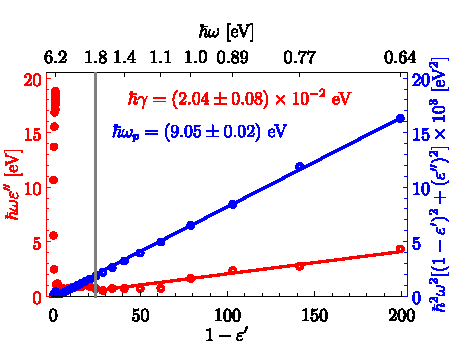
\includegraphics[scale=1]{1-Teoria/figs/1-4-DrudeFit_Ag.pdf}
	\end{subfigure}
	\begin{subfigure}{.01\linewidth}\caption{}\label{sfig:Drude10eV}\vspace{3.75cm}\end{subfigure}
	\begin{subfigure}{.45\linewidth}\hspace*{-1em}
	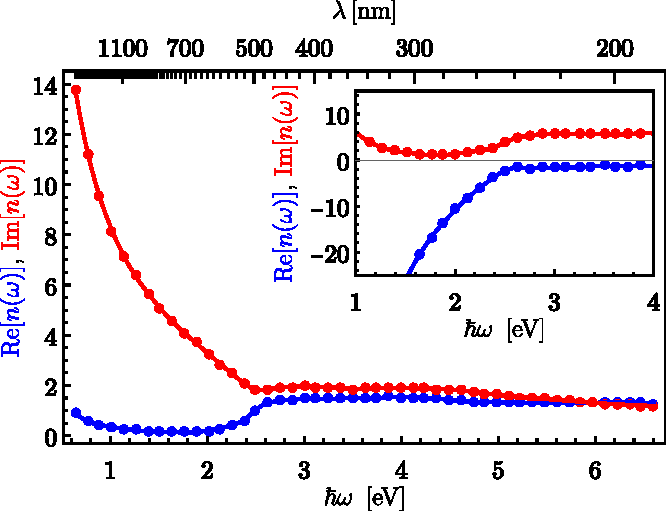
\includegraphics[scale=.6]{1-Teoria/figs/1-4-varepsn_JC_Au.pdf}
	\end{subfigure}\vspace*{-.7em}
	\caption{ Índice de refracción (gráfica externa) y función dieléctrica (gráfica interna) del modelo de Drude-Sommerfeld para las frecuencias de plasma \textbf{a)} $\omega_p=4. 3$ eV y \textbf{b)} $\omega_p=10$ eV; ambos casos con $\gamma=0. 15$ eV, como función de la energía.  En el marco superior se observa su dependencia en longitud de onda $\lambda$. }\label{fig:Drude}
	\end{figure}	








En la Fig.  \ref{fig:nJC} se muestran los resultados experimentales para el índice de refracción de bulto del oro [Fig.  \ref{sfig:nAuJC}] y de la plata [Fig.  \ref{sfig:nAgJC}], obtenidos de  \cite{johnson1972constants}.  Los datos experimentales muestran una respuesta cualitativa semejante al modelo de Drude-Sommerfeld (Fig.  \ref{fig:Drude}) para energías bajas: energías menores a $2. 50$ eV para el oro y menores a $3. 5$ eV para la plata. % En las regiones de mayor energía, la parte imaginaria del ínidice de refracción no tiende a cero, como sí lo hace en el modelo de Drude-Sommerfeld. 

%\begin{figure}[b!]\centering
%	\begin{subfigure}{.01\linewidth}\caption{}\label{sfig:nAuJC}\vspace{3.7cm}\end{subfigure}\hspace*{-1em}
%	\begin{subfigure}{.46\linewidth}\centering 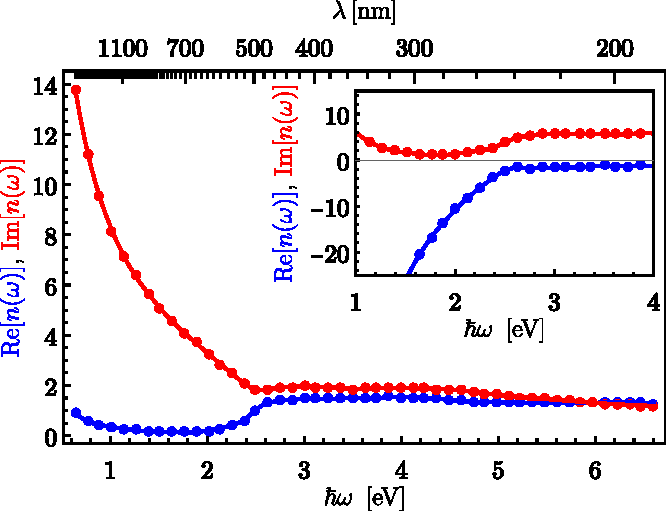
\includegraphics[scale=.7]{1-Teoria/figs/1-4-varepsn_JC_Au.pdf}\end{subfigure}
%	\begin{subfigure}{.01\linewidth}\caption{}\label{sfig:nAgJC}\vspace{3.7cm}\end{subfigure}\hspace*{-.8em}
%	\begin{subfigure}{.45\linewidth}\centering 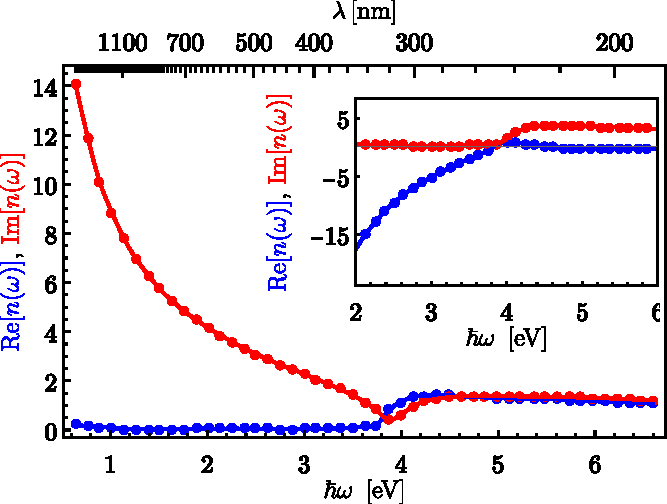
\includegraphics[scale=.7]{1-Teoria/figs/1-4-varepsn_JC_Ag.pdf}\end{subfigure}\vspace*{-.5em}
%	\caption{ Gráficas del índice de refracción (gráfica externa) y de la función dieléctrica (gráfica interna)  \textbf{a)} del oro y \textbf{b)} de la plata,  como función de la energía.  En el marco superior se observa su dependencia en longitud de onda $\lambda$.  Los puntos en ambas gráficas corresponden a los datos experimentales obtenidos de \cite{johnson1972constants} y las líneas continuas son sólo una ayuda visual al lector. }\label{fig:nJC}
%	\end{figure}	



\subsection{Plasmones}

En la deducción de la función dieléctrica del modelo de Drude [Ec. \eqref{eq:Drude}] se resolvió la ecuación de movimiento de los electrones libres en un material ante la  presencia de un campo eléctrico oscilante en el tiempo. A las oscilaciones colectivas  de los electrones dentro del material debido al acoplamiento con la radiación EM se les denominan  plasmones y estos ocurren a  frecuencias $\omega$ específicas \cite{stockman2011nanoplasmonics}. Para determinar a qué frecuencias se excitan los plasmones se calcula el rotacional de la ley de Faraday-Lenz y se sustituye con la ley de Ampère-Maxwell, tras calcular su transformada de Fourier el resultado obtenido es \cite{maier2007plasmonics}
	\begin{align*}
	\vb{k}(\vb{k}\cdot\vb{E})-k^2\vb{E} =
			 -\frac{\varepsilon(\omega)}{\varepsilon_0}
			 \frac{\omega^2}{c^2}\vb{E},
	\end{align*}
donde se hace la distinción entre los casos de ondas transversales ($\vb{k}\cdot\vb{E}=0$), en donde se cumple \vspace*{-.5em}
	\begin{tcolorbox}[title = Relación de dispersión genérica, ams align, breakable ]
	k^2 = \frac{\varepsilon(\omega)}{\varepsilon_0}  \frac{\omega^2}{c^2},
	\label{eq:TMode}
	\end{tcolorbox}\vspace*{-.5em}\noindent
y los casos con ondas longitudinales ($\vb{k}\cdot\vb{E}=kE$), en donde
	\begin{align}
	\varepsilon(\omega) = 0.
	\label{eq:LMode}
	\end{align}
Al sustituir con la función dieléctrica dada por el modelo de Drude-Sommerfeld [Ec. \eqref{eq:Drude}] en el límite $\gamma\ll\omega$ en las Ecs. \eqref{eq:TMode} y \eqref{eq:LMode} se obtiene \vspace*{-.5em}
	\begin{tcolorbox}[title = Relación de dispersión del plasmón de volumen,  breakable ]
para el modo longitudinal 
	\begin{align}
	\omega=\omega_p,
	\end{align}
y para el modo transversal 
	\begin{align}
		\omega =  \sqrt{(ck)^2+\omega_p^2},
	\label{eq:volumePlasmon}
	\end{align}
	\end{tcolorbox}\vspace*{-.5em}\noindent
Dado que el plasmón de volumen es un modo longitudinal no puede acoplarse a ondas EMs transversales por lo que sólo puede ser excitado mediante el impacto de partículas \cite{maier2007plasmonics}. Sin embargo, existen otro tipo de excitaciones que sí responden a ondas EM transversales; uno de los casos es cuando se tiene una interfaz plana entre un medio dieléctrico y uno metálico y es denominado plasmón polaritón de superficie (Surface Plasmon Polariton, SPP).
	

\begin{figure}[h!]\centering
	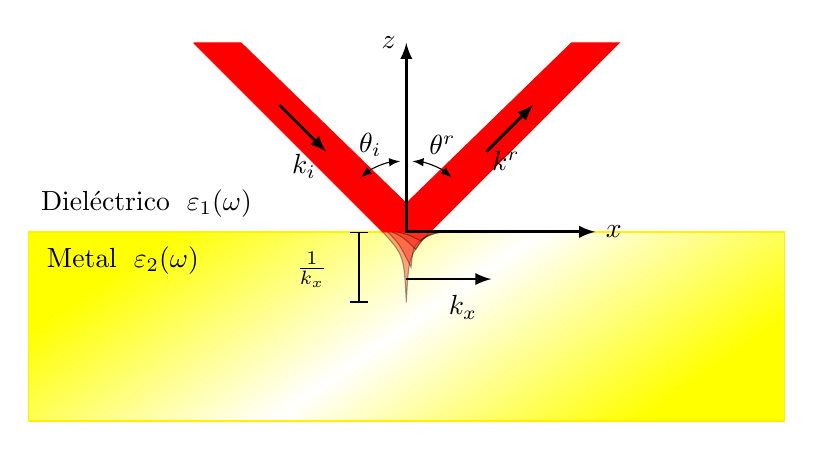
\begin{tikzpicture}[scale=1.2]
	%-------------------------------------------- Incidence media
\shadedraw[	top color = yellow,				%%%%	Color de arriba
			bottom color =yellow,				%%%%	Color de abajo
			middle color = white, 			%%	Color de en medio
			shading angle = 35]			%%%%	Ángulo de gradiente
		 (-4,-2) rectangle (4,0);
% Interface
\draw[yellow,line width=.5pt](-4,0)--(4,0)--(4,-2)--(-4,-2)--(-4,0); %%..5pt, interface]
% Media names
\node at (-2.75,.3) {Diel\'ectrico $\; \varepsilon_1(\omega)$}; 
\node at (-3,-.3) {Metal  $\; \varepsilon_2(\omega)$};

%-------------------------------------------- Laser beam outside
\draw[fill=red, opacity = 1,red](-2.25,2)--(-1.75,2)-- (0,.3)  %%% outside the metal
						--(1.75,2)--(2.25,2)
						--(.25,0)--(-.25,0)--(-2.25,2);																														
%--------------------------------------------  Incident Wave
\path (0,0)++(112.5:1cm)node{$\theta_i$};       % Angle
\draw[latex - latex](95:.75cm)arc(95:130:.75cm);
 
    \draw[- latex,line width=1pt](135:1.9cm)--(135:1.2cm);    %Wave vector
    \path (0,0)++(141:1.1cm)node[left]{$\vb{k}_i$};     %Wave vector label
    
%--------------------------------------------  Reflected Wave
\path (0,0)++(67.5:1cm)node{$\theta^r$};       % Angle
\draw[latex - latex](85:.75cm)arc(85:50:.75cm);
 
    \draw[- latex,line width=1pt](45:1.2cm)--(45:1.9cm);    %Wave vector
    \path (0,0)++(43:1.1cm)node[right]{$\vb{k}^r$};     %Wave vector label
  
%--------------------------------------------  Transmitted Wave & Skin depth
\draw[fill = red, opacity = .35] (-.25,0) ..controls (-.025,-.25) .. (0,-.75)
											..controls (.025,-.25) .. (.25,0);  %1st evanescent wave
\draw[fill = red, opacity = .35] (-.2,0) ..controls (-.075,-.125) .. (0.05,-.375)
											..controls (.075,-.125) .. (.3,0);  %2nd evanescent wave
\draw[fill = red, opacity = .35] (-.15,0) ..controls (-.025,-.0625) .. (0.1,-.1875)
											..controls (.175,-.0625) .. (.35,0);  %3rd evanescent wave
\draw[fill = red, opacity = .35] (-.1,0) ..controls (.025,-.03125) .. (0.15,-.09375)
											..controls (.225,-.03125) .. (.4,0);  %4th evanescent wave	

    \draw[- latex,line width=1pt](0,-.5)--(.9,-.5);    %Wave vector
    \node at (.6,-.8) {$\vb{k}_x$};
    
    \draw[|-|,line width=.2mm,black] (-.5,.0)--(-.5,-.75);%
    \node at (-1,-.4) {$\frac{1}{k_x}$};
%--------------------------------------------  Axes
\draw[latex - latex, line width =1pt] (0,2)node[left]{$z$}--(0,0) -- (2,0)node[right]{$x$};
\end{tikzpicture}
	\caption{ Esquema de la interfaz entre un medio dieléctrico y un medio metálico; ambos homogéneos, lineales e isótropos. Un haz de luz incide en el metal desde el medio dieléctrico.  La reflexión es total debido a la naturaleza metálica del material sin embargo, se presenta una onda evanescente que se propaga en dirección paralela a la interfaz.}\label{fig:SPP}
	\end{figure}
	
	La caracterización de los SSP se hace a través de su relación de dispersión, que puede ser calculada al considerar la geometría presentada en la Fig. \ref{fig:SPP}, en la cual se asume que la función dieléctrica es $\varepsilon(z,\omega)$, tal que  es $\varepsilon_1(\omega)>0$  la de un medio dieléctrico para $z>0$, y  $\varepsilon_2(\omega)$  para $z<0$ , la de un medio metálico que cumple con la propiedad que  $\Re[\varepsilon_2(\omega)]<0$, que en el modelo de Drude-Sommerfeld [Ec. \eqref{eq:Drude}] basta con $\omega<\omega_p$.  Por la naturaleza metálica del material, en la interfaz se encuentran ondas EMs evanescentes que, por simplicidad, se asume la dirección $x$ como dirección de propagación, por tanto, se pueden escribir los campos EMs como

	\begin{subequations}\eqhalf{	\vb{E}(\vb{r},t) = \vb{E}(z)e^{ik_x x-\omega t },}
	\eqhalf{\vb{H}(\vb{r},t) = \vb{H}(z)e^{ik_x x-\omega t},}
	\label{eq:EHbetax}\end{subequations} 
	
\noindent con $k_x$ la componente paralela a la interfaz del vector de onda. Si $z>0$, entonces $\vb{E}(z)=\vb{E}_1$, con $E_1$ la magnitud de del campo eléctrico dentro del dieléctrico, y si $z<0$, entonces $\vb{E}(z)=\vb{E}_2$, la magnitud de del campo eléctrico en el medio metálico; la misma distinción se hace para el campo $\vb{H}$. Dado que los campos EMs cumplen con la ecuación de Helmholtz [Ec. \eqref{eq:Helmholtz}], al sustituir las expresiones de las Ecs. \eqref{eq:EHbetax}, se obtiene

	\begin{subequations}
	\eqhalf{	\pdv[2]{\vb{E}}{z} + \qty[k_0^2\frac{\varepsilon(z)}{\varepsilon_0} - k_x^2 ] \vb{E}= 0,\label{eq:helmE}}
	\eqhalf{\pdv[2]{\vb{H}}{z} + \qty[k_0^2\frac{\varepsilon(z)}{\varepsilon_0}  - k_x^2 ] \vb{H}= 0, \label{eq:helmH}}
	\end{subequations} 
	
\noindent en donde $k_0 = \omega/c$.	La polarización de la onda plana incidente interviene en la relación de dispersión del SPP, por lo que se calcularan los los campos EMs para las polarizaciones \emph{s} y \emph{p}. Se considera, además, que  hay homogeneidad en la dirección $y$ y que la única dependencia en la variable $x$  es en el término de propagación, es decir, que $\partial/\partial x\to ik_x$. Bajo estas consideraciones, al desarrollar la ley de Faraday-Lenz y la ley de Ampère-Maxwell con las expresiones de las Ecs. \eqref{eq:EHbetax} se obtiene el conjunto de ecuaciones

	\begin{subequations}
	\eqhalf{	\mqty(-\pdv*{E_y}{z} \\ \pdv*{E_x}{z}-ik_x E_z\\ik_x E_y)
				= i\omega\mu_0 \mqty(H_x\\H_y\\h_z),}
	\eqhalf{	\mqty(-\pdv*{H_y}{z} \\ \pdv*{H_x}{z}-ik_x H_z\\ik_x H_y)
				= i\omega\varepsilon(z) \mqty(E_x\\E_y\\E_z).}	
	\end{subequations} 

En la configuración de polarización \emph{s}, las componentes no nulas de los campos EM son $E_y$, $H_z$ y $H_x$, por los campos EMs cumplen con las relaciones

	\begin{subequations}
	\eqhalf{	H_x =  \frac{i}{\omega \mu_0} \pdv{E_y}{z},\label{eq:Hx}}
	\eqhalf{H_z =  \frac{q}{\omega \mu_0} E_y, \label{eq:Hz}}	
	\label{eq:ondaS}	\end{subequations} 

\noindent además de la Ec. \eqref{eq:helmE} con $\vb{E} = E_y\vu{e}_y$, cuya solución se propone como
	\begin{subequations}
	\begin{align}
	E_y(z) = \begin{dcases}
		E_1 e^{ik_x x} e^{-k_{1,z}z}, & z>0,\\
		E_2 e^{ik_x x} e^{k_{2,z} z}, & z<0,
		\end{dcases}\label{eqs:AnsatzEy}
	\end{align}
con $k_{j,z} = k_j\cos\theta_i$ y $k_j = k_0 \sqrt{\varepsilon_j(\omega)/\varepsilon_0}$, con $j = 1,2$; donde se escribe de forma explícita el comportamiento de decaimiento exponencial en la amplitud y se omite el término $e^{-i\omega t}$ por simplicidad. Se impone que $\Re[\sqrt{\varepsilon_j(\omega)}] >0$, para que la amplitud de los campos EM ---y por tanto la energía--- sea una cantidad acotada. Al calcular el campo $\vb{H}$ con las Ecs. \eqref{eq:ondaS} y \eqref{eqs:AnsatzEy}, se obtienen a las expresiones 
	
	\eqhalf{	H_x(z) = \begin{dcases}
	-i \frac{E_1}{\omega\mu_0}k_{1,z} e^{ik_x x} e^{-k^1_z 	z}, & z>0,\\
	i \frac{E_2}{\omega\mu_0}k_{2,z} e^{ik_x x} e^{k^2_z z}, & z<0,
	\end{dcases}}
	\eqhalf{	H_z(z) = \begin{dcases}
	\frac{E_1}{\omega\mu_0}k_x  e^{ik_x x} e^{k_{1,z} z} & z>0,\\
	\frac{E_2 }{\omega\mu_0}k_x  e^{ik_x x} e^{k_{2,z}z} & z<0.
	\end{dcases}}\label{eqs:EyHxHz}\end{subequations}
	
\noindent   Las condiciones a la frontera de los campos EMs imponen que la componente paralela a la interfaz del campo eléctrico, $E_y$, sea continua, por lo que $E_1 = E_2$. Adicionalmente, por la ausencia de corrientes externas y dado que ambos medios son no magnéticos, las componentes perpendiculares del campo $\vb{H}$ son igualmente continuas. Entonces, a partir de las Ecs. \eqref{eqs:EyHxHz} se concluye que

	\begin{align}
	E_1\qty(k_{1,z}+k_{2,z})= E_1 k_0\cos\theta_i \qty[\sqrt{\frac{\varepsilon_1}{\varepsilon_0}} + \sqrt{\frac{\varepsilon_2}{\varepsilon_0}}] = 0. \label{eq:condS}
	\end{align}
	
\noindent Por el \emph{Ansatz} propuesto en la Ec. \eqref{eqs:AnsatzEy}, la parte real de la raiz cuadrada de ambas funciones dieléctricas son mayores a cero, por tanto, la Ec. \eqref{eq:condS} se satisface si $E_1 = E_2 = 0$, es decir  que no existe un acoplamiento entre los electrones libres del metal en la interfaz plana y la onda EM incidente para polarización \emph{s}.

El cálculo de la relación de dispersión del SPP cuando incide una onda plana con polarización \emph{p} es análogo al cálculo con polarización \emph{s} al intercambiar el campo eléctrico por el campo $\vb{H}$ y al intercambiar la permitividad magnética por la función dieléctrica, es decir, $\vb{E}\leftrightarrow\vb{H}$ y $\varepsilon(z)\leftrightarrow\mu_0$. Al considerar las condiciones de continuidad del campo $\varepsilon(z)\vb{E}$ y el campo $\vb{H}$ se llega a la condición
	\begin{align}
	\frac{k_{1,z}}{k_{2,z}} = - \frac{\varepsilon_1}{\varepsilon_2}. \label{eq:condP}
	\end{align}
Por el \emph{Ansatz} propuesto en la Ec. \eqref{eqs:AnsatzEy}, se impone que $\Re[\sqrt{\varepsilon_j(\omega)}] >0$,  por lo tanto, en la Ec. \eqref{eq:condP}  la parte real de las permitividades eléctricas de ambos materiales deben ser de signo opuesto, es decir, el acoplamiento de los electrones libres en la interfaz sólo ocurre entre un medio dieléctrico y uno metálico. Asimismo, la ecuación de Helmholtz para el campo $\vb{H}$ [Ec. \eqref{eq:helmH}] impone que
	\begin{align}
	k_{j,z}^2 = k_x^2 - k_0^2 \frac{\varepsilon_j}{\varepsilon_0}.
	\label{eq:kdkm}
	\end{align}
Al elevar al cuadrado la Ec. \eqref{eq:condP}, sustituir con la Ec. \eqref{eq:kdkm}, y  despejar $k_x$  empleando la identidad de diferencia de cuadrados,  se calcula la relación de dispersión de SSP. Adicionalmente, como  $k_0^2 \varepsilon_j(\omega)= k_x^2 +k_{j,z}^2$, entonces $k_{j,z}= \sqrt{k_0^2 \varepsilon_j(\omega)- k_x^2}  $, por lo que \vspace*{-.5em}\begin{subequations}
	\begin{tcolorbox}[title = Relación de dispersión del SPP, breakable ]
	\eqhalf{k_x^2 = \frac{k_0^2}{\varepsilon_0} \frac{\varepsilon_1 \varepsilon_2}{\varepsilon_1 + \varepsilon_2},
	\label{eq:kx}}
	\eqhalf{	k_{j,z}^2 = \frac{k_0^2}{\varepsilon_0} \frac{\varepsilon_j^2}{\varepsilon_1 + \varepsilon_2},}
	
	con $j=1$ es el medio dieléctrico y $j=2$ es el medio metálico.
	\end{tcolorbox}\end{subequations}\vspace*{-.5em}\noindent

La frecuencia de resonancia $\omega$ del SPP se encuentra cuando al Ec. \eqref{eq:kx} es máxima, es decir, cuando $\varepsilon_1(\omega)+\varepsilon_2(\omega)$ es mínima. Si se emplea el modelo de Drude-Sommerfeld [Ec. \eqref{eq:Drude}] en el límite $\gamma\ll\omega$, entonces  \vspace*{-.5em}
	\begin{tcolorbox}[title =Frecuencia de resonancia del SPP, ams align,  breakable ]
	\omega = \frac{\omega_p}{\sqrt{1+\varepsilon_1/\varepsilon_0}}
	\end{tcolorbox}\vspace*{-.5em}\noindent

	
	
	
	
	\begin{figure}[h!]\centering
		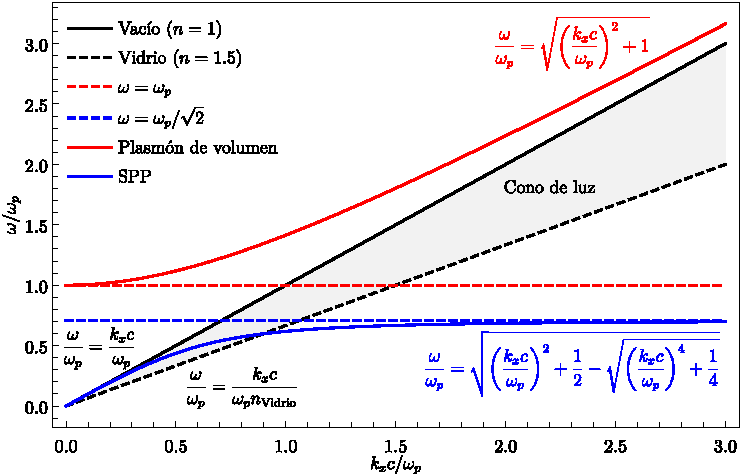
\includegraphics[scale=1]{1-Teoria/figs/1-4-RelacionDispersion.pdf}\vspace*{-1em}
	\caption{Frecuencias de resonancia $\omega_\ell/\omega_p$ para una esfera con una función dieléctrica tipo Drude, como función del parámetro adimensional  $\omega_p a / c$, para los multipolos $\ell = 1,2,3$ y $4$. }
	\label{fig:NormalModes}
	\end{figure}		
	
	
	
	
	

 frecuencias donde ocurren las SPRs \cite{stockman2011nanoplasmonics}.  La clasificación de los plasmones comprende  dos tipos: propagantes y localizados.  Cuando los plasmones se propagan a lo largo de una interfaz plana entre un medio diel\'ectrico y uno met\'alico se denomina  \emph{plasm\'on-polarit\'on de superficie} (Surface Plasmon Polariton, SPP) \cite{maier2007plasmonics}.  Si el plasmón, en cambio, se encuentra en la superficie de una partícula  met\'alica, de tamaño finito, se le conoce como \emph{resonancia de plasm\'on de superficie localizado} (Localized Surface Plasmon Resonance, LSPR) \cite{maier2007plasmonics}. 













	El campo esparcido [Ec.  \eqref{eq:Es}] está en términos de los coeficientes $a_\ell$ y $b_\ell$ [Ecs.  \eqref{eq:MieCoef}], que dependen, entre otros parámetros, del índice de refracción de la partícula.  De la Ec.  \eqref{eq:Es} se observa que, para un multipolo $\ell$ fijo, la contribución del campo eléctrico es máxima cuando el denominador de los coeficientes de Mie es mínimo \cite{novotny2006principles}.  Si se considera que la respuesta óptica de la partícula es 	$\varepsilon_p (\omega) = n_p^2 (\omega)$, y se fijan los parámetros $a$, $n_m$ y $\lambda$, 	entonces a la frecuencia $\omega_\ell = c (2\pi / \lambda_\ell)$, donde el denominador de las Ecs.  \eqref{eq:MieCoef} es nulo, se le denomina \emph{modo normal} de orden $\ell$ \cite{bohren1998absorption,maciel2017momentum}.  Los modos normales eléctricos ocurren a las frecuencias en las que se cumple la condición 
	\begin{align}
	\psi_\ell(mx)\xi_\ell'(x)-m\xi_\ell(x)\psi_\ell'(mx) = 0. 
	\label{eq:an_resonance}
	\end{align}
Al considerar el límite de partícula pequeña ($x\ll 1$) para esferas inmersas en vacío ($n_m=1$), haciendo un desarrollo en serie de Taylor de las funciones de Bessel y Hankel alrededor del origen y sustituyéndolas en la Ec.  \eqref{eq:an_resonance}, se obtiene que los modos normales eléctricos cumplen la relación \cite{maciel2017momentum}
	\begin{align}
	\varepsilon_p(\omega_\ell) = - \frac{\ell+1}{\ell}.  
	\label{eq:NormalModes}
	\end{align}

	\begin{figure}[h!]\centering
		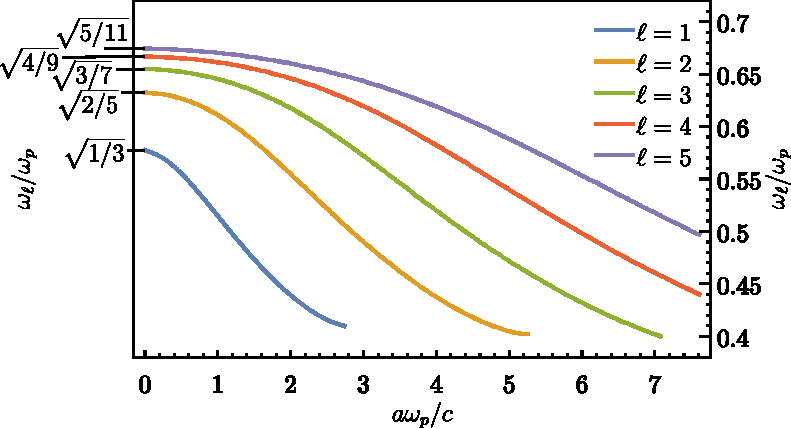
\includegraphics[scale=1]{1-Teoria/figs/1-4-DrudeMultipoles.pdf}\vspace*{-1em}
	\caption{Frecuencias de resonancia $\omega_\ell/\omega_p$ para una esfera con una función dieléctrica tipo Drude, como función del parámetro adimensional  $\omega_p a / c$, para los multipolos $\ell = 1,2,3$ y $4$. }
	\label{fig:NormalModes}
	\end{figure}			
	
Si se emplea la función dieléctrica del modelo de Drude-Sommerfeld [Ec.  \eqref{eq:Drude}] para $\omega = \omega_\ell$	y se sustituye en la Ec.  \eqref{eq:NormalModes}, al despejar $\omega_\ell$ tras considerar además el límite $\gamma\to 0$, la expresión para la frecuencia de resonancia del  modo normal del multipolo $\ell$ es \cite{maciel2017momentum}
	\begin{align}
	\frac{\omega_\ell}{\omega_p} = \sqrt{ \frac{\ell}{2\ell+1}}. \label{eq:PPequeña}
	\end{align}
Adicionalmente, si se considera la contribución de todos los órdenes multipolares ($\ell\to \infty$), la mayor frecuencia de resonancia es $\omega_\infty = \omega_p/\sqrt{2}$, que corresponde a la SPR de superfice.	
	
Para partículas esféricas de radio arbitrario $a$ con una función dieléctrica dada por el modelo de Drude-Sommerfeld, la frecuencia de resonancia $\omega_\ell$ sufre un corrimiento al rojo debido al tiempo de acomplamiento $a/c$ entre la interacción EM de la esfera y  la densidad de carga inducida que corresponde al plasmón de superficie \cite{aizpurua1998coupling}.  En la Fig.  \ref{fig:NormalModes} se muestran las frecuencias de resonancia $\omega_\ell$ normalizadas respecto a la frecuancia de plasma $\omega_p$, como función del parámetro adimensional $a\omega_p / c$ para los multipolos $\ell = 1,2,3$ y $4$.  El límite de partícula pequeña [Ec.  \eqref{eq:PPequeña}]	se recupera cuando  $a\to 0$ (lado izquierdo de la gráfica en la Fig.  \ref{fig:NormalModes}).  Para una función dieléctrica arbitraria, los modos normales se calculan como la frecuencia a la que la partícula extingue\footnote{Extinción se entiende como la pérdida de luz ocacionada por la absorción y esparcimiento de luz de la partícula; esta relación es conocida como el  \emph{teorema óptico} \cite{bohren1998absorption}. } la mayor cantidad de luz \cite{kreibig1995clusters}. 


\section{Modelo de esparcimiento coherente}


La solución de Mie, en conjunto con la corrección por tamaño de la función dieléctrica para algún material, permite estudiar la respuesta electromagnética (EM) de una nanopartícula (NP) esférica individual, tales como los plasmones localizados de superficies (Localized Surface Plasmons, LSPs), lo cuales son empleados en la espectroscopía \cite{novotny2006principles}, el sensado \cite{jain2008noble}, la litografía \cite{stockman2011nanoplasmonics}. Sin embargo, no siempre es posible emplear la respuesta EM de una partícula individual para la descripción del sistema por lo que se han empleado diversos enfoques entre los que se encuentran la aproximación cuasiestática y las teorías de esparcimiento \cite{pena-gomar2006coherent}. En el caso límite de partícula pequeña, donde el parámetro de tamaño $x=ka= 2\pi n_m$, con $n_m$  el índice de refracción del medio donde se encuentra inmersa NP, es mucho menor que la unidad, es posble emplear  la aproximación cuasiestática, que considera que sólo la excitación dipolar contribuye al campo total. En partícular, para la reflectancia de una monocapa de NPs, la aproximación cuasiestática conduce a una teoría de medio efectivo \cite{pena-gomar2006coherent}. Sin embargo, cuando  el parámetro de tamaño es comparable o mayor a la unidad, una teoría de esparcimiento es necesaria, debido a la inducción de multipolos de ordenes mayores \cite{pena-gomar2006coherent}. El modelo de esparcimiento coeherente (CSM) toma en cuenta la interacción de esparcidores puntuales ante la presencia de un campo eléctrico promedio; este acercamiento además incluye la contribución del esparcimiento múltiple debido a la interacción entre las NPs.
    
    El cálculo de las expresiones de reflectancia y transmitancia en el formalismo del CSM considera el campo eléctrico total esparcido por una monocapa de NPs. En general, éste puede descomponerse en una componente coherente ---respuesta promedio con una dirección de propagación bien definida--- y una componente difusa ---causada por las fluctuaciones y cuya propagación es en todas las direcciones--- \cite{tsang2000scattering}. Para definir los coeficientes de amplitud de reflexión y transmisión de la manera usual, se toma en cuenta  únicamente la componente coherente al asumir que la difusa es mucho menor que la coherente. Asimismo, primero se calculan los coeficientes de amplitud de reflexión y transmisión de una monocapa de NPs suspendida en el espacio libre (Free Standing Monolayer, FSM), es decir, inmersa en un medio dieléctrico denominado matriz, seguido del efecto de introducir una interfaz con un medio denominado sustrato. La reflectancia del sistema sustrato-matriz-monocapa se resuelve al considerar  multiples reflexiones en la interfaz entre las superficies dadas por la interfaz sutrato-matriz y matriz-monocapa. Este acercamiento evita el  cálculo de la contribución de partículas \emph{imagen} causadas por la  interfaz entre los dieléctricos y es consistente con la aproximación de campo efectivo ---en donde el campo eléctrico local es aproximado por el campo eléctrico promedio--- \cite{reyes2018analytical}.
 
\subsection{Monocapa suspendida en el espacio libre}
 
Para calcular los coeficientes de amplitud de reflexión y transmisión del CSM se calcula el campo eléctrico promedio esparcido por las NPs dentro de la región del espacio, caracterizado en su totalidad por el índice de refracción real $n_m$, delimitada por  $-d/2<z<d/2$, una placa de longitud $d$ y volumen $V$, en donde se encuentran $N$ NPs esféricas e idénticas y distribuidas espacialmente de forma aleatoria. Si una onda plana $\vb{E}^i = E_0 e^{i\vb{k}^i\cdot\vb{r}}\vu{e}_i$, donde se omite la dependecia temporal, y donde $\vu{e}_i$ es un vector en el plano de polarización de la onda plana y $|\vb{k}^i| = k = 2\pi n_m /\lambda$, incide sobre la placa, el campo eléctrico esparcido  por las NPs dentro de la placa $\vb{E}^s$, al suponer que la densidad $N/V$ es baja, puede calcularse bajo la aproximación de esparcidor individual (Single Scatterer Approximation, SSA), en donde cada NP esparce la luz sin considerar la interacción entre el campo eléctrico esparcido por las otras \cite{barrera2003coherent}. 

\begin{figure}[h!]\centering
	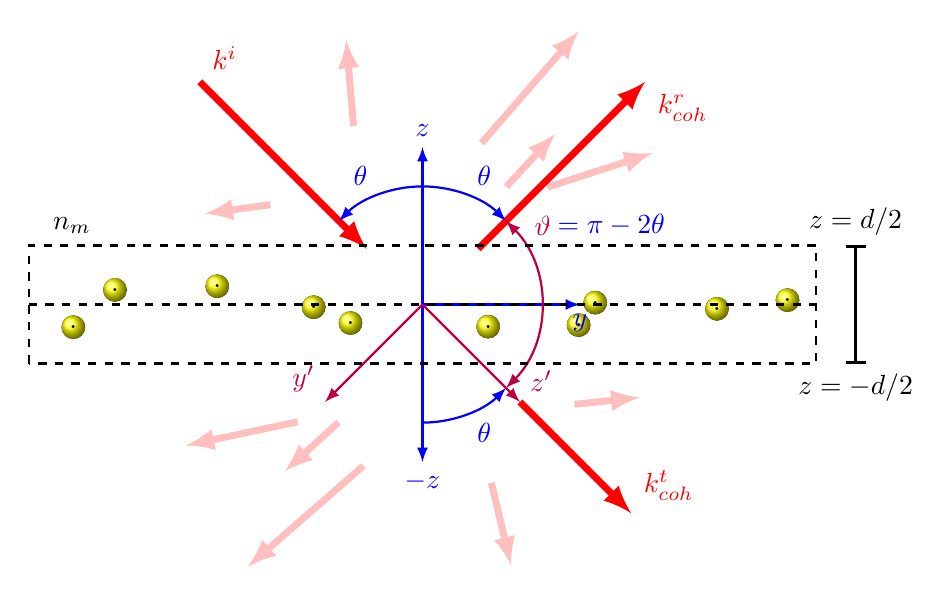
\begin{tikzpicture}[scale=1]
\def\a{.15}
\def\d{.75}
%----------------------NPs--------------
\foreach \y in {-4.5,-3.5,...,3.5,4.5}{
\fill[ball color=yellow, opacity=1] (\y+rand*.5,rand*.45) circle(\a) node[ ]{.};
}

%----------------------difussed scattered field--------------
\begin{scope}[opacity=.25, transparency group]
\foreach \s in {-1,1}{
	\draw[- latex, red, line width=2.5](0,\s*\d)++(25:\s*1.75)--(35+rand*5:\s*3.5);
	\draw[- latex, red, line width=2.5](0,\s*\d)++(35:\s*1.3)--(55+rand*5:\s*2.75);
	\draw[- latex, red, line width=2.5](0,\s*\d)++(165:\s*2)--(155+rand*5:\s*3);
	\draw[- latex, red, line width=2.5](0,\s*\d)++(120:\s*1.75)--(110+rand*5:\s*3.5);
	\draw[- latex, red, line width=2.5](0,\s*\d)++(60:\s*1.5)--(60+rand*5:\s*4);}
\end{scope}

%----------------------coherent scattered field--------------
\draw[latex -, thick, red, line width=2.5](135:1)--(135:4) node[anchor=south west]{$\vb{k}^i$};
\draw[- latex, thick, red, line width=2.5](45:1)--(45:4)node[anchor=north west]{$\vb{k}_{coh}^r$};
\draw[ - latex, thick, red, line width=2.5](-45:1.75)--(-45:3.75) node[anchor=south west]{$\vb{k}_{coh}^t$};

%----------------------Main system--------------
\draw[- latex, thick, blue] (0,0)--(90:2) node[anchor = south]{$z$};
\draw[- latex, thick, blue] (0,0)--(-90:2) node[anchor = north]{$-z$};
\draw[- latex, thick, blue] (0,0)--(0:2) node[anchor = north]{$y$};
\path (0,0)++(135/2:1.5)node[anchor=south west, blue]{$\theta$}; 
\draw[- latex, thick, blue](90:1.5)arc(90:45:1.5);
\path (0,0)++(-135/2:1.5)node[anchor=north west, blue]{$\theta$}; 
\draw[- latex, thick, blue](-90:1.5)arc(-90:-45:1.5);
\path (0,0)++(90+45/2:1.5)node[anchor=south east, blue]{$\theta$}; 
\draw[- latex, thick, blue](90:1.5)arc(90:135:1.5);

----------------------Mie system--------------
\draw[- latex, thick, purple] (0,0)--(-45:1.75) node[anchor = south west]{$z'$};
\draw[- latex, thick, purple] (0,0)--(-135:1.75) node[anchor = south east]{$y'$};
\path (0,0)++(30:1.5)node[anchor=south west, purple]{$\vartheta$}; 
\path (0,0)++(30:1.5)node[anchor=south west, blue]{$\;\;\; =  \pi - 2\theta$}; 
\draw[latex - latex, thick, purple](-45:1.5)arc(-45:45:1.5);

%----------------------thickness and slab-------------
\draw[thick, dashed] (-5,-\d) rectangle (5,\d);
\draw[thick, dashed] (-5, 0) --  (5,0);
\draw[ |-|, thick,] (5.5,-\d) node[anchor = north]{$z=-d/2$} -- (5.5,\d) node[anchor = south]{$z=d/2$};
\node at (-4.5,1) {$\; n_m$};
\end{tikzpicture}
	\caption{  Película de grosor $d$ con y volumen $V$ con $N$ partículas esféricas idénticas y una onda incidente en la dirección $\vb{k}^i$. La dirección de los campos esparcidos coeherentes están dadas por $\vb{k}^r_{coh}$ y $\vb{k}^t_{coh}$. Las flechas rojas sólidas representan las componentes coehrentes del campo esparcido mientras que las rosas represetan su componente difusa. }\label{fig:CSM-Slab}
	\end{figure}


Al considerar la interacción del campo eléctrico incidente con las $N$ NPs dentro de la placa, el campo eléctrico esparcido por todas las partículas tiene componentes espaciales en todas las direcciones, por lo que le campo eléctrico esparcido puede descomponerse en una componente coherente y una difusa. El  campo eléctrico esparcido promedio $\langle \vb{E}^s\rangle$, que corresponde a la componente coherente, se calcula al considerar el promedio espacial de las NPs dentro de la placa al suponer que la posición de una NPs es independiente de la de las demás y que la probabilidad de encontrar el centro de una NPs, punto negro dentro de las NPs en la Fig. \ref{fig:CSM-Slab},  dentro del volumen de la placa es uniforme, por lo que la componente coherente del campo esparcido es  \cite{garcia2012multiple} 
	\begin{align}
	\langle \vb{E}^s\rangle =
	\begin{dcases} 
	      \langle \vb{E}^s_{r,SSA}\rangle e^{i\vb{k}^r_{coh}\cdot\vb{r}} =
	    			i \frac{N}{V}  \frac{d E_0}{2} \frac{\sin(k_z^id)}{k_z^i d} 
				\frac{\mathbb{F}(\vu{k}^r,\vu{k}^i)\cdot \vu{e}_i}{k_z^i }	e^{i\vb{k}^r_{coh}\cdot\vb{r}},									& d/2<z \\
      \langle \vb{E}^s_{t,SSA}\rangle e^{i\vb{k}^t_{coh}\cdot\vb{r}} =
 				i\frac{N}{V} \frac{d E_0}{2}\frac{\mathbb{F}(\vu{k}^i,\vu{k}^i)\cdot \vu{e}_i}{k_z^i}		
				e^{i\vb{k}^t_{coh}\cdot\vb{r}},
							& z<-d/2
   \end{dcases}
   	\label{eq:AvErEt}
	\end{align}
en donde $k^i_z = k^i\cos\theta$; $\vb{k}^i$ es el vector de onda del campo eléctrico incidente $\vb{E}^i = \vb{E}_0 e^{i\vb{k}^i\cdot\vb{r}}$, polarizado en la dirección $\vu{e}_i$; $\vb{k}^r_{coh}$ es la dirección de propagación de la componente coherente reflejada; $\vb{k}^t_{coh}=\vb{k}^i$, de la componente coherente transmitida; y $\mathbb{F}$ es la diadica de esparcimiento de campo lejano [Ec. \eqref{eq:FarFieldDyadic}] que depende de la dirección de propagación de la onda plana incidente $\vb{k}^i$ y la del campo esparcido $\vb{k}^s$; el término de $\mathbb{F}$ no limita la solución del campo eléctrico esparcido promedio al campo lejano puesto que es un resultado derivado del promediar la respuesta EM \cite{gutierrez2012overview}. En la Fig, \ref{fig:CSM-Slab} se observa que la dirección de propagación de  $\langle \vb{E}^s_{r,SSA}\rangle$ en $d/2<z$ y la de $\langle \vb{E}^s_{t,SSA}\rangle$ en  $z<-d/2$ es de $\theta$ respecto a la dirección normal a la monocapa (sitema coordenado azul). Asimismo, se muestra en rojo claro la componente difusa del campo eléctrico esparcido que, al calcular el campo esparcido promedio, es nula. A diferencia la componente difusa, la componente coherente del campo eléctrico esparcido es distinta de cero ya que los campos eléctricos esparcidos por cada NP en la placa interfieren constructivamente en las direcciones de esparcimiento $\vu{k}^s =\vu{k}^i=\vu{k}^t_{coh}$ y $\vu{k}^s =\vu{k}^r_{coh}$ \cite{garcia2012multiple}. Puesto que las NPs dentro de la placa son esféricas e idénticas, se calcula la expresión de la diadica de esparcimiento $\mathbb{F}(\vu{k}^s,\vu{k}^i)$ al comparar su expresión general [Ec. \eqref{eq:FarFieldDyadic}] con la matriz de esparcimiento de Mie [Ec. \eqref{eq:MieMatrix}], por lo que la diadica de esparcimiento de campo lejano es
	\begin{align}
	\mathbb{F}(\vu{k}^s,\vu{k}^i) = \frac{1}{-ik} 
	 \mqty(S_2(\vartheta) & 0 \\ 0 & S_1(\vartheta)),
	 \label{eq:FFDydadic-Mie}
	\end{align}
en donde ángulo entre la dirección del campo esparcido $\vu{k}^s$ y del campo incidente $\vu{k}^i$, se denota con $\vartheta$ que toma los valores $\vartheta = 0$ para $\vu{k}^s = \vu{k}^t_{coh}$ y $\vartheta = \pi-2\theta$  para $\vu{k}^s = \vu{k}^r_{coh}$ como se observa en la Fig. \ref{fig:CSM-Slab}.
	
Al sustituir la Ec. \eqref{eq:FFDydadic-Mie} en la Ec. \eqref{eq:AvErEt} y multiplicar las expresiones resultantes por $(3ka^3)/(3ka^3)$, con $a$ el radio de las NPs y $k = 2\pi n_m /\lambda$, y agrupar términos, se llegan a las expresiones 
	\begin{subequations}\begin{align}
		\langle \vb{E}^s_{r,SSA}\rangle & = - \frac{E_0}{\cos\theta_i} \frac32  \qty(\frac{N}{V} \frac43\pi a^3)\frac{kd}{(ka)^3}   \frac{\sin(k_z^id)}{k_z^i d}  S_n(\vartheta)\vu{e}_i =
		-\alpha  \frac{\sin(k_z^id)}{k_z^i d}   S_n(\vartheta) \vb{E}_0,
		\label{eqs:EsSSAr}\\
	\langle \vb{E}^s_{t,SSA}\rangle &=  - \frac{E_0}{\cos\theta_i} \frac32
						 \qty(\frac{N}{V}\frac43\pi a^3  ) \frac{kd}{(ka)^3}  S_n(0) \vu{e}_i  
						 = - \alpha S(0) \vb{E}_0
		\label{eqs:EsSSAt}
	\end{align}\label{eq:EsSSA}\end{subequations}
donde  se emplea $n=1$ para polarización $s$ y $n_2$ para $p$ en las entradas no nulas de la matriz de esparcimiento de Mie $S_n(\vartheta)$ y donde se define $S(0) \equiv S_1(0)=S_2(0)$. Al sustituir con el parámetro de tamaño $x=ka$ se obtiene que  
\begin{align*}
	\alpha \equiv \frac32 \qty(\frac{N}{V}\frac43 \pi a^3  )\frac{kd}{x^3\cos\theta_i)} = \frac32\frac{kd}{ x^3\cos\theta_i} f,
	\end{align*}
con $f= N 4\pi a^3/(3V)$ la fracción de llenado que es el cociente entre el neto de las NPs entre el volumen de la placa. Si se considera el límite $d\to 0$, lo que equivale a tener una monocapa de partículas esféricas desordenadas y al asumir que la componente difusa del campo esparcido por las partículas es despreciable en comparación a la componente coherente, es posible definir los coeficientes de amplitud de reflexión y transimisión en la SSA a partir de las Ecs. \eqref{eq:EsSSA} como \vspace*{-.5em}	
	
	\begin{subequations}\eqhalf{r_{coh}^{SSA} = -\alpha S_n(\vartheta),}
	\eqhalf{t_{coh}^{SSA} = 1 - \alpha S(0), }
	\label{eq:rtcohSSA}\end{subequations}\vspace*{-.5em}	
	
\noindent en donde para el coeficiente de amplitud de transmisión se suma la contribución de la onda plana a la Ec. \eqref{eqs:EsSSAt}, y al considerar que $V = A d$, el coeficiente $\alpha$ se reescribe como
	\begin{align}
	\alpha = \frac{2\Theta}{x^2 \cos\theta_i}
	\label{eq:alpha}
	\end{align}
donde $\Theta = N \pi a^2 / A$ es la fracción de cubierta que corresponde al área proyectada por las esferas sobre el área de la placa. Al analizar  las Ecs. \eqref{eq:rtcohSSA} y \eqref{eq:alpha}, para ángulos rasantes $\theta\to \pi/2$ se observa que $\alpha\to \infty$, además de que para partículas pequeñas $x\ll 1$ el producto $r_{coh}^{SSA}r_{coh}^{SSA*}$ puede tomar valores mayores a la unidad. Por tanto los coeficientes de amplitud calculadas a partir de la SSA son válidos únicamente para ángulos de incidencia no rasantes y para partículas grandes. 

Para calcular coeficientes de amplitud a partir de la SSA pero que no estén límitados a ángulos de incidencia bajos ni al tamaño de las partículas que conforman a la monocapa, se deben considerar contribuciones de esparcimiento múltiple (Multiple Scattering, MS) en el cálculo del campo eléctrico $\vb{E}^{exc}$  que excita a las partículas dentro de la placa, el cual se puede descomponer como 
	\begin{align}
	\vb{E}^{exc} = \vb{E}^{exc}_{t} e^{i\vb{k}^t_{coh}\cdot\vb{r}}+
					\vb{E}^{exc}_{r} e^{i\vb{k}^r_{coh}\cdot\vb{r}}
	\end{align}
donde  $\vb{E}^{exc}_t$ tiene la misma polarización y dirección de propagación de $\langle \vb{E}^s_{t,SSA}\rangle$  y $\vb{E}^{exc}_{r}$, de $\langle \vb{E}^s_{r,SSA}\rangle$, de las Ecs. \eqref{eq:EsSSA}, como se observa en la Fig. \ref{fig:MScatt-slab-MS}. Entonces, el campo eléctrico esparcido promedio considerando el MS $\vb{E}^s_{MS}$, toma en cuenta  las reflexiones y transmisiones de $\vb{E}^{exc}$ según las Ecs. \eqref{eq:EsSSA} en el límite $d\to 0$ \cite{gutierrez2012overview}, y la contribución del campo eléctrico incidente $\vb{E}^i$, por lo que  \cite{reyes2018analytical}
	\begin{subequations}\begin{align}
		\langle \vb{E}^s_{r,coh}\rangle & =	\langle \vb{E}^s_{r,MS}\rangle
					= \qty[-\alpha S_n(\vartheta)E^{exc}_t -\alpha S(0)E^{exc}_r
					]\vu{e}_i e^{i\vb{k}^r_{coh}\cdot\vb{r}},\\
		\langle \vb{E}^s_{t,coh}\rangle & =\vb{E}^i+\langle\vb{E}^s_{r,MS}\rangle
					= \qty[E_0 -\alpha S(0)E^{exc}_t 
					-\alpha	 S_n(\vartheta)E^{exc}_r
					]\vu{e}_i e^{i\vb{k}^t_{coh}\cdot\vb{r}}.
	\end{align} \label{eq:EsMS}\end{subequations}

	\begin{figure}[h!]\centering
		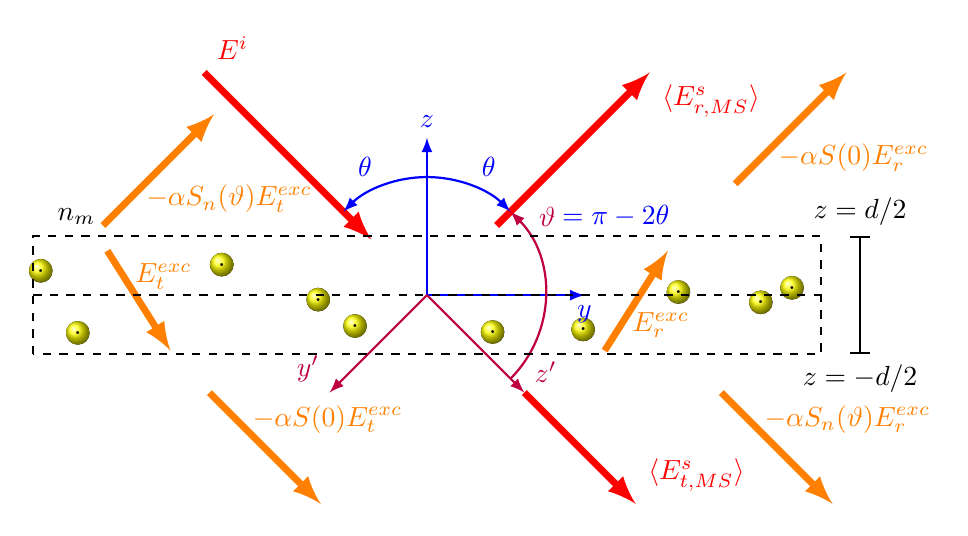
\begin{tikzpicture}[scale=1]
\def\a{.15}
\def\d{.75}

%----------------------NPs--------------
\foreach \y in {-4.5,-4.5,-2.5,-1.5,-.5,.5,1.5,3.5,4,4.5}{
\fill[ball color=yellow, opacity=1] (\y+rand*.5,rand*\d) circle(\a) node[ ]{.};
}

%----------------------averged fields ---------------------
\draw[latex -, thick, red, line width=2.5](135:1)--(135:4) node[anchor=south west]{$\vb{E}^i$};
\draw[- latex, thick, red, line width=2.5](45:\d+.5)--(45:4)node[anchor=north west]{$\langle\vb{E}_{r,MS}^s\rangle$};
\draw[ - latex, thick, red, line width=2.5](-45:1.75)--(-45:3.75) node[anchor=south west]{$\langle\vb{E}_{t,MS}^s\rangle$};

%---------------------- Exciting fields ---------------------
\draw[- latex , thick,  orange, line width=2.5,shift ={(-3,0)}](152:1.2)node[anchor= north west]{$\;\;\vb{E}^{exc}_t$}--(250:\d);
\draw[latex - , thick, orange, line width=2.5,shift ={(2,0)}](28:1.2)--(-70:\d) node[anchor= south west]{$\;\;\vb{E}^{exc}_r$};

%-------------- reflected and transmitted exciting fields UP ---------------------
\draw[latex - , thick, orange, line width=2.5,shift={(2.5, 0)}](-45:3.75)--(-45:1.75) node[anchor=north west]{$\;\;\;\;-\alpha S_n(\vartheta)\vb{E}^{exc}_r$};
\draw[latex - , thick, orange, line width=2.5,shift={(-4, 0)}](-45:3.75)--(-45:1.75) node[anchor=north west]{$\;\;\;\;-\alpha S(0)\vb{E}^{exc}_t$};

%-------------reflected and transmitted exciting fields DOWN ---------------------
\draw[latex -, thick, orange, line width=2.5,shift={(2.5, 0)}](45:4)--(45:2)node[anchor=south west]{$\;\;\;\;-\alpha S(0) \vb{E}^{exc}_r$};
\draw[latex -, thick, orange, line width=2.5,shift={(-5, 0)}](45:3.25)--(45:\d+.5)node[anchor=south west]{$\;\;\;\;-\alpha S_n(\vartheta) \vb{E}^{exc}_t$};

%----------------------main system---------------------
\draw[- latex, thick, blue] (0,0)--(90:2) node[anchor = south]{$z$};
\draw[- latex, thick, blue] (0,0)--(0:2) node[anchor = north]{$y$};
\path (0,0)++(135/2:1.5)node[anchor=south west, blue]{$\theta$}; 
\draw[- latex, thick, blue](90:1.5)arc(90:45:1.5);
\path (0,0)++(90+45/2:1.5)node[anchor=south east, blue]{$\theta$}; 
\draw[- latex, thick, blue](90:1.5)arc(90:135:1.5);

%----------------------Mie system---------------------
\draw[- latex, thick, purple] (0,0)--(-45:1.75) node[anchor = south west]{$z'$};
\draw[- latex, thick, purple] (0,0)--(-135:1.75) node[anchor = south east]{$y'$};
\path (0,0)++(30:1.5)node[anchor=south west, purple]{$\vartheta$}; 
\path (0,0)++(30:1.5)node[anchor=south west, blue]{$\;\;\; =  \pi - 2\theta$}; 
\draw[- latex, thick, purple](-45:1.5)arc(-45:45:1.5);

%----------------------thickness and slab ---------------------
\draw[thick, dashed] (-5,-\d) rectangle (5,\d);
\draw[thick, dashed] (-5, 0) --  (5,0);
\draw[ |-|, thick,] (5.5,-\d) node[anchor = north]{$z=-d/2$} -- (5.5,\d) node[anchor = south]{$z=d/2$};
\node at (-4.5,1) {$\; n_m$};
\end{tikzpicture}
		\caption{  Película de grosor $d\to 0$ con y volumen $V$ con $N$ partículas esféricas idénticas y una onda incidente en la dirección $\vb{k}^i$. La dirección de los campos esparcidos coeherentes están dadas por $\vb{k}^r_{coh}$ y $\vb{k}^t_{coh}$. Las flechas rojas sólidas representan las componentes coehrentes del campo esparcido mientras que las rosas represetan su component difusa. }\label{fig:MScatt-slab-MS}
	\end{figure}	
	
	
Para determinar la expresión del campo eléctrico que excita a las NPs en la placa $\vb{E}^{exc}$ considerando el MS\footnote{El procedimiento descrito en este texto emplea un enfoque heurístico que se publicó en \cite{reyes2018analytical} sin emabargo, un enfoque más riguroso se encuentra en \cite{barrera2003coherent}.}, se divide la placa donde se encuentras las NPs en dos de grosor $d/2$, y se calcula el promedio de  $\vb{E}^{exc}$ en la interfaz entre las dos placas ($z=0$) mediante autoconsistencia, por lo que las NPs en la placa no sólo son iluminadas por el campo eléctrico incidente $\vb{E}^i$, sino también por $\vb{E}^{exc}$ \cite{reyes2018analytical}. La componente de $\vb{E}^{exc}$ que se propaga en la dirección del campo eléctrico incidente $\vb{E}^{exc}_{t}$ se calcula como el campo incidente más los campos esparcidos por las NPs es la placa superior ($0<z<d/2$) que son  igual a la suma del la transmisión del campo $E^{exc}_t$ y a la reflexión del campo $E^{exc}_r$ por la placa superior, es decir,
	\begin{subequations}\begin{align}
		\vb{E}^{exc}_t  e^{i\vb{k}^i\cdot\vb{r}}  =
				\qty[E_0  - \frac12 \qty(
					\alpha S(0)E^{exc}_t + \alpha S_n(\vartheta)E^{exc}_r
				)] e^{i\vb{k}^t_{coh}\cdot\vb{r}}  \vu{e}_i.
	\end{align}
donde el factor de $1/2$ considera que es la respuesta promedio dentro de la placa. Asimismo, el campo $\vb{E}^{exc}_{r}$ se calcula como la reflexión  del campo $E^{exc}_t$ y a la transmisión del campo $E^{exc}_r$ por la placa inferior ($-d/2<z<0$), por lo que su expresión es	
	\begin{align}
	\vb{E}^{exc}_r  e^{i\vb{k}^r\cdot\vb{r}}  =
				\qty[- \frac12 \qty(
					\alpha S_n(\vartheta)E^{exc}_t + \alpha S(0)E^{exc}_r
				)] e^{i\vb{k}^r_{coh}\cdot\vb{r}}  \vu{e}_i.
	\end{align} \label{eq:Eexc}\end{subequations}
En la Fig. \ref{fig:Eexc} se muestra una representación gráfica de las Ecs. \eqref{eq:Eexc}, que són válidas únicamente en $-d/2<z<d/2$.

\begin{figure}[h!]\centering
	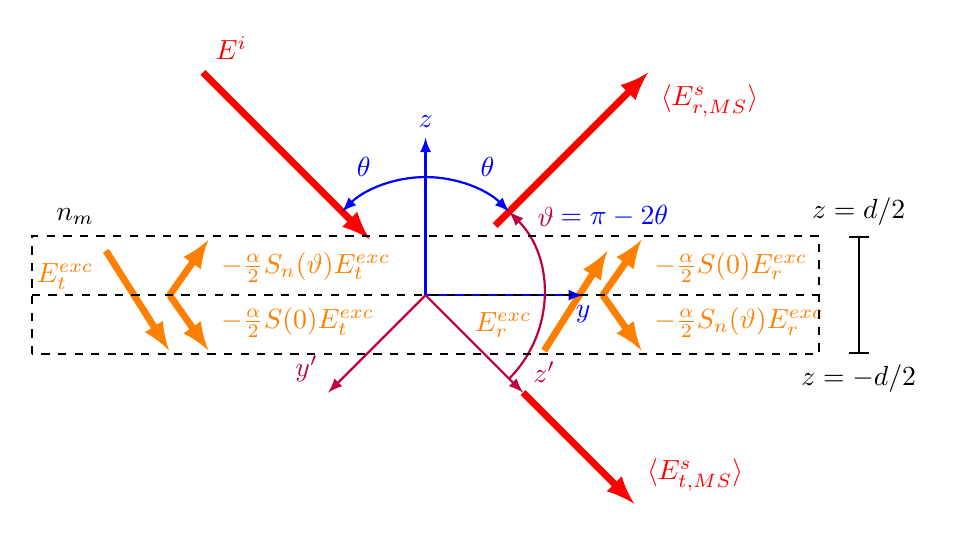
\begin{tikzpicture}[scale=1]
\def\a{.15}
\def\d{.75}

%\foreach \y in {-4.5,-3.5,-2.5,-.5,.5,2.5,3.5,4.5}{
%\fill[ball color=yellow, opacity=1] (\y+rand*.5,rand*\d) circle(\a) node[ ]{.};
%}


\draw[latex -, thick, red, line width=2.5](135:1)--(135:4) node[anchor=south west]{$\vb{E}^i$};
\draw[- latex, thick, red, line width=2.5](45:\d+.5)--(45:4)node[anchor=north west]{$\langle\vb{E}_{r,MS}^s\rangle$};
\draw[ - latex, thick, red, line width=2.5](-45:1.75)--(-45:3.75) node[anchor=south west]{$\langle\vb{E}_{t,MS}^s\rangle$};

%---------------------- Exciting transmitted field ---------------------
\draw[latex - , thick,  orange, line width=2.5,shift={(-3., 0)}](250:\d)--(152:1.2) node[anchor= north east]{$\vb{E}^{exc}_t$};

\draw[- latex , thick,  orange, line width=2.5, shift={(-2.5, 0)}](180:\d)--(250:\d) node[anchor= south west]{$-\frac{\alpha}{2} S(0)\vb{E}^{exc}_t$};
\draw[- latex , thick,  orange, line width=2.5, shift={(-2.5, 0)}](180:\d)--(110:\d) node[anchor= north west]{$-\frac{\alpha}{2} S_n(\vartheta)\vb{E}^{exc}_t$};

%---------------------- Exciting reflected field ---------------------
\draw[ latex -, thick, orange, line width=2.5,shift={(1.25, 0)}](28:1.2)--(-70:\d) node[anchor= south east]{$\vb{E}^{exc}_r$};

\draw[- latex , thick,  orange, line width=2.5, shift={(3., 0)}](180:\d)--(250:\d) node[anchor= south west]{$-\frac{\alpha}{2} S_n(\vartheta)\vb{E}^{exc}_r$};
\draw[- latex , thick,  orange, line width=2.5, shift={(3., 0)}](180:\d)--(110:\d) node[anchor= north west]{$-\frac{\alpha}{2}S(0)\vb{E}^{exc}_r$};

%----------------------Main system---------------------
\draw[- latex, thick, blue] (0,0)--(90:2) node[anchor = south]{$z$};
\draw[- latex, thick, blue] (0,0)--(0:2) node[anchor = north]{$y$};
\path (0,0)++(135/2:1.5)node[anchor=south west, blue]{$\theta$}; 
\draw[- latex, thick, blue](90:1.5)arc(90:45:1.5);
\path (0,0)++(90+45/2:1.5)node[anchor=south east, blue]{$\theta$}; 
\draw[- latex, thick, blue](90:1.5)arc(90:135:1.5);

%----------------------Mie system---------------------
\draw[- latex, thick, purple] (0,0)--(-45:1.75) node[anchor =south west]{$z'$};
\draw[- latex, thick, purple] (0,0)--(-135:1.75) node[anchor =south east]{$y'$};
\path (0,0)++(30:1.5)node[anchor=south west, purple]{$\vartheta$}; 
\path (0,0)++(30:1.5)node[anchor=south west, blue]{$\;\;\; =  \pi - 2\theta$}; 
\draw[- latex, thick, purple](-45:1.5)arc(-45:45:1.5);

%----------------------thickness and slab ---------------------
\draw[thick, dashed] (-5,-\d) rectangle (5,\d);
\draw[thick, dashed] (-5, 0) --  (5,0);
\draw[ |-|, thick,] (5.5,-\d) node[anchor = north]{$z=-d/2$} -- (5.5,\d) node[anchor = south]{$z=d/2$};
\node at (-4.5,1) {$\; n_m$};

\end{tikzpicture}
	\caption{  Película de grosor $d\to 0$ con y volumen $V$ con $N$ partículas esféricas idénticas y una onda incidente en la dirección $\vb{k}^i$. La dirección de los campos esparcidos coeherentes están dadas por $\vb{k}^r_{coh}$ y $\vb{k}^t_{coh}$. Las flechas rojas sólidas representan las componentes coehrentes del campo esparcido mientras que las rosas represetan su componente difusa. }\label{fig:Eexc}
	\end{figure}	
	

Al resolver para $E^{exc}_t$ y $E^{exc}_r$ se obtienen las expresiones
	\begin{align}
	\vb{E}^{exc}_t  &= \frac{\qty[1+\frac12\alpha S(0)]}
				{1+\alpha S(0) +\frac14\alpha^2\qty[S^2(0)-S_n^2(\vartheta)]}\vb{E}_0,\\
	\vb{E}^{exc}_r  &= \frac{-\frac12\alpha S_n(\vartheta)}
				{1+\alpha S(0) +\frac14\alpha^2\qty[S^2(0)-S_n^2(\vartheta)]}\vb{E}_0.
	\end{align}
por lo que, al sustituilas en las expresiones de los campos esparcidos promedio reflejados y transmitidos [Ecs. \eqref{eq:EsMS}] se obtienen
	\begin{align*}
	\langle \vb{E}^s_{r,coh}\rangle &=
			\frac{-\alpha S_n(\vartheta)}{1+\alpha S(0)+\frac14 \alpha^2 \left[S^2(0)-S_n^2 (\vartheta) \right]} \vb{E}_0 e^{i\vb{k}^r_{coh}\cdot\vb{r}},\\
	\langle \vb{E}^s_{r,coh}\rangle &=
			\frac{1-\frac14\alpha^2\qty[S^2(0)-S_n^2(\vartheta)]}{1+\alpha S(0)+\frac14 \alpha^2 \left[S^2(0)-S_n^2 (\vartheta) \right]} \vb{E}_0 e^{i\vb{k}^t_{coh}\cdot\vb{r}},
	\end{align*}
de donde es posible calcular los coeficientes de amplitud del CSM al considerar que $\vartheta = \pi-2\theta$, que el campo eléctrico que excita a las NPs toma en cuenta el esparcimiento múltiple y que la componente coherente del campo esparcido es mucho mayor que la contribución de la componente difusa, dando como resultado \vspace*{-.5em}
	\begin{subequations}\begin{tcolorbox}[title = Coeficientes de amplitud del CSM, ams align, breakable ]
	r_{coh}&=\frac{-\alpha S_n(\pi-2\theta)}
				{1+\alpha S(0)+\frac14 \alpha^2 \left[S^2(0)-S_n^2 (\pi-2\theta) \right]},
			\label{eqs:rcoh}\\
	t_{coh}&=\frac{1-\frac14\alpha^2\qty[S^2(0)-S_n^2(\pi-2\theta)]}
				{1+\alpha S(0)+\frac14 \alpha^2 \left[S^2(0)-S_n^2 (\pi-2\theta) \right]}.
		\label{eqs:tcoh}
	\end{tcolorbox}\label{eq:rtcoh}\end{subequations}\vspace*{-.5em}\noindent


	 \subsection{Monocapa sobre un sustrato}
	 	Desarrollo de las multiples reflexiones dentro del sistema
